\documentclass[11pt,a4paper]{amsbook}
\usepackage[left=3cm,right=3cm,top=3cm,bottom=3cm]{geometry}
\usepackage[onehalfspacing]{setspace}
\usepackage[spanish]{babel}

\usepackage{amsmath, amssymb, amsthm}

\usepackage{hyperref}
\urlstyle{same}

\usepackage{tikz,tikz-cd}

\usepackage{bm}

\usepackage{adjustbox}
\usepackage{pdfpages}
\usepackage{graphicx}
\usepackage{epigraph}

\usepackage[scr=boondox]{mathalfa}

%\usepackage[backend=biber]{biblatex}
%\addbibresource{biblio_guillermo.bib}

\DeclareEmphSequence{\bfseries\itshape}

\newtheorem{thm}[subsection]{Teorema}
\newtheorem{prop}[subsection]{Proposición}
\newtheorem{conj}[subsection]{Conjetura}
\newtheorem{lemma}[subsection]{Lema}
\newtheorem{corol}[subsection]{Corolario}
\theoremstyle{remark} \newtheorem{rmk}[subsection]{Observación}
\theoremstyle{definition} \newtheorem{defn}[subsection]{Definición}
\theoremstyle{definition} \newtheorem{ex}[subsection]{Ejemplo}
\theoremstyle{definition} \newtheorem{ej}[subsection]{Ejercicio}

\makeatletter
\hypersetup{
	colorlinks,
	linkcolor=[rgb]{0.2,0.2,0.6},
	citecolor=[rgb]{0.2,0.6,0.2},
	urlcolor=[rgb]{0.6,0.2,0.2}}
\makeatother

\makeatletter
\@removefromreset{section}{chapter}
\makeatother


\renewcommand{\thechapter}{\Roman{chapter}}
\renewcommand{\thesection}{\arabic{section}}

\setcounter{tocdepth}{1}

\newcommand*{\todo}[1]{\textcolor{red}{(TO DO: #1)}}

% Math Bold
\newcommand{\C}{\mathbb C}
\newcommand{\RP}{\mathbb{RP}}
\newcommand{\CP}{\mathbb{CP}}
\newcommand{\Q}{\mathbb Q}
\newcommand{\Z}{\mathbb Z}
\newcommand{\N}{\mathbb N}
\newcommand{\RR}{\mathbb R}
\newcommand{\bbA}{\mathbb A}
\newcommand{\bbT}{\mathbb T}
\newcommand{\bbR}{\mathbb R}
\newcommand{\bbK}{\mathbb K}
\newcommand{\bbS}{\mathbb S}
\newcommand{\bbH}{\mathbb H}
\newcommand{\bbB}{\mathbb B}
\newcommand{\bbX}{\mathbb X}
\newcommand{\bbE}{\mathbb E}
\newcommand{\bbP}{\mathbb P}
\newcommand{\bbI}{\mathbb I}

% Calligraphic
\newcommand{\cA}{\mathcal A}
\newcommand{\cB}{\mathcal B}
\newcommand{\cC}{\mathcal C}
\newcommand{\cD}{\mathcal D}
\newcommand{\cE}{\mathcal E}
\newcommand{\cF}{\mathcal F}
\newcommand{\cH}{\mathcal H}
\newcommand{\ch}{\mathcal h}
\newcommand{\cG}{\mathcal G}
\newcommand{\cI}{\mathcal I}
\newcommand{\cJ}{\mathcal J}
\newcommand{\cK}{\mathcal K}
\newcommand{\cL}{\mathcal L}
\newcommand{\cM}{\mathcal M}
\newcommand{\cN}{\mathcal N}
\newcommand{\cO}{\mathcal O}
\newcommand{\cP}{\mathcal P}
\newcommand{\cR}{\mathcal R}
\newcommand{\cS}{\mathcal S}
\newcommand{\cT}{\mathcal T}
\newcommand{\cU}{\mathcal U}
\newcommand{\cV}{\mathcal V}
\newcommand{\cW}{\mathcal W}
\newcommand{\cX}{\mathcal X}
\newcommand{\cY}{\mathcal Y}
\newcommand{\cZ}{\mathcal Z}

% Fraktur
\newcommand{\fA}{\mathfrak A}
\newcommand{\fB}{\mathfrak B}
\newcommand{\fC}{\mathfrak C}
\newcommand{\fD}{\mathfrak D}
\newcommand{\fH}{\mathfrak H}
\newcommand{\fP}{\mathfrak P}
\newcommand{\fS}{\mathfrak S}
\newcommand{\fT}{\mathfrak T}
\newcommand{\fU}{\mathfrak U}
\newcommand{\fV}{\mathfrak V}
\newcommand{\fX}{\mathfrak X}
\newcommand{\fR}{\mathfrak R}
\newcommand{\fY}{\mathfrak Y}
\newcommand{\fZ}{\mathfrak Z}
\newcommand{\fL}{\mathfrak L}
\newcommand{\ff}{\mathfrak f}
\newcommand{\fm}{\mathfrak m}
\newcommand{\fn}{\mathfrak n}
\newcommand{\fs}{\mathfrak s}
\newcommand{\ft}{\mathfrak t}
\newcommand{\fg}{\mathfrak{g}}
\newcommand{\fz}{\mathfrak{z}}
\newcommand{\fE}{\mathfrak E}
\newcommand{\fh}{\mathfrak h}
\newcommand{\fa}{\mathfrak a}
\newcommand{\fc}{\mathfrak c}

% Script
\newcommand{\sC}{\mathscr C}
\newcommand{\sX}{\mathscr X}
\newcommand{\sD}{\mathscr D}
\newcommand{\sU}{\mathscr U}
\newcommand{\sO}{\mathscr O}
\newcommand{\sH}{\mathscr H}
\newcommand{\sF}{\mathscr F}
\newcommand{\sL}{\mathscr L}
\newcommand{\sG}{\mathscr G}
\newcommand{\sJ}{\mathscr J}
\newcommand{\sS}{\mathscr S}

% Sans Serif
\newcommand{\sfA}{\mathsf A}
\newcommand{\sfB}{\mathsf B}
\newcommand{\sfC}{\mathsf C}
\newcommand{\sfD}{\mathsf D}
\newcommand{\sfE}{\mathsf E}
\newcommand{\sfF}{\mathsf F}
\newcommand{\sfG}{\mathsf G}

% Miscellaneous
\DeclareMathOperator{\pr}{pr}
\DeclareMathOperator{\GL}{GL}

\title{Lecciones de Geometría Diferencial}
\author{Guillermo Gallego}

\begin{document}

\includepdf[pages=1]{portada.pdf}

\thispagestyle{empty}
\vfill
\footnote{Imagen de portada: \textit{El geógrafo y el naturalista}, por Adriaen van Stalbent}
\hrule

\frontmatter
\begin{titlepage}
\setcounter{page}{1}
\thispagestyle{empty}
\begin{center}
{\Large \bfseries LECCIONES DE GEOMETRÍA DIFERENCIAL} \par\vspace{2em}
{\large \textsc{Guillermo Gallego}} \par\bigskip
\end{center}

\vfill

\begin{center}
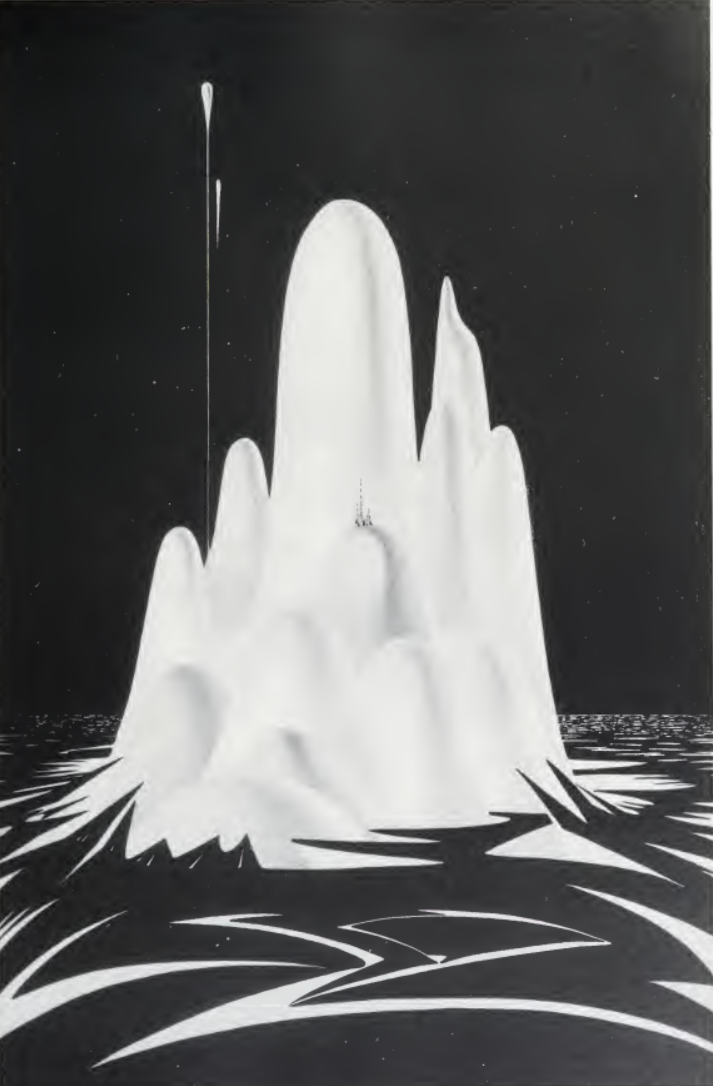
\includegraphics[width=0.7\textwidth]{fomenko.png} \\
\textit{Funciones de Morse y el teorema sobre la característica de Euler}, por A. Fomenko
\end{center}

\vfill
\hrule \vspace{1em}
\begin{center}
\textsc{Departamento de Matemáticas, Universidad Autónoma de Madrid} \\ \vspace{1em}
\textit{Email:} \normalfont\href{mailto:guillermo.gallego@uam.es}{guillermo.gallego@uam.es} \hspace{1em}
\textit{URL:} \normalfont\href{https://guillegallego.xyz}{https://guillegallego.xyz}
\end{center}
\end{titlepage}

\thispagestyle{empty}

\vspace*{\fill}

\newpage
\null
\thispagestyle{empty}

\epigraph{%
  Los encantos de esta ciencia sublime tan sólo se revelan en toda su belleza a aquellos con el valor para profundizar en ella.
}{Gauss}

\vspace*{\fill}

\newpage
\null
\thispagestyle{empty}
\newpage

{\tiny \tableofcontents}

\mainmatter

\chapter{Fundamentos de variedades diferenciables}


\section{Variedades diferenciables: definición y ejemplos}

\begin{defn}
  Un \emph{sistema de coordenadas de dimensión $n$} en un espacio topológico $M$ es un par $(U,\bm{x})$ formado por un abierto $U\subset M$ y un homeomorfismo $\bm{x}: U \rightarrow \bm{x}(U)\subset \RR^n$, con $\bm{x}(U)\subset \RR^n$ un subconjunto abierto.

  Una \emph{variedad topológica de dimensión $n$} es un espacio topológico $M$ Hausdorff y que cumple el segundo axioma de numerabilidad, y tal que, para todo punto $x\in M$, existe un sistema de coordenadas $(U,\bm{x})$ de dimension $n$ con $x\in U$.

  Dados dos sistemas de coordenadas $(U,\bm{x})$ y $(V,\bm{y})$, se denomina \emph{función de transición} a la aplicación (continua) $\varphi_{UV}:\bm{x} \circ \bm{y}^{-1}: \bm{x}(U)\cap \bm{y}(V) \rightarrow \bm{x}(U) \cap \bm{y}(V)$. Los sistemas $(U,\bm{x})$ y $(V,\bm{y})$ son \emph{diferenciablemente (resp. $C^r$, resp. $C^\infty$) compatibles} si las funciones de cambio de coordenadas $\varphi_{UV}$ y $\varphi_{VU}=\varphi_{UV}^{-1}$ son diferenciables (resp. $C^r$, resp $C^\infty$).


  Un \emph{atlas diferenciable (resp. $C^r$, resp. $C^\infty$)} es un conjunto de sistemas de coordenadas $\cA=\left\{ (U_\alpha,\bm{x_\alpha})\right\}$, diferenciablemente (resp. $C^r$, resp. $C^\infty$) compatibles dos a dos, y de modo que $M=\bigcup_{\alpha} U_\alpha$. Un atlas es \emph{maximal} si cualquier sistema de coordenadas compatible con sus elementos pertenece a él.

  Una \emph{variedad diferenciable (resp. $C^r$, resp. $C^\infty$)} $(M,\cA_M)$ es un par formado por una variedad topológica $M$ y un atlas diferenciable (resp. $C^r$, resp. $C^\infty$) maximal $\cA_M$. En un abuso de notación, nos referimos a una variedad diferenciable $(M,\cA_M)$ simplemente como $M$; a su vez, el atlas $\cA_M$ se denomina la \emph{estructura diferenciable} de $M$.
\end{defn}

\subsection{}
A lo largo del texto, generalmente asumiremos que todo es $C^\infty$. Así, salvo que se especifique lo contrario, compatible querrá decir $C^\infty$-compatible, variedad diferenciable querrá decir variedad $C^\infty$, etc.

\subsection{}
Nótese que la dimensión $\dim M$ de una variedad diferenciable conexa $M$ está bien definida. En efecto, si dos abiertos $U\subset \RR^n$ y $V\subset \RR^m$ son difeomorfos, entonces $n=m$, ya que la diferencial de un difeomorfismo $U\rightarrow V$ es un isomorfismo lineal $\RR^n\rightarrow \RR^m$. Lo mismo también es cierto si reemplazamos difeomorfismo por homeomorfismo, pero el mismo argumento no sirve. Como veremos en los capítulos posteriores, la dimensión de un espacio euclidiano puede caracterizarse con su homología (o equivalentemente, con su cohomología con soportes compactos).

\begin{defn}
Sean $M$ y $N$ dos variedades diferenciables. Una aplicación $f:M\rightarrow N$ es \emph{diferenciable (resp. $C^r$, resp. $C^\infty$)} si, para cualesquiera dos sistemas de coordenadas $(U,\bm{x})$ en $M$ y $(V,\bm{y})$ en $N$, con $f(U)\subset V$, la aplicación $\bm{y} \circ f \circ \bm{x}^{-1}: \bm{x}(U)\subset \RR^m \rightarrow \bm{y}(V)\subset \RR^n$ es diferenciable.
\end{defn}

\subsection{El haz de estructura}
  Dada una variedad diferenciable $M$, se define su \emph{anillo de estructura} como el anillo
  \begin{equation*}
\sO_M(M):= \left\{ f:M\rightarrow \RR : f\text{ es diferenciable} \right\}.
  \end{equation*}
  Más generalmente, para cada subconjunto abierto $U\subset M$, podemos considerar el anillo
  \begin{equation*}
\sO_M(U):= \left\{ f:U\rightarrow \RR : f\text{ es diferenciable} \right\}.
  \end{equation*}
  Si $U\subset V\subset M$ son subconjuntos abiertos, tenemos una aplicación de restricción $\sO_M(V)\rightarrow \sO_M(U)$, $f\mapsto f|_U$. Se dice entonces que la asignación $U\mapsto \sO_M(U)$ determina un \emph{funtor contravariante} de la categoría de los abiertos de $M$ con sus inclusiones a la categoría de $\RR$-álgebras\footnote{Más sobre teoría de categorías en el capítulo \todo{REF}.}. Dicho funtor se denota por $\sO_M$ y se denomina el \emph{haz de estructura} de $M$.

  Es posible recuperar la estructura diferenciable del haz de estructura. En efecto, basta decir que un sistema de coordenadas $(U,\bm{x})$ está en el correspondiente atlas maximal si y sólo si, para toda función diferenciable $f: \RR^n \rightarrow \RR$, la composición $f|_{\bm{x}(U)} \circ \bm{x}:U\rightarrow \RR$ pertenece al anillo $\sO_M(U)$.

\subsection{Ejemplos y no-ejemplos}
\subsubsection{} El ejemplo por antonomasia de variedad diferenciable es el espacio $\RR^n$ con su estructura diferenciable estándar: el atlas maximal está formado por los pares $(U,\id_U)$, donde $U\subset \RR^n$ es un abierto.

\subsubsection{} Si $M$ es una variedad diferenciable, entonces cualquier subconjunto abierto suyo $U\subset M$ hereda una estructura diferenciable
\begin{equation*}
\cA_U = \left\{ (U \cap U_\alpha,\bm{x}_\alpha|_{U\cap U_\alpha}): (U_\alpha,\bm{x}_\alpha) \in \cA_M \right\}.
\end{equation*}

\subsubsection{} Si $f:M\rightarrow N$ es una aplicación diferenciable, entonces su gráfica
\begin{equation*}
G(f):= \left\{ (x,y) \in M \times N: y=f(x) \right\}
\end{equation*}
es una variedad diferenciable de dimensión igual a la dimensión de $M$, con el atlas maximal que contiene al conjunto de cartas
\begin{equation*}
\left\{ ((U \times N)\cap G(f), (x,f(x)) \mapsto \bm{x}(x)) : (U,\bm{x}) \in \cA_M \right\}.
\end{equation*}

\subsubsection{} La esfera $n$-dimensional $S^n$ es naturalmente una variedad diferenciable, con el atlas maximal que contiene a las cartas $(U_1=S^n \setminus x_1,\bm{x}_1)$ y $(U_2=S^n \setminus p_2,\bm{x}_2)$, donde $x_1$ y $x_2$ son dos puntos distintos de $S^n$ y $\bm{x}_i:S^n \setminus x_i\rightarrow \RR^n$ es la proyección estereográfica con respecto al punto $x_i$, para $i=1,2$.

\subsubsection{} El conjunto $M_n(\RR)$ de las matrices reales $n\times n$ forma un espacio vectorial de dimensión $n^2$. El grupo $\GL_n(\RR)$ de las matrices invertibles es un subconjunto abierto de $M_n(\RR)$ y por tanto hereda automáticamente una estructura de variedad diferenciable. Además, es fácil comprobar que la inversión y el producto de matrices son aplicaciones diferenciables, de modo que $\GL_n(\RR)$ es un \emph{grupo de Lie} (ver capítulo \todo{REF}).

\subsubsection{} El espacio proyectivo real $\RR \bbP^n$ es una variedad diferenciable de dimensión $n$, con el atlas maximal que contiene a las cartas afines
\begin{equation*}
(U_i = \RR \bbP^n \setminus \left\{ x_i=0 \right\}, (x_0:x_1:\dots:x_n) \mapsto (x_0/x_i, x_1/x_i,\dots,x_n/x_i)).
\end{equation*}

\subsubsection{} Es posible hallar estructuras diferenciables diferentes en una misma variedad topológica $M$. Basta hallar dos atlas con sistemas de coordenadas que no sean compatibles entre sí, de modo que los atlas maximales que los contengan serán distintos. Por ejemplo, $(\RR,\id_\RR)$ y $(\RR, t \mapsto t^3)$ son dos sistemas de coordenadas que no son compatibles, ya que la aplicación $t\mapsto t^3$ es un homeomorfismo, pero no es un difeomorfismo (su inversa, $t\mapsto t^{1/3}$, no es diferenciable en $t=0$). Sin embargo, las dos variedades diferenciables resultantes son difeomorfas, siendo el difeomorfismo entre ellas precisamente la aplicación $t\mapsto t^3$.

Una pregunta mucho más interesante es si una variedad diferenciable admite varias estructuras diferenciables distintas \textit{y que no sean difeomorfas entre sí}. En otras palabras, si existen variedades diferenciables homeomorfas, pero no difeomorfas. Los ejemplos más sencillos son las \emph{esferas exóticas} construidas por Milnor: variedades diferenciables homeomorfas, pero no difeomorfas, a la esfera $7$-dimensional $S^7$. Otro caso más sorprendente es el de $\RR^4$: mientras que $\RR^n$ admite una única estructura diferenciable (salvo difeomorfismo) para $n\neq 4$, el espacio $\RR^4$ admite una cantidad no numerable de estructuras diferenciables no difeomorfas entre sí.

\subsubsection{} Veamos ahora la clase de ``casos patológicos'' que se evitan al imponer que las variedades sean Hausdorff y II axioma. Un ejemplo es la \emph{recta con dos orígenes}, obtenida como el cociente de la unión disjunta $\RR_{(1)} \sqcup \RR_{(2)}$ por la relación de equivalencia $x_{(1)} \sim x_{(2)}$ para $x\neq 0$. El espacio resultante es localmente homeomorfo a $\RR$, pero no es Hausdorff: los puntos $0_{(1)}$ y $0_{(2)}$ no están identificados, y no se pueden separar. Otro ejemplo es una unión disjunta no numerable de copias de $\RR$; dicho espacio es también localmente homeomorfo a $\RR$, pero no cumple el segundo axioma de numerabilidad.

\subsubsection{Variedades con borde} La definición de variedad que hemos dado a priori excluye a discos, anillos, u otros objetos con una noción de \emph{borde}, ya que éstos no son localmente homeomorfos a $\RR^n$ en los puntos del borde. Esto puede solucionarse de forma sencilla reemplazando el modelo local por el semiespacio
\begin{equation*}
\mathbb{H}^n = \left\{ (x^1,\dots,x^n)\in \RR^n: x^n \geq 0 \right\}.
\end{equation*}

\subsection{Particiones diferenciables de la unidad} Sea $M$ una variedad diferenciable. Una familia $\left\{ \rho_\alpha:\alpha \in I \right\}$ de funciones $\rho_\alpha:M\rightarrow \RR$ es \emph{localmente finita} si, para todo $x\in M$, se tiene que $\rho_\alpha(x)=0$ para todos excepto una cantidad finita de elementos $\alpha \in I$. En tal caso, la suma $\sum_{\alpha} \rho_\alpha(x)$ está definida para todo punto $x\in M$, y por tanto, la función $\sum_{\alpha} \rho_\alpha$ está bien definida. Una \emph{partición diferenciable de la unidad} (PDU) es una familia localmente finita de funciones diferenciables $\rho_\alpha:M\rightarrow \RR$ de modo que $\sum_{\alpha}\rho_\alpha \equiv 1$. Se dice que una partición diferenciable de la unidad $\left\{ \rho_\alpha: \alpha \in I \right\}$ está subordinada a un recubrimiento $\left\{ U_\alpha: \alpha \in I \right\}$ de $M$ si $\mathrm{supp}(\rho_\alpha) \subset U_\alpha$ para cada $\alpha \in I$.

\begin{thm}
Todo recubrimiento $\left\{ U_\alpha: \alpha \in I \right\}$ de una variedad diferenciable $M$ admite una PDU.
\end{thm}

\begin{proof}[Idea de la demostración]
En primer lugar, es un resultado de topología general que todo espacio Hausdorff, II axioma y localmente compacto es paracompacto. Esto quiere decir que todo recubrimiento abierto de $M$ admite un subrecubrimiento localmente finito. Por tanto, podemos hallar un subconjunto $I'\subset I$ de modo que, para todo $x\in M$ existe una cantidad finita de $\alpha \in I$ tal que $x\in U_\alpha$. Basta tomar ahora una \emph{función meseta} $f_\alpha$ para cada $\alpha\in I'$; esto es, para cada $\alpha \in I'$ tomamos una función $f_\alpha:M\rightarrow \RR$ tal que $\mathrm{supp}(\rho_\alpha)\subset U_\alpha$ y tal que $f_\alpha \equiv 1$ en un subconjunto $V_\alpha \subset U_\alpha$ de modo que $M=\bigcup_{\alpha \in I} V_\alpha$. La familia de las $f_\alpha$ es localmente finita, y podemos considerar su suma $f=\sum_{\alpha \in I'} f_\alpha$. Definimos entonces $\rho_\alpha = f_\alpha/f$. Estas funciones $\rho_\alpha$ forman una partición diferenciable de la unidad.
\end{proof}


\section{El espacio tangente}
\subsection{Modelo 1: Gérmenes de curva} Sea $M$ una variedad diferenciable y $x\in M$ un punto. Un \emph{germen de curva diferenciable en $x$} es un par $(\varepsilon,\gamma)$, con $\varepsilon >0$ y $\gamma:(-\varepsilon,\varepsilon)\rightarrow M$ una curva diferenciable. Definimos una relación de equivalencia en los gérmenes de curva diciendo que $(\varepsilon_1,\gamma_1) \sim (\varepsilon_2,\gamma_2)$ si para cualquier sistema de coordenadas $(U,\bm{x})$ con $x\in U$, se tiene que
\begin{equation*}
(\bm{x} \circ \gamma)' (0) = (\bm{x} \circ \eta)'(0).
\end{equation*}
Se define el \emph{espacio tangente $T_xM$ a $M$ en $x$} como el conjunto de las clases de equivalencia. Dado un sistema de coordenadas $(U,\bm{x})$, con $x\in U$, la aplicación
\begin{equation*}
T_xM \rightarrow \RR^n, [(\varepsilon,\gamma)] \mapsto (\bm{x}\circ \gamma)'(0)
\end{equation*}
determina una biyección entre $T_xM$ y $\RR^n$, por medio de la cual $T_xM$ adquiere una estructura natural de espacio vectorial real de dimensión $n$.

\subsection{Modelo 2: Derivaciones} Un \emph{germen de función diferenciable en $x$} es un par $(U,f)$ formado por un entorno abierto $U\subset M$ de $x$ y una función diferenciable $f:U\rightarrow \RR$. Dos gérmenes $(U_1,f_1)$ y $(U_2,f_2)$ son equivalentes si existe un subconjunto abierto $V\subset U_1\cap U_2$ de modo que $f_1|_V=f_2|_V$. Los gérmenes de funciones diferenciables en $x$ forman un anillo, que denotamos por $\sO_{M,x}$. Dicho anillo está equipado con una aplicación $\mathrm{ev}_{x}:\sO_{M,x}\rightarrow \RR$ dada por la evaluación en $x$
\begin{equation*}
\mathrm{ev}_x([U,f]) = f(x).
\end{equation*}
Una \emph{derivación} en $x$ es una aplicación $\RR$-lineal $X_x: \sO_{M,x} \rightarrow \RR$ que cumple la \emph{regla de Leibniz}
\begin{equation*}
X_x(fg) = X_x(f) g(x) + f(x) X_x(g).
\end{equation*}
Se define el \emph{espacio tangente $T_xM$ a $M$ en $x$} como el conjunto de las derivaciones en $x$.

Ambas definiciones coinciden. Más precisamente, existe un isomorfismo lineal entre el conjunto de las clases de equivalencia de gérmenes de curva y el conjunto de las derivaciones, dado como sigue. A cada clase $[(\varepsilon,\gamma)]$ le asignamos la derivación $X^\gamma$ definida como
\begin{equation*}
X^\gamma(f) = (f\circ \gamma)'(0).
\end{equation*}

Como hemos visto, un sistema de coordenadas $(U,\bm{x}=(x^1,\dots,x^n))$ con $x\in U$ determina un isomorfismo $T_xM \rightarrow \RR^n$. La base canónica de $\RR^n$ se corresponde por este isomorfismo con la base cuyos elementos denotamos como
\begin{equation*}
\left. \frac{\partial}{\partial x^1}\right|_x, \dots, \left. \frac{\partial}{\partial x^n}\right|_x
\end{equation*}
o, en notación más corta,
\begin{equation*}
  \partial_{x^1}|_x,\dots, \partial_{x^n}|_x,
\end{equation*}
o incluso
\begin{equation*}
  \partial_{1}|_x,\dots, \partial_{n}|_x.
\end{equation*}
La notación tiene sentido ya que, para cualquier $f\in \sO_{M,x}$, se tiene que
\begin{equation*}
\frac{\partial f}{\partial x^i}(x):=\partial_{i}|_x f=\partial_{x^i}|_x f = \left. \frac{\partial}{\partial x^i} \right|_x f = \frac{\partial (f \circ \bm{x}^{-1})}{\partial x^i} (\bm{x}^{-1}(x)).
\end{equation*}

\subsection{La diferencial} Dada una aplicación diferenciable $f:M\rightarrow N$ entre dos variedades diferenciables, podemos definir su \emph{diferencial} en un punto $x\in M$. Esta es una aplicación lineal
\begin{equation*}
d_x f: T_xM \rightarrow T_{f(x)}N
\end{equation*}
definida como sigue. En términos de gérmenes de curvas,
\begin{equation*}
d_x f ([(\varepsilon,\gamma)]) = [(\varepsilon, f\circ \gamma)].
\end{equation*}
En términos de derivaciones
\begin{equation*}
d_xf(X_x) (g) = X_x(g \circ f).
\end{equation*}

Con respecto a las bases $\partial_{x^1}|_x,\dots,\partial_{x^n}|_x$ y $\partial_{y^1}|_x,\dots,\partial_{y^n}|_x$ determinadas por sendos sistemas de coordenadas $\bm{x}$ y $\bm{y}$ en $M$ y en $N$, respectivamente, la diferencial $d_xf$ de una aplicación diferenciable $f:M\rightarrow N$ se expresa en términos de la matriz jacobiana: si escribimos $X_x = \sum_i X^i \partial_{x^i}|_x$ y $d_xf(X_x)= \sum_i Y^i \partial_{y^i}|_{f(x)}$, entonces
\begin{equation*}
\begin{pmatrix}
  Y^1 \\
  \vdots \\
  Y^n
\end{pmatrix} = \frac{\partial} J_{\bm{x}(x)}(\bm{y} \circ f \circ \bm{x}^{-1})
\begin{pmatrix}
  X^1 \\
  \vdots \\
  X^n
\end{pmatrix}.
\end{equation*}

Se comprueba inmediatamente que se cumple la \emph{regla de la cadena}
\begin{equation*}
d_x(g \circ f) = d_{f(x)} g \circ d_x f.
\end{equation*}
Esto puede reformularse como la ``funtorialidad'' del espacio tangente. En efecto, la asignación que a cada par $(M,x)$ formado por una variedad diferenciable $M$ y un punto $x\in M$ le asocia el espacio tangente $T_xM$ y a cada aplicación diferenciable $f:M\rightarrow N$ con $f(x)=y$ le asocia la diferencial $d_xf: T_xM \rightarrow T_yN$ determina un funtor de la categoría de variedades diferenciables con punto base a la categoría de espacios vectoriales reales. Consultar el Capítulo \todo{REF} para más información sobre teoría de categorías.

De la regla de la cadena se deduce inmediatamente que la diferencial de un difeomorfismo es un isomorfismo lineal. El recíproco es cierto sólo localmente:

\begin{thm}[Teorema de la función inversa]
Sea $f:M\rightarrow N$ una aplicación diferenciable tal que $d_xf:T_xM\rightarrow T_{f(x)}N$ es un isomorfismo, para un cierto $x\in M$. Entonces, existen entornos abiertos $U\subset M$ de $x$ y $V=f(U)\subset N$ de $f(x)$ de modo que $f|_U:U\rightarrow V$ es un difeomorfismo.
\end{thm}

\subsection{Subvariedades regulares} Sea $M$ una variedad diferenciable de dimensión $n$. Una \emph{subvariedad regular} de dimensión $k$ de $M$ es un subconjunto $S\subset M$ tal que, para cada punto $x\in S$, existe un sistema de coordenadas $(U,\bm{x})$, con $x\in U$, y de forma que $\bm{x}(U\cap S)$ es la intersección de $\bm{x}(U)$ con un subespacio vectorial $V\subset \RR^n$ de dimensión $k$. Los pares $(U\cap S, \bm{x}|_{U\cap S})$ forman un atlas de $S$ y por tanto determinan una estructura diferenciable en $S$.
Un \emph{encaje}, \emph{embebimiento} o \emph{inmersión difeomórfica} es una aplicación diferenciable $i:N\rightarrow M$ entre dos variedades diferenciables de forma que $i(N)\subset M$ es una subvariedad regular y la aplicación $i:N\rightarrow i(N)$ es un difeomorfismo.

\subsection{Subvariedades inmersas} Existe una noción más débil de subvariedad, dada por la noción de \emph{inmersión}. Una \emph{inmersión} es una aplicación diferenciable $i:N\rightarrow M$ entre dos variedades diferenciables de forma que $d_xi: T_xN\rightarrow T_{i(x)}M$ es inyectiva, para todo $x\in N$. La imagen $i(N)\subset M$ de una inmersión se denomina un \emph{subvariedad inmersa}. El teorema de la función inversa implica que toda inmersión es localmente un embebimiento, pero esto no es cierto globalmente en general. Por ejemplo, la lemniscata de Bernoulli da una inmersión (además, inyectiva) de $\RR$ en $\RR^2$ que no es un embebimiento. Si $N$ es compacta, entonces toda inmersión \textit{inyectiva} sí que es un embebimiento.

\begin{defn}
  Sea $f:M\rightarrow N$ una aplicación diferenciable. Decimos que un punto $y\in N$ es un \emph{valor regular} de $f$ si, para todo punto $x\in f^{-1}(y)$, la diferencial
  \begin{equation*}
d_x f: T_x M \rightarrow T_y N
  \end{equation*}
  es sobreyectiva.
\end{defn}

\begin{thm}[Teorema de la función implícita]
Sea $f:M\rightarrow N$ una aplicación diferenciable. Para todo valor regular $y\in N$, la preimagen $f^{-1}(y)\subset M$ es una subvariedad regular de dimensión $\dim M - \dim N$.
\end{thm}

\subsection{Más ejemplos}
El teorema de la función implícita nos permite dar muchos ejemplos de variedades diferenciables, obtenidas como las subvariedades regulares formadas por los ceros de ciertas ecuaciones.

\subsubsection{Esferas} La esfera $S^n$ también puede construirse como una subvariedad regular de $\RR^{n+1}$, $S^n = f^{-1}(0)$, para
\begin{equation*}
f: \RR^{n+1} \rightarrow \RR,\ (x^1,\dots,x^n) \mapsto (x^1)^2 + \cdots + (x^n)^2 - 1.
\end{equation*}
En efecto, $1$ es un valor regular de $f$ ya que la aplicación linear $d_xf$ está representada por la matriz jacobiana
\begin{equation*}
J_xf=\begin{pmatrix}
2 x^1 & \cdots & 2x^n
\end{pmatrix},
\end{equation*}
que tiene rango $1$ para todo $(x^1,\dots,x^n) \in S^n$.

\subsubsection{El grupo especial lineal} El grupo de las matrices $n\times n$ invertibles de determinante $1$ se denomina el \emph{$n$-ésimo grupo especial lineal} (real) y se denota por $\mathrm{SL}_n(\RR)$. Es el subconjunto del espacio de matrices $M_n(\RR)$ determinado por la ecuación $\det A = 1$. Se puede comprobar a mano que, en efecto, $1$ es un valor regular para la aplicación $\det: M_n(\RR) \rightarrow \RR$, y que por tanto $\mathrm{SL}_n(\RR)\subset M_n(\RR)$ es una subvariedad regular.

\subsubsection{Todas las variedades se pueden embeber}
No es muy difícil demostrar \todo{CITE} que toda variedad diferenciable $M$ admite un embebimiento $i:M\rightarrow \RR^n$, para algún $n$ (que depende de $n$). Además, el valor de dicha $n$ se puede acotar de forma precisa en términos de la dimensión de $M$; esto último es bastante más complicado, y constituye los célebres teoremas de inmersión de Whitney \todo{CITE}.

\subsection{Espacio cotangente} El \emph{espacio cotangente} $T^*_xM$ a una variedad diferenciable $M$ en un punto $x\in M$ es el espacio vectorial dual del espacio tangente $T_xM$. Dado un sistema de coordenadas $(U,\bm{x})$, la base dual de la correspondiente base $\partial_{1}|_x,\dots, \partial_{n}|_x$ de $T_xM$ se denota por $dx_1|_x,\dots, dx_n|_x$. Así, una forma $\alpha_x \in T^*_xM$ puede escribirse como
\begin{equation*}
\alpha_x = \sum_{i=1}^n \alpha_i(x) dx_i|_x,
\end{equation*}
para $\alpha_i(x)=\alpha_x(\partial_i|_x)$.


\section{Fibrado tangente y fibrados vectoriales}
\subsection{El fibrado tangente} El \emph{fibrado tangente} de una variedad diferenciable $M$, de dimensión $n$, se define como el conjunto
\begin{equation*}
TM = \coprod_{x\in M} T_xM,
\end{equation*}
equipado con la estructura diferenciable inducida por los sistemas de coordenadas $(TU,T\bm{x})$, asociados a cada sistema de coordenadas $(U,\bm{x})$ de $M$, y definidos como
\begin{equation*}
T\bm{x}: TU:=\coprod_{x\in U} T_xM \rightarrow \bm{x}(U) \times \RR^n,\  X_x \in T_x M \mapsto (\bm{x}(x),(X^1,\dots,X^n)),
\end{equation*}
donde $X_x=\sum_i X^i \partial_{x^i}$. Estos sistemas son compatibles, ya que los cambios de coordenadas
\begin{equation*}
(\bm{x}(U) \cap \bm{y}(V)) \times \RR^n \rightarrow (\bm{x}(U) \cap \bm{y}(V)) \times \RR^n, \  (a,v) \mapsto (\bm{y}(\bm{x}^{-1}(a)), d_a (\bm{y}\circ \bm{x}^{-1})(v))
\end{equation*}
son claramente funciones diferenciables. Por tanto, $TM$ es una variedad diferenciable de dimensión $2n$. Esta variedad está equipada con una proyección natural
\begin{equation*}
\pi: TM \rightarrow M, X_x \in T_xM \mapsto x.
\end{equation*}
Además, el hecho de que los cambios de coordenadas sean lineales en la parte de $\RR^n$, hacen que la aplicación $\pi:TM\rightarrow M$ sea un \emph{fibrado vectorial}, que definimos a continuación.

Nótese además que la construcción del fibrado tangente es functorial, por la regla de la cadena. En efecto, a cada aplicación diferenciable $f:M\rightarrow N$ le podemos asociar la aplicación
\begin{equation*}
Tf: TM \rightarrow TN,\  X_x \in T_xM \mapsto d_xf(X_x) \in T_{f(x)}N.
\end{equation*}


\begin{defn}
  Un \emph{fibrado vectorial (real) de rango $r$} sobre $M$ es una variedad diferenciable $E$ junto con una aplicación diferenciable $\pi:E\rightarrow M$ de modo que cada preimagen $E_x=\pi^{-1}(x)$ es un espacio vectorial real de dimensión $r$ y, para cada punto $x\in M$, existe un entorno $U$ de $x$ y un difeomorfismo
  \begin{equation*}
\varphi_U: E|_U := \pi^{-1}(U) \rightarrow U \times \RR^r,
  \end{equation*}
  de forma que el siguiente diagrama conmuta
  \begin{equation*}
      \begin{tikzcd}
        E|_U \rar{\varphi_U} \dar{\pi} & U \times \RR^r \ar{ld}{\mathrm{pr}_1} \\
        U &
      \end{tikzcd}
  \end{equation*}
y que restringe a un isomorfismo lineal $\varphi_{U,y}:E_y \rightarrow \RR^r$ para cada $y \in U$.

Una \emph{sección} (local) de $E$ es una aplicación diferenciable $s:U\rightarrow E$, para algún $U\subset M$ abierto, de forma que $\pi\circ s = \id_U$. Si $U=M$, entonces decimos que $s$ es una \emph{sección global}. Denotamos por $\Gamma(U,E)$ el conjunto de las secciones de $E$ definidas en $U$.
\end{defn}

\begin{rmk}
De igual manera se pueden definir los \emph{fibrados vectoriales complejos}, reemplazando $\RR^r$ por $\C^r$ y pidiendo que las fibras $E_x$ sean espacios vectoriales complejos y que las aplicaciones $\varphi_{U,y}$ sean isomorfismos $\C$-lineales.
\end{rmk}


\subsection{Funciones de transición} Sea $\pi:E\rightarrow M$ un fibrado vectorial real de rango $r$. Tomemos dos abiertos $U,V \subset M$, con intersección no vacía, junto con difeomorfismos $\varphi_U:E|_U\rightarrow U\times \RR^r$ y $\varphi_V:E|_V\rightarrow V\times \RR^r$ como en la definición anterior. Sobre la intersección $U\cap V$, podemos definir la aplicación
\begin{equation*}
\varphi_V \circ \varphi_U^{-1}: (U\cap V) \times \RR^r \rightarrow (U\cap V) \times \RR^r, (x,v) \mapsto (x, g_{UV}(x)v).
\end{equation*}
Aquí, $g_{UV}:U\cap V \rightarrow \GL_r(\RR)$ es una aplicación diferenciable, denominada la \emph{función de transición}. Sobre intersecciones triples $U\cap V \cap W$, las funciones de transición cumplen la \emph{condición de cociclo}
\begin{equation*}
g_{UV} g_{VW} = g_{UW}.
\end{equation*}
A su vez, las funciones de transición pueden usarse para ``pegar'' y recuperar el fibrado $E$ a partir de las piezas locales $U\times \RR^r$.

\begin{ex}
  Toda variedad diferenciable $M$ tiene varios fibrados vectoriales asociados naturalmente. En primer lugar están los \textit{fibrados triviales}, para cada $r>0$, definimos el \emph{fibrado trivial de rango $r$} sobre $M$ como el producto $E=M\times \RR^r$, con la proyección natural $\pi=\mathrm{pr}_1:M\times \RR^r\rightarrow M$. El fibrado tangente $TM\rightarrow M$, definido anteriormente, es otro ejemplo claro. También podemos considerar el \emph{fibrado cotangente} $T^*M\rightarrow M$, cuyas fibras son los espacios cotangentes $T^*_xM$.
\end{ex}

\subsection{Fibrados y $\sO_M$-módulos} Dado un fibrado vectorial $E\rightarrow M$, para cualquier abierto $U\subset M$, el espacio de secciones $\Gamma(U,E)$ es un módulo sobre el anillo $\sO_M(U)$ de las funciones diferenciables $U\rightarrow \RR$. En efecto, dada cualquier sección $s:U\rightarrow E$, y cualquier función $f:U\rightarrow \RR$, el producto $fs:U\rightarrow E$ sigue siendo una sección de $E$ sobre $U$. Globalmente, decimos que el \emph{haz de secciones} $\Gamma_E:U\mapsto \Gamma(U,E)$ es un $\sO_M$-módulo. En general, $\Gamma(U,E)$ no es un $\sO_M(U)$-módulo libre, pero, si $U$ es tal que $E|_U$ es isomorfo al fibrado trivial $U\times \RR^r$, entonces este isomorfismo induce un isomorfismo $\Gamma(U,E)\cong \sO_M(U)^r$. Este isomorfismo determina una base $e_1,\dots,e_r$ de $\Gamma(U,E)$ como $\sO_M(U)$-módulo, que se denomina una \emph{referencia} de $E$. En particular, si $E=TM$, una referencia de $TM$ sobre un abierto $U\subset M$ se denomina una \emph{referencia móvil} (o, simplemente, una \emph{referencia}) de $M$. Como, por definición, los fibrados son localmente triviales, el haz de secciones $\Gamma_E$ es un haz \emph{localmente libre}. De hecho, esto da una equivalencia de categorías entre los haces localmente libres de $\sO_M$-módulos y los fibrados vectoriales sobre $M$.

\subsection{Fibrado imagen recíproca (\textit{pullback})} Sea $\pi:E\rightarrow M$ un fibrado vectorial y $f:M' \rightarrow M$ una aplicación diferenciable. A partir de estos objetos, se construye un fibrado vectorial $\pi':f^*E\rightarrow M'$, con fibras $(f^*E)_{x}=E_{f(x)}$, como sigue. El espacio total del fibrado es la subvariedad
\begin{equation*}
f^* E = \left\{ (x,e) \in M'\times E: f(x)=\pi(e) \right\} \subset M' \times E,
\end{equation*}
y la proyección $\pi':f^*E \rightarrow M'$ es simplemente la restricción de la proyección al primer factor. La proyección al segundo factor determina una aplicación $f^*E\rightarrow E$ de forma que el siguiente diagrama conmuta
\begin{equation*}
  \begin{tikzcd}
f^*E    \ar{r} \ar{d}{\pi'} & E \ar{d}{\pi} \\
M'    \ar{r}{f} & M.
  \end{tikzcd}
\end{equation*}
El fibrado $\pi':f^*E\rightarrow M'$ se denomina el \emph{fibrado \textit{pullback}} o \emph{imagen recíproca} de $E\rightarrow M$ por $f$.

\section{Cálculo tensorial}

\subsection{Álgebra tensorial} Recordemos que, dada una familia de espacios vectoriales $\left\{ V_i: i = 1,\dots, n \right\}$, su \emph{producto tensorial} es el espacio vectorial
\begin{equation*}
\bigotimes_{i=1}^n V_i,
\end{equation*}
determinado por la siguiente propiedad universal: existe una única aplicación multilineal
\begin{equation*}
 \prod_{i=1}^n V_i  \rightarrow \bigotimes_{i=1}^n V_i ,\ (v_1,\dots,v_n) \mapsto v_1\otimes \cdots \otimes v_n,
\end{equation*}
tal que, para todo espacio vectorial $W$ y para toda aplicación multilineal $m:\prod_{i=1}^n V_i \rightarrow W$, existe una única aplicación lineal $l:\bigotimes_{i=1}^n V_i \rightarrow W$ de forma que el siguiente diagrama conmuta
\begin{equation*}
\begin{tikzcd}
  \prod_{i=1}^n V_i \rar{m} \dar & W \\
  \bigotimes_{i=1}^n V_i; \ar{ru}{l}
\end{tikzcd}
\end{equation*}
es decir, de forma que
\begin{equation*}
m(v_1,\dots,v_n) = l(v_1\otimes \cdots \otimes v_n).
\end{equation*}

Dado un espacio vectorial sobre un cuerpo $K$, y un número $k\geq 0$, definimos su \emph{$k$-ésima potencia tensorial} como el espacio vectorial
\begin{equation*}
V^{\otimes k} := V\otimes \overset{(k)}{\cdots} \otimes V.
\end{equation*}
Para $k=0$, por convenio ponemos $T^0V:= K$. El \emph{álgebra tensorial} de $V$ es el espacio vectorial
\begin{equation*}
T(V) := \bigoplus_{k=0}^\infty V^{\otimes k} = K \oplus (V\otimes V) \oplus (V\otimes V \otimes V) \oplus \cdots,
\end{equation*}
con el producto asociativo determinado por el \emph{producto tensorial}
\begin{equation*}
(v \in V^{\otimes k} , w \in V^{\otimes l} ) \mapsto v \otimes w \in V^{\otimes (k+l)}.
\end{equation*}
Los elementos de $T(V)$ se denominan \emph{tensores}.

Se define el \emph{álgebra simétrica} $S(V)$ de $V$ como el cociente del álgebra tensorial $T(V)$ por el ideal generado por los conmutadores
\begin{equation*}
[v,w] = v\otimes w - w \otimes v, \ v, w\in V.
\end{equation*}
Se denota por $vw$ y se denomina \emph{producto simétrico} de $v$ y $w$ a la imagen de un producto tensorial $v\otimes w$ por el cociente $T(V)\rightarrow S(V)$. A su vez, si $K$ es de característica nula, este cociente admite una sección
\begin{equation*}
S(V) \rightarrow T(V), \  v_1v_2\cdots v_n \mapsto \frac{1}{n!} \sum_{\sigma \in \mathfrak{S}_n} v_{\sigma(1)} \otimes \cdots \otimes v_{\sigma(n)}.
\end{equation*}
La imagen de esta sección es el subespacio de $T(V)$ formado por los \emph{tensores simétricos}: un elemento de $V^{\otimes k}$ es simétrico si es invariante bajo la transformación $v_1\otimes \cdots \otimes v_n \mapsto v_{\sigma(1)} \otimes \cdots \otimes v_{\sigma(n)}$, para toda permutación $\sigma \in \mathfrak{S}_n$. De esta forma, $S(V)$ forma un álgebra graduada
\begin{equation*}
S(V) = \bigoplus_{k=0}^\infty S^k(V) = K \oplus S^2(V) \oplus S^3(V) \oplus \cdots,
\end{equation*}
donde cada $S^k(V)$ se identifica con los tensores simétricos en $V^{\otimes k}$.
De hecho, $V$ tiene dimensión $n$, cualquier isomorfismo $V\rightarrow K^n$ determina un isomorfismo del álgebra $S(V)$ con el álgebra polinomial $K[x_1,\dots,x_n]$.

Se define el \emph{álgebra exterior} $\Lambda(V)$ de $V$ como el cociente del álgebra tensorial $T(V)$ por el ideal generado por los elementos de la forma
\begin{equation*}
v\otimes v, \ v\in V.
\end{equation*}
Se denota por $v\wedge w$ y se denomina \emph{producto exterior} de $v$ y $w$ a la imagen de un producto tensorial $v\otimes w$ por el cociente $T(V)\rightarrow \Lambda(V)$. A su vez, si $K$ es de característica nula, este cociente admite una sección
\begin{equation*}
\Lambda(V) \rightarrow T(V), \  v_1\wedge v_2\wedge \cdots \wedge v_n \mapsto \sum_{\sigma \in \mathfrak{S}_n} (-1)^\sigma v_{\sigma(1)} \otimes \cdots \otimes v_{\sigma(n)}.
\end{equation*}
La imagen de esta sección es el subespacio de $T(V)$ formado por los \emph{tensores antisimétricos}: un elemento de la forma $a=\sum a_{1,\dots,k} v_{1} \otimes \cdots \otimes v_k \in V^{\otimes k}$ es antisimétrico si $\sigma(a)=(-1)^\sigma a$, para toda permutación $\sigma \in \mathfrak{S}_n$, donde $\sigma(a)$ se define como $\sigma(a)=\sum a_{1,\dots,k} v_{\sigma(1)}\otimes \cdots \otimes v_{\sigma(k)}$. De esta forma $\Lambda(V)$ forma un álgebra graduada
\begin{equation*}
\Lambda(V) = \bigoplus_{k=0}^\infty \Lambda^k(V) = K \oplus \Lambda^2(V) \oplus \Lambda^3(V) \oplus \cdots = K\otimes \Lambda^2(V) \oplus \Lambda^3(V) \oplus \cdots \oplus \Lambda^n(V),
\end{equation*}
donde cada $\Lambda^k(V)$ se identifica con los tensores antisimétricos en $V^{\otimes k}$. En particular, nótese que $\Lambda^k(V)=0$ para $k>n=\dim V$, y que $\Lambda^n(V)$ es isomorfo a $K$, mediante la aplicación
\begin{equation*}
\det: \Lambda^n(V) \rightarrow K,\ v_1\wedge \cdots \wedge v_n \mapsto \det(v_1, \dots, v_n).
\end{equation*}

El lector puede comprobar fácilmente que, debido a la naturalidad de estas construcciones, es posible replicarlas en la categoría de los fibrados vectoriales y así, dado un fibrado vectorial $E\rightarrow M$ sobre una variedad diferenciable, se pueden definir similarmente sus potencias tensoriales $E^{\otimes k}\rightarrow M$, simétricas $S^k(E)\rightarrow M$ y antisimétricas $\Lambda^k(E)\rightarrow M$.

\subsection{Campos, formas, métricas y tensores} Sea $M$ una variedad diferenciable. Un \emph{campo tensorial} (o, simplemente un \emph{tensor}) \emph{$r$ veces covariante y $s$ veces contravariante} (equivalentemente, \emph{de tipo $(r,s)$}), es una sección del fibrado vectorial
\begin{equation*}
T^{r}_s (M) = (T^*M)^{\otimes r} \otimes (TM)^{\otimes s}.
\end{equation*}
Existen algunos casos particulares de tensores que serán especialmente importantes. Denotamos por
\begin{equation*}
\mathcal{T}^r_s(M) := \Gamma(M,T^{r}_s(M)),
\end{equation*}
el espacio de los tensores de tipo $(r,s)$.

Un tensor de tipo $(0,1)$ es simplemente una sección de $TM$, es decir, un \emph{campo vectorial}. El espacio de los campos vectoriales se denota por
\begin{equation*}
\fX(M) = \mathcal{T}^0_1(M) = \Gamma(M,TM).
\end{equation*}

Un tensor de tipo $(2,0)$ determina una forma bilineal en cada espacio tangente $T_xM$, $x\in M$. En particular, si el tensor es simétrico y la forma es no degenerada en cada punto, el tensor se denomina una \emph{métrica} (riemanniana).

Un tensor antisimétrico de tipo $(k,0)$ se denomina una \emph{forma diferencial de grado $k$} o \emph{$k$-forma diferencial}. El espacio de las $k$-formas diferenciales se denota como
\begin{equation*}
\Omega^k(M) = \Gamma(M, \Lambda^k(T^*M)).
\end{equation*}
Las formas diferenciales de grado máximo $\omega \in \Omega^{n}(M)$, para $n=\dim M$, se denominan \emph{formas de volumen}.
Todos juntos, estos espacios forman el \emph{álgebra exterior de $M$}
\begin{equation*}
\Omega(M) = \bigoplus_{k=0}^{\infty} \Omega^k(M),
\end{equation*}
equipado con el \emph{producto exterior} $(\alpha,\beta) \mapsto \alpha \wedge \beta$.

\subsection{Cálculo tensorial en coordenadas} Un sistema de coordenadas $(U,\bm{x}=(x^1,\dots,x^n))$ en una variedad diferenciable $M$ induce automáticamente una referencia sobre $U$ para el fibrado tangente $TM$, dada por los campos
\begin{equation*}
\partial_1=\partial_{x^1} = \frac{\partial}{\partial x^1}, \dots, \partial_n=\partial_{x^n} = \frac{\partial}{\partial x^n}.
\end{equation*}
A su vez, también se obtiene una referencia para el cotangente $T^*M$, dada por las formas
\begin{equation*}
dx^1,\dots, dx^n.
\end{equation*}
En general, se obtiene una referencia para cualquier fibrado $T^r_s(M)$ formada por los elementos de la forma
\begin{equation*}
dx^{i_1} \otimes \cdots \otimes dx^{i_r} \otimes \partial_{j_1} \otimes \cdots \otimes \partial_{j_s}.
\end{equation*}
Así, cualquier tensor $A \in \mathcal{T}^r_s(U)$ puede escribirse como
\begin{equation*}
A = \sum_{i_1,\dots,i_r,j_1,\dots,j_s} A_{i_1 \dots i_r}^{j_1 \dots j_s}dx^{i_1} \otimes \cdots \otimes dx^{i_r} \otimes \partial_{j_1} \otimes \cdots \otimes \partial_{j_s}.
\end{equation*}
Aquí, cada uno de los términos $A_{i_1 \dots i_r}^{j_1 \dots j_s}$ es una función diferenciable con valores en $\RR$. Cuando se trabaja en coordenadas es habitual referirse al tensor $A$ simplemente como el conjunto de términos $A_{i_1 \dots i_r}^{j_1 \dots j_s}$.

En geometría diferencial es habitual utilizar el \emph{convenio de índices repetidos} o \emph{convenio de suma de Einstein}, donde, si un índice se repite dos veces en una expresión, una vez como subíndice y otra como superíndice, se sobreentiende que se está sumando en ese índice. Así, en vez de escribir
\begin{equation*}
A = \sum_{i_1,\dots,i_r,j_1,\dots,j_s} A_{i_1 \dots i_r}^{j_1 \dots j_s}dx^{i_1} \otimes \cdots \otimes dx^{i_r} \otimes \partial_{j_1} \otimes \cdots \otimes \partial_{j_s},
\end{equation*}
como antes, escribiremos simplemente
\begin{equation*}
A = A_{i_1\dots i_r}^{j_1\dots j_s}dx^{i_1} \otimes \cdots \otimes dx^{i_r} \otimes \partial_{j_1} \otimes \cdots \otimes \partial_{j_s},
\end{equation*}
estando el sumatorio implícito en la notación. Nótese que los índices de la parte covariante se ponen abajo y que los índices de la parte contravariante se ponen arriba.

Es importante tener especial cuidado con los tensores antisimétricos. Si $\alpha$ es un tensor antisimétrico $k$ veces covariante, que en coordenadas se escribe como
\begin{equation*}
\alpha = \frac{1}{k!} \alpha_{i_1\dots i_k} dx^{i_1}\otimes \cdots \otimes dx^{i_k}
\end{equation*}
(aquí, la antisimetría significa que $\alpha_{i_{\sigma(1)} \dots i_{\sigma(k)}}=(-1)^\sigma \alpha_{i_1 \dots i_k}$, para toda permutación $\sigma \in \mathfrak{S}_k$) entonces el correspondiente elemento de $\Lambda^k(M)$ se escribe como
\begin{equation*}
\alpha = \frac{1}{k!} \alpha_{i_1 \dots i_k} dx^{i_1}\wedge \cdots \wedge dx^{i_k} = \sum_{i_1<\cdots <i_k} \alpha_{i_1 \dots i_k} dx^{i_1} \wedge \cdots \wedge dx^{i_k}.
\end{equation*}
Es decir, es necesario añadir el factor de $k!$ para tener en cuenta la distinción entre sumar para todas las tuplas $(i_1,\dots,i_k)$ o solo sumar para las tuplas ordenadas.

La notación de índices repretidos es especialmente útil a la hora de hacer \emph{contracciones}, es decir, de emplear la dualidad entre campos y $1$-formas $\fX(M)\times \Omega^1(M)\rightarrow \sO_X(M)$ para emparejar tensores. Por ejemplo, si $A$ es un tensor $r$ veces covariante y $B$ es un tensor $s$ veces contravariante, para $s\leq r$, se pueden emparejar sus $s$-primeros índices (o los que sean) para formar un tensor $r-s$ veces covariante; esto se denotaría así
\begin{equation*}
(AB)_{j_{s+1} \dots j_{r}} = A_{j_1 \dots j_s j_{s+1} \dots j_r} B^{j_1 \dots j_s}.
\end{equation*}

Un ejemplo muy típico de lo anterior es el \emph{producto interior} inducido por un campo $X$, definido como la aplicación de grado $-1$
\begin{equation*}
i_X: \Omega(M) \rightarrow \Omega(M)
\end{equation*}
dada por la igualdad
\begin{equation*}
i_X \alpha(X_1,\dots,X_k) = \alpha(X,X_1,\dots,X_k).
\end{equation*}
En coordenadas, si $\alpha$ se escribe como
\begin{equation*}
\alpha = \frac{1}{(k+1)!} \alpha_{i_0 i_1 \dots i_k} dx^{i_0} \wedge dx^{i_1} \wedge \cdots \wedge dx^{i_k},
\end{equation*}
y el campo $X$ se escribe como $X= X^i \partial_i$, entonces
entonces
\begin{equation*}
i_X\alpha =\frac{1}{(k+1)!} \alpha_{i i_1 \dots i_k} X^i dx^{i_1}\wedge \cdots \wedge dx^{i_k}.
\end{equation*}

\subsection{Pullback} Una de las propiedades fundamentales de los tensores covariantes es que se pueden trasladar a través de aplicaciones diferenciables $f:M\rightarrow N$. En efecto, si $A \in \mathcal{T}^0_k(N)$ es un tensor covariante, podemos definir su \emph{pullback} $f^*A \in \mathcal{T}^0_k(M)$ como la sección de $(T^*M)^{\otimes k}$ que al evaluarla en unos vectores tangentes $X_1,\dots,X_n \in T_xM$ está dada por la igualdad
\begin{equation*}
(f^*A)_x (X_1,\dots,X_n) = A_{f(x)}(d_xf(X_1),\dots,d_xf(X_n)).
\end{equation*}

Si tomamos sistemas de coordenadas $(U,\bm{x}=(x^1,\dots,x^m))$ y $(V,\bm{y}=(y^1,\dots,y^n))$ en $M$ y $N$, respectivamente, y definimos la aplicación
\begin{equation*}
\tilde{f}:= \bm{y} \circ f \circ \bm{x}^{-1}: \RR^m \rightarrow \RR^n,
\end{equation*}
de modo que, si $\tilde{f}$ se escribe como $\tilde{f}=(\tilde{f}^1,\dots,\tilde{f}^n)$, tenemos
\begin{equation*}
y^i(f(x)) = \tilde{f}^i(x^1(x),\dots,x^n(x)),
\end{equation*}
entonces
\begin{equation*}
f^*(dy^i) = d(\tilde{f}^i(x^1,\dots,x^n)) = \frac{\partial \tilde{f}^i}{\partial x^j}(x^1,\dots,x^n) dx^j.
\end{equation*}
En particular, esto hace evidente el \emph{teorema del cambio de variable}:
\begin{equation*}
dy^1 \wedge \cdots \wedge dy^n = \det \left(\frac{\partial \bm{y}}{\partial \bm{x}} \right) dx^1 \wedge \cdots \wedge dx^n.
\end{equation*}

Si $f:M\rightarrow M$ es un difeomorfismo, también es posible definir el pullback de un tensor contravariante. Para ello, para cada punto $x\in M$, se considera la diferencial $d_xf: T_xM \rightarrow T_{f(x)}M$ y su inversa $(d_xf)^{-1}: T_{f(x)}M \rightarrow T_xM$. Así, dado un campo vectorial $X\in \fX(M)$, definimos su pullback $f^* X$ como
\begin{equation*}
f^* X = (df)^{-1} X \circ f.
\end{equation*}
La definición se extiende de forma natural a cualquier tensor contravariante.

\subsection{Diferencial exterior} La \emph{diferencial exterior} se define axiomáticamente como la única aplicación
\begin{equation*}
d: \Omega(M) \rightarrow \Omega(M),
\end{equation*}
de grado $1$ que satisface las siguientes propiedades:
\begin{enumerate}
  \item Para toda función diferenciable $f:M\rightarrow \RR$, la $1$-forma $d f\in \Omega^1(M)$ está dada por la diferencial
        \begin{equation*}
(d f)_x = d_xf: T_xM \rightarrow \RR.
        \end{equation*}
 \item $d^2=0$; es decir $d(d\omega)=0$ para toda forma diferencial $\omega$.
  \item Regla de Leibniz:
        \begin{equation*}
d(\alpha \wedge \beta) = d\alpha \wedge \beta + (-1)^{\deg \alpha}(\alpha \wedge d\beta).
        \end{equation*}
\end{enumerate}

Su existencia se puede probar construyéndola localmente. En un sistema de coordenadas $(U,\bm{x})$, una forma diferencial de grado $k$ se escribe como
\begin{equation*}
\alpha = \sum_{i_1<\cdots < i_k} \alpha_{i_1\dots i_k} dx^{i_1}\wedge \cdots \wedge dx^{i_k},
\end{equation*}
y su diferencial es la $(k+1)$-forma
\begin{equation*}
d\alpha = \sum_{i_1< \cdots < i_k} \frac{\partial \alpha_{i_1 \dots i_k}}{\partial x^i} dx^i \wedge dx^{i_1} \wedge \cdots \wedge dx^{i_k}.
\end{equation*}

Una de las propiedades más importantes de la diferencial exterior es que conmuta con el pullback; es decir, para toda aplicación diferenciable $f:M\rightarrow N$ y toda forma diferencial $\omega \in \Omega(N)$, se tiene que
\begin{equation*}
d(f^* \omega) = f^* (d\omega).
\end{equation*}

\begin{ex}
  Es interesante considerar el ejemplo de las formas diferenciales en $\RR^3$. La dimensión del espacio vectorial $\Lambda^2 \RR^3$ es ${3 \choose 2} = 3$, con una base dada por las $2$-formas
  \begin{equation*}
dy\wedge dz\ , dx\wedge dz,\ dx \wedge dy.
  \end{equation*}
  Si $f:\RR^3\rightarrow \RR$ es una función diferenciable, entonces
  \begin{equation*}
df = \frac{\partial f}{\partial x} dx + \frac{\partial f}{\partial y} dy + \frac{\partial f}{\partial z} dz .
  \end{equation*}
Es decir, en la base dada por $\left\{ dx,dy,dz \right\}$, la diferencial $df$ se identifica con el \emph{gradiente}
\begin{equation*}
\nabla f = (\frac{\partial f}{\partial x}, \frac{\partial f}{\partial y} dy, \frac{\partial f}{\partial z}).
\end{equation*}

Por otra parte, dada una $1$-forma
\begin{equation*}
\alpha = \alpha_x dx + \alpha_y dy + \alpha_z dz,
\end{equation*}
su diferencial es la $2$-forma
\begin{equation*}
d\alpha =\left( \frac{\partial \alpha_z}{\partial y} -\frac{\partial \alpha_y}{\partial z} \right) dy\wedge dz - \left( \frac{\partial \alpha_z}{\partial x} -\frac{\partial \alpha_x}{\partial z} \right) dz\wedge dx + \left( \frac{\partial \alpha_y}{\partial x} -\frac{\partial \alpha_x}{\partial y} \right) dx \wedge dy,
\end{equation*}
Por tanto, con respecto a las bases $\left\{ dx,dy,dz \right\}$ y $\left\{ dy\wedge dz, dz\wedge dx,dx \wedge dy \right\}$, la diferencial exterior se identifica con el \emph{rotacional}: dada $\bm{F}=(F_x,F_y,F_z):\RR^3\rightarrow \RR^3$, su rotacional $\nabla \times \bm{F}: \RR^3\rightarrow \RR^3$ está dado por
\begin{equation*}
\nabla \times \bm{F} = \left(\frac{\partial F_z}{\partial y} -\frac{\partial F_y}{\partial z},-\frac{\partial F_z}{\partial x} +\frac{\partial F_x}{\partial z},  \frac{\partial F_y}{\partial x} -\frac{\partial F_x}{\partial y}  \right).
\end{equation*}

Finalmente, dada una $2$-forma
\begin{equation*}
\alpha = \alpha_{yz} dy\wedge dz + \alpha_{zx} dz\wedge dx + \alpha_{xy} dx\wedge dy,
\end{equation*}
su diferencial es la $3$-forma
\begin{equation*}
d\alpha = \left( \frac{\partial \alpha_{yz}}{\partial x} + \frac{\partial \alpha_{zx}}{\partial y} + \frac{\partial \alpha_{xy}}{\partial z} \right) dx\wedge dy \wedge dz.
\end{equation*}
Por tanto, con respecto a las bases $\left\{ dy\wedge dz, dz\wedge dx,dx \wedge dy \right\}$ y $\left\{ dx\wedge dy \wedge dz \right\}$, la diferencial exterior se identifica con la \emph{divergencia}
\begin{equation*}
\nabla \cdot \bm{F} = \frac{\partial F_{x}}{\partial x} + \frac{\partial F_{y}}{\partial y} + \frac{\partial F_{z}}{\partial z} .
\end{equation*}
\end{ex}


\section{Campos y flujos}

\subsection{El corchete de Lie}
Un campo vectorial $X\in \fX(M)$ actúa en el espacio de las funciones $C^\infty(M)$ en la forma
\begin{equation*}
X f (p) = X_p f.
\end{equation*}
Así, vistos como operadores, es posible definir el conmutador $[X,Y]$ de dos campos, que a su vez será otro campo determinado por su acción en $C^\infty(M)$:
\begin{equation*}
[X,Y](f) = X(Yf) - Y(Xf).
\end{equation*}
En coordenadas, si escribimos $X=X^i \partial_i$, $Y=Y^i\partial_i$ y $[X,Y]=[X,Y]^i \partial_i$, entonces
\begin{equation*}
[X,Y]^i = X^j\partial_j Y^i - Y^j\partial_j X^i.
\end{equation*}

El operador resultante $[-,-]: \fX(M) \times \fX(M)\rightarrow \fX(M)$ se denomina el \emph{corchete de Lie}, y es una aplicación $\RR$-bilineal, antisimétrica, y satisface la \emph{identidad de Jacobi}
\begin{equation*}
[[X,Y],Z] + [[Y,Z],X] + [[Z,X], Y] = 0.
\end{equation*}
Por tanto, determina en $\fX(M)$ la estructura de un \emph{álgebra de Lie} (ver Sección \todo{REF}). Además, el corchete de Lie satisface la \emph{regla de Leibniz}
\begin{equation*}
[X,fY] = f[X,Y] + (Xf) Y.
\end{equation*}

\begin{ex}
  Consideremos un ejemplo sencillo: $M=\RR^2$, $X=\partial_x$ e $Y=x\partial_y$. Entonces,
  \begin{align*}
[X,Y]  = [\partial_x,x\partial_y] = (\partial_xx)\partial_y = \partial_y.
  \end{align*}

\end{ex}

\subsection{Flujos} Una \emph{curva integral} de un campo $X$ pasando por un punto $x\in M$ es una curva $\gamma:(-\varepsilon,\varepsilon) \rightarrow M$ que resuelve el problema de valor inicial
\begin{equation*}
\begin{cases}
  \gamma'(t) = X_{\gamma(t)}, & t\in (-\varepsilon,\varepsilon) \\
  \gamma(0) = x.
\end{cases}
\end{equation*}
Por el teorema de existencia y unicidad de ecuaciones diferenciales ordinarias, existe un intervalo maximal $I_x$ y una única curva integral $\gamma_x:I_x\rightarrow M$ con $\gamma(0)=x$. La unión de todas estas curvas determina el \emph{flujo} o \emph{grupo uniparamétrico} asociado al campo $X$
\begin{equation*}
\varphi: D \subset \RR \times M \rightarrow M,\ \varphi(t,x) = \gamma_x(t).
\end{equation*}
Aquí, $D$ es un subconjunto abierto que contiene a $\left\{ 0 \right\}\times M$, la aplicación $\varphi_0=\varphi(0,-):M\rightarrow M$ es la identidad $\varphi_0=\id_M$, y se tiene que
\begin{equation*}
\varphi(t+s,x) = \varphi(t,\varphi_s(x)),
\end{equation*}
si ambos lados de la ecuación están bien definidos. Fijado $t$, la aplicación $\varphi_t=\varphi(t,-):M\rightarrow M$ es un difeomorfismo cuya inversa es $(\varphi_t)^{-1}=\varphi_{-t}$.

Se dice que el campo $X$ (o, equivalentemente, su flujo $\varphi$) es \emph{completo} si $D=\RR \times M$. Nótese que un flujo con soporte compacto (en particular, cualquier flujo en una variedad compacta) es completo.

\subsection{Derivada de Lie} Dado un campo vectorial $X \in \fX(M)$, se puede definir un operador en cada espacio de tensores
\begin{equation*}
\mathcal{L}_X: \mathcal{T}^{r}_s(M) \rightarrow \mathcal{T}^{r}_s(M),
\end{equation*}
que preserva los tensores simétricos y antisimétricos, denominado la \emph{derivada de Lie} asociada a $X$. Dado un tensor $A \in \mathcal{T}^r_s(M)$, se define su derivada de Lie con respecto a $X$ como
\begin{equation*}
(\mathcal{L}_X A)_x = \lim_{t\rightarrow 0} \frac{(\varphi_t)^* A_{\varphi_t(x)}- A_x}{t}.
\end{equation*}

La derivada de Lie cumple las siguientes propiedades, que la caracterizan axiomáticamente:
\begin{enumerate}
\item Si $f:M\rightarrow \RR$ es una función diferenciable, entonces $\mathcal{L}_X f = Xf$.
  \item Regla de Leibniz:
        \begin{equation*}
\cL_X(A\otimes B) = (\cL_X A) \otimes B + A \otimes (\cL_X B).
        \end{equation*}
  \item Compatibilidad con la contracción:
        \begin{align*}
(\cL_Y A) (\alpha_1,\dots,\alpha_r, X_1,\dots, X_s)  = & Y(A(\alpha_1,\dots,\alpha_r,X_1\dots,X_s)) \\ & - A(\cL_Y\alpha_1,\dots,\alpha_r,X_1,\dots,X_s) \\ & - \dots -  A(\alpha_1,\dots,\cL_Y\alpha_r,X_1,\dots,X_s) \\ & -  A(\alpha_1,\dots,\alpha_r,\cL_YX_1,\dots,X_s) \\ & - \dots -A(\alpha_1,\dots,\alpha_r,X_1,\dots,\cL_YX_s).
        \end{align*}
  \item Compatibilidad con la diferencial exterior:
        \begin{equation*}
\cL_X \circ d = d\circ \cL_X.
        \end{equation*}
\end{enumerate}

Finalmente, para una forma diferencial $\alpha \in \Omega(M)$, la derivada de Lie, la diferencial exterior y el producto interno se relacionan por medio de la \emph{fórmula ``mágica'' de Cartan}
\begin{equation*}
\cL_X \alpha = i_X (d \alpha)  + d(i_X \alpha).
\end{equation*}

De la compatibilidad con la contracción se deduce fácilmente que la expresión en coordenadas de la derivada de Lie está dada por
\begin{align*}
(\cL_XA)^{i_1\dots i_r}_{j_1\dots j_s} = & X^k(\partial_k A^{i_1\dots i_r}_{j_1\dots j_s}) - (\partial_k X^{i_1})A^{k i_2 \dots i_r}_{j_1 \dots j_s} - \cdots - (\partial_k X^{i_r})A^{i_1 \dots i_{r-1} k}_{j_1 \dots j_s} \\
& + (\partial_{j_1} X^{k})A^{i_1 \dots i_r}_{k j_2 \dots j_s} + \cdots + (\partial_{j_s} X^{k})A^{i_1 \dots i_{r}}_{j_1 \dots j_{s-1} k}.
\end{align*}


\section{Orientaciones, integración de formas y teorema de Stokes}
\subsection{Orientaciones} Sea $V$ un espacio vectorial real de dimensión $n$. El conjunto $\cB(V)$ de las bases de $V$ puede ponerse en biyección (eligiendo una base) con el grupo $\GL_n(\RR)$. Este grupo tiene dos componentes conexas, diferenciadas por el signo del determinante. Una \emph{orientación} de $V$ es una elección de una de estas dos componentes conexas en $\cB(V)$. Una \emph{orientación} de una variedad diferenciable $M$ de dimensión $n$ es una elección global consistente de la orientación de sus espacios tangentes. Más precisamente, una orientación está dada por un atlas de $M$ cuyos cambios de coordenadas tienen todos diferencial en la componente conexa de determinante positivo $\GL_n(\RR)^+ \subset \GL_n(\RR)$. Equivalentemente, es una elección de referencias locales del fibrado tangente $TM\rightarrow M$ con matrices de transición en $\GL_n(\RR)$.

No todas las variedades admiten una orientación. El ejemplo más sencillo es la \emph{banda de Möbius}. Una variedad que admite una orientación se dice \emph{orientable}. Una variedad equipada con una orientación es una \emph{variedad orientada}.

Una forma diferencial de grado máximo $\omega \in \Omega^n(M)$ que no se anula en ningún punto de $M$ determina una orientación en $M$. En efecto, la correspondiente orientación está determinada por el subconjunto del atlas maximal de $M$ formado por los sistemas de coordenadas $(U,\bm{x})$ tales que la función $f:U\rightarrow \RR$ con
\begin{equation*}
\omega|_U = f dx^1\wedge \cdots \wedge dx^n
\end{equation*}
cumple $f(x)>0$ para todo $x\in M$ (en efecto, como $\omega$ no se anula nunca, el signo de $f$ es constante en $U$).

\subsection{Formas con soporte compacto} Una forma diferencial $\omega \in \Omega(M)$ tiene \emph{soporte compacto} si existe un subconjunto compacto $K\subset M$ de forma que $\omega_x = 0$ para todo $x\not \in M$. Nótese que si $M$ es compacta, entonces podemos tomar $K=M$, y todas las formas tienen soporte compacto. Denotamos por $\Omega_c(M)\subset \Omega(M)$ (resp. $\Omega_c^k(M)\subset \Omega^k(M)$) al subespacio formado por las formas diferenciales (resp. de grado $k$) con soporte compacto.

\subsection{Integración de formas en $\RR^n$} Sea $U\subset \RR^n$ un abierto de $\RR^n$ y $\omega \in \Omega^n_c(U)$ una $n$-forma con soporte compacto. Esta forma diferencial puede escribirse como
\begin{equation*}
\omega = f dx^1\wedge \cdots \wedge dx^n,
\end{equation*}
donde $f:U\rightarrow \RR$ es una función diferenciable con soporte compacto (es decir, que se anula en el complementario de un conjunto compacto $K\subset U$). La \emph{integral} de $\omega$ en $U$ se define como la integral de Riemann
\begin{equation*}
\int_{U} \omega = \int_{U} f dx^1\wedge \cdots \wedge dx^n := \int_{U} f(x^1,\dots,x^n) dx^1\dots dx^n.
\end{equation*}

\subsection{Integración de formas en variedades}
Sea $M$ una variedad diferenciable. Como $M$ es paracompacta, podemos tomar una familia localmente finita de sistemas de coordenadas $\left\{ (U_\alpha,\bm{x}_\alpha) : \alpha \in I \right\}$, con $M=\bigcup_{\alpha \in I} U_\alpha$ y una PDU $\left\{ \rho_\alpha:\alpha\in I \right\}$ subordinada al recubrimiento $\left\{ U_\alpha: \alpha \in I \right\}$ . Si $\omega \in \Omega_c(M)$ es una forma diferencial con soporte compacto, podemos reescribir
\begin{equation*}
\omega = \sum_{\alpha \in I} \rho_\alpha \omega.
\end{equation*}
La suma está bien definida ya que $\omega$ tiene soporte compacto, luego el conjunto de puntos donde no se anula se puede recubrir por una cantidad finita de los $U_\alpha$.

Si $\omega \in \Omega_c^n(M)$ es una forma diferencial con soporte compacto y de grado máximo, entonces podemos definir, para cada $\alpha \in I$,
\begin{equation*}
\int_{U_\alpha} \rho_\alpha \omega := \int_{\bm{x}_\alpha(U_\alpha)}\bm{x}_{\alpha}^*(\rho_\alpha \omega).
\end{equation*}
Finalmente, definimos la \emph{integral} de $\omega$ en $M$ como el número
\begin{equation*}
\int_M \omega := \sum_{\alpha \in I} \int_{U_\alpha} \rho_\alpha \omega.
\end{equation*}
La integración determina una aplicación $\RR$-lineal
\begin{equation*}
\int_M: \Omega^n_c(M) \longrightarrow \RR.
\end{equation*}

\subsection{Integración en el borde} Supongamos que $M$ es una variedad diferenciable de dimensión $n$ con borde $\partial M$. Supongamos además que $M$ es orientable, y fijemos una orientación en $M$. La orientación en $M$ determina naturalmente una orientación en su borde: una base $\left\{ e_1,\dots, e_{n-1}\right\}$ de $T_x\partial M$ está en la componente determinada por la orientación de $\partial M$ si y sólo si la base $\left\{ \nu, e_1,\dots,e_{n-1} \right\}$ de $T_xM$ está en la componente determinada por la orientación de $M$, donde $\nu \in T_xM$ es un vector normal ``saliente'' al borde $\partial M$.

Dada una $(n-1)$-forma diferencial con soporte compacto $\omega \in \Omega^{n-1}_c(M)$, podemos definir la integral de $\omega$ a lo largo de $\partial M$ como
\begin{equation*}
\int_{\partial M} \omega := \int_{\partial M} i^*\omega,
\end{equation*}
donde $i:\partial M \hookrightarrow M$ es la inclusión natural. El siguiente resultado, de gran importancia, se sigue directamente del teorema fundamental del cálculo.

\begin{thm}[Teorema de Stokes]
\begin{equation*}
\int_{\partial M} \omega = \int_M d\omega.
\end{equation*}
\end{thm}

\subsection{Los teoremas clásicos} Algunos casos particulares del teorema de Stokes son los resultados clásicos sobre integración en la recta y en subvariedades del plano y el espacio.

\subsubsection{El teorema fundamental del cálculo} Tomando un intervalo $M=[a,b]$ y $\omega = dF = F' dt$, para una cierta función diferenciable $F:[a,b]\rightarrow \RR$, tenemos
\begin{equation*}
\int_a^b F'(t) dt = \int_{[a,b]} F' dt = \int_{\left\{ a,b \right\}} F = F(b)- F(a).
\end{equation*}

\subsubsection{El teorema de Green} Aquí, tomamos $M\subset \RR^2$ una subvariedad de dimensión $2$ con borde y $\omega= F_x dx + F_y dy$, para ciertas funciones diferenciables $F_x,F_y:M\rightarrow \RR$. Tenemos que
\begin{equation*}
\int_{\partial M} F_x dx + F_y dy =  \int_{\partial M} \omega = \int_M d\omega = \int_M (\partial_x F_y - \partial_y F_x) dx dy.
\end{equation*}

\subsubsection{El teorema de Gauss o teorema de la divergencia} Tomamos $M\subset \RR^3$ una subvariedad de dimensión $3$ con borde y $\omega= F_x dy\wedge dz + F_y dz\wedge dx + F_z dx \wedge dy$. Denotamos por $\bm{\nu}$ el campo vectorial normal saliente al borde $\partial M$ y por $dS$ el elemento de superficie en $\partial M$. Denotamos $\bm{F}=(F_x,F_y,F_z)$ y concluimos que
\begin{equation*}
\int_{\partial M} \bm{F} \cdot \bm{\nu} dS = \int_{\partial M} \omega = \int_M d\omega = \int_M (\nabla \cdot \bm{F}) dxdydz.
\end{equation*}

\subsubsection{El teorema de Stokes clásico} Tomamos $M\subset \RR^3$ una subvariedad de dimensión $2$ con borde y $\omega = F_x dx + F_y dy + F_z dz$. Denotamos por $d\bm{r}$ el elemento de línea en $\partial M$ y por $dS$ el elemento de superficie en $M$. Denotamos $\bm{F}=(F_x,F_y,F_z)$ y concluimos que
\begin{equation*}
\int_{\partial M} \bm{F} \cdot d\bm{r} = \int_{\partial M} \omega = \int_M d\omega = \int_M (\nabla \times \bm{F}) \cdot \bm{\nu} dS.
\end{equation*}

\section{Distribuciones, foliaciones y el teorema de Frobenius}

Comenzamos por enunciar el siguiente resultado clásico de ecuaciones en derivadas parciales, cuya demostración es elemental y puede leerse en \todo{CITAR: Spivak Vol. 1}.

\begin{thm}[Teorema de Frobenius. Versión clásica]
  Sea $U\times V \subset \RR^m \times \RR^n$ un subconjunto abierto, donde $U$ es un entorno de $0\in \RR^m$, y sean $F_i=(F_i^1,\dots,F_i^n):U\times V \rightarrow \RR^n$ funciones diferenciables, para $i=1,\dots,m$. Entonces, para cada $\bm{x}\in V$ existe una (y sólo una) función diferenciable
  \begin{equation*}
\alpha : W\rightarrow V
  \end{equation*}
  definida en un entorno $W$ de $0$ en $\RR^m$, que satisface
  \begin{equation*}
\begin{cases}
  \alpha(0) = \bm{x}, \\
  \frac{\partial \alpha}{\partial t^i} (\bm{t}) = F_i(\bm{t},\alpha(\bm{t})), & \text{para todo } \bm{t}\in W,
\end{cases}
  \end{equation*}
si y sólo si existe un entorno de $(0,\bm{x})\in U\times V$ en el que se cumple la siguiente \emph{condición de integrabilidad}
\begin{equation*}
\frac{\partial F_j}{\partial t^i} - \frac{\partial F_i}{\partial t^j} + \frac{\partial F_j}{\partial x^k} F_i^k - \frac{\partial F_i}{\partial x^k} F_j^k =0,
\end{equation*}
para cualesquiera $i,j \in \left\{ 1,\dots,m \right\}$.
\end{thm}

\begin{defn}
Sea $M$ una variedad diferenciable. Una \emph{distribución} de rango $k$ en $M$ es un subfibrado $D\subset TM$ de rango $k$. En particular, para cada punto $x\in M$ se tiene un subespacio vectorial $D_p\subset T_pM$ de dimensión $k$. Localmente, en abiertos $U$ suficientemente pequeños, es posible encontrar campos $X_1,\dots,X_k$ de modo que los vectores $X_1|_x,\dots,X_k|_x$ forman una base de $D_x$ para cada $x\in U$. Decimos que los vectores \emph{generan} la distribución $D$ sobre $U$.

Una \emph{variedad integral} de una distribución $D$ en $M$ es una subvariedad inmersa $N\subset M$ tal que $T_xN=D_x$ para cada $x\in N$. La distribución $D$ es \emph{integrable} si para cada punto $x\in M$ existe una variedad integral $N\subset M$ de $D$ con $x\in N$.

Una distribución $D$ es \emph{involutiva} si para cualesquiera dos secciones $X,Y \subset \Gamma(M,D) \subset \fX(M)$, el corchete de Lie $[X,Y]$ también es una sección de $D$ (es decir, si $[X,Y]_x\in D_x$ para todo $x\in M$). En particular, si $D$ es involutiva, entonces $\Gamma(M,D)$ forma una subálgebra de Lie del álgebra $\fX(M)$.
\end{defn}

\begin{prop}
Toda distribución integrable es involutiva.
\end{prop}

\begin{proof}
Sean $X,Y \subset \Gamma(M,D)$, $x\in M$, y $N\subset M$ una variedad integral de $D$ con $x\in M$. Como $N$ es una variedad integral de $D$, para todo $y\in N$ se tiene que, en un entorno de $x$, $X,Y$ restringen a campos $X|_N,Y|_N \in \fX(N)$. Por tanto, su corchete de Lie $[X|_N,Y|_N]$ también es un campo en $N$, luego $[X,Y]_x = [X|_N,Y|_N]_x \in T_xN=D_x$.
\end{proof}

\begin{ex} \leavevmode
  \begin{enumerate}
  \item Un campo vectorial $X$ nunca nulo en una variedad diferenciable $M$ genera una distribución de rango $1$ en $M$. La imagen curva integral de $X$ es una subvariedad integral de $D$.
  \item En $\RR^n$, los campos $\partial_1,\dots,\partial_k$ generan una distribución de rango $k$ cuyas variedades integrales son los subespacios afines paralelos al subespacio vectorial $\RR^k\times \left\{ 0 \right\}\subset \RR^n$.
  \item Consideremos el campo vectorial radial $X=x^i \partial_i$ en $M=\RR^n \setminus \left\{ 0 \right\}$ y la distribución de hiperplanos $D$ en $M$ tal que cada $D_x\subset \RR^n$ es el hiperplano perpendicular al vector $X_x$. En cada punto $x\in M$, la esfera de radio $\lVert x \rVert$ centrada en $0$ es una variedad integral de $D$.
    \item La distribución $D$ en $\RR^3$ generada por los campos
          \begin{equation*}
X= \partial_x + y \partial_z, \ \ Y=\partial_y
          \end{equation*}
no es integrable, ya que no es involutiva:
          \begin{equation*}
[X,Y] =\partial_z \not\in \Gamma(\RR^3,D).
          \end{equation*}
  \end{enumerate}
\end{ex}

\begin{thm}[Teorema de Frobenius. Versión local]
  Toda distribución involutiva $D$ es integrable.

  Más aún, si $m$ es el rango de $D$ y $m+n$ la dimensión de $M$, entonces para cada punto $x\in M$ existe un sistema de coordenadas $(U,(\bm{t},\bm{y}))$ con $(\bm{t},\bm{y})(x)=0$ y
  \begin{equation*}
(\bm{t},\bm{y})(U) = (-\varepsilon,\varepsilon) \times \cdots \times (-\varepsilon, \varepsilon),
  \end{equation*}
  para cierto $\varepsilon > 0$, de modo que, para cada $\bm{a} \in (-\varepsilon,\varepsilon)^n$, el conjunto
  \begin{equation*}
N_{\bm{a}}=\left\{ y \in U: \bm{y}(y)=\bm{a} \right\}
  \end{equation*}
es una variedad integral de $D$.
Además, la intersección de cualquier variedad integral conexa de $D$ con $U$ está contenida en alguno de estos subconjuntos $N_{\bm{a}}$.
\end{thm}

\begin{proof}
  Veamos que el resultado se sigue de la versión clásica del teorema de Frobenius. En primer lugar, nos damos cuenta de que, como la noción de integrabilidad es local, podemos suponer que $M=\RR^{m+n}$ y basta probar la integrabilidad en torno al punto $(0,0)\in \RR^{m+n}$. En particular, podemos enteder $D$ como una colección de $m$ campos vectoriales $X_1,\dots,X_m$ en $\RR^{m+n}$ linealmente independientes. Con una elección apropiada de coordenadas $(\bm{t}=(t^1,\dots,t^m),\bm{x}=(x^1,\dots,x^n))$, podemos escribir estos campos como
  \begin{equation*}
X_i = \partial_{t^i} + X_i^k \partial_{x^k}.
  \end{equation*}

  Calculando directamente vemos que
  \begin{equation*}
[X_i,X_j] = \left( \partial_{t^i} X^s_j - \partial_{t^j} X^s_i + X_i^k \partial_{x^k} X^s_j - X^k_j \partial_{x^k} X^s_i \right) \partial_{x^s}.
  \end{equation*}
  Si denotamos $F_i = X_i^k \partial_{x^k}$, nos damos cuenta de que la expresión anterior es precisamente la condición de integrabilidad para la EDP
  \begin{equation*}
\frac{\partial \alpha}{\partial t^i}(\bm{t}) = F_i(\bm{t},\alpha(\bm{t})),
  \end{equation*}
  con $\alpha:U\rightarrow \RR^n$ definida en un abierto $U\subset \RR^m$ con $0\in U$.

  Denotando $\varphi=(\id,\alpha):U\rightarrow U\times \RR^n$, el conjunto
  \begin{equation*}
N_0=\varphi(U) = \left\{ (\bm{t},\alpha(\bm{t})) \in \RR^{m+n}: \bm{t}\in U \right\} \subset \RR^{m+n}
  \end{equation*}
  es una subvariedad de $\RR^{m+n}$ cuyo espacio tangente en un punto $(\bm{t},\alpha(\bm{t}))$ está generado por los vectores
  \begin{equation*}
d_{\bm{t}} \varphi (\partial_{t^i}|_{\bm{t}}) = \partial_{t^i}|_{(\bm{t},\alpha(\bm{t}))} + \partial_{t^i}\alpha (\bm{t}) = \partial_{t^i}|_{(\bm{t},\alpha(\bm{t}))} + F_i(\bm{t},\alpha(\bm{t})) = X_i|_{(\bm{t},\alpha(\bm{t}))}.
  \end{equation*}
Por tanto, $N_0$ es una variedad integral de $D$ con $(0,\alpha(0))\in N_0$. Más generalmente, para cualquier $\bm{x}\in \RR^n$, podemos tomar $\bm{a}=\bm{x}-\alpha(0)$ y definir la subvariedad
  \begin{equation*}
N_{\bm{a}}= \left\{ (\bm{t},\alpha(\bm{t})+\bm{a}) \in \RR^{m+n}: \bm{t}\in U \right\} \subset \RR^{m+n},
  \end{equation*}
que es una variedad integral de $D$ con $(0,\bm{x})\in N_{\bm{a}}$. En particular, $(0,0)\in N_{-\alpha(0)}$. Esto prueba que la distribución es integrable.

Si definimos la función
\begin{equation*}
\bm{y}(\bm{t},\bm{x}) = \bm{x} - \alpha(\bm{t}),
\end{equation*}
entonces
\begin{equation*}
N_{\bm{a}} = \left\{ (\bm{t},\bm{x}) \in \RR^{m+n}: \bm{t}\in U,\ \bm{y}(\bm{t},\bm{x}) = \bm{a} \right\}.
\end{equation*}
Por tanto, en las coordenadas $(\bm{t},\bm{y})$, la variedad integral $N_{\bm{a}}$ tiene la forma deseada. Nótese además que, en estas nuevas coordenadas, podemos identificar
\begin{equation*}
\partial_{t^i}|_{(\bm{t},\bm{y})} = \partial_{t^i}|_{(\bm{t},\bm{x})} + \partial_{t^i}\alpha(\bm{t}) = X_i|_{(\bm{t},\bm{x})}.
\end{equation*}
Luego, en estas coordenadas, la distribución está generada por los campos $\partial_{t^1},\dots,\partial_{t^m}$.

Finalmente, supongamos que $N\subset U$ es una variedad integral de $D$ conexa, y denotemos por $i:N\rightarrow U$ la inclusión. Para cualquier vector tangente $X_y\in T_yN$, tenemos
\begin{equation*}
d(y^j\circ i)(X_y) = X_y(y^j \circ i) = d_yi(X_y) (y^j) = 0,
\end{equation*}
ya que $d_yi(X_y)\in D_y$, que está generada por los $\partial_{t^i}|_{y}$. Por tanto, $d(y^j\circ i)=0$ para todo $j=1,\dots,n$, con lo cual las funciones $y^j\circ i$ son constantes en $N$. Como $N$ es conexa, tenemos que $N\subset N_{\bm{a}}$, para algún $\bm{a}\in \RR^n$.
\end{proof}

\begin{defn}
  Una \emph{foliación} $\cF$ \emph{de dimensión $k$} en una variedad diferenciable $M$ es un conjunto
  \begin{equation*}
\cF = \left\{ \cF_i: i\in I \right\}
  \end{equation*}
  de subvariedades inmersas conexas $\cF_i \subset M$, llamadas \emph{hojas} de la foliación, de dimensión $k$, no vacías y disjuntas dos a dos, con $M=\bigcup_{i\in I} \cF_i$ y de modo que, para cada $x\in M$ existe un sistema de coordenadas $(U,\bm{x})$ con $x\in U$ de forma que $\bm{x}(U)\subset \RR^n$ es un cubo y, para cada $i\in I$, la intersección $U\cap \cF_i$ es vacía o una unión numerable de subvariedades de la forma
  \begin{equation*}
\bm{x}^{-1}\left(\left\{ (x^1,\dots,x^n)\in \bm{x}(U): x^{k+1}=c^{k+1},\dots,x^{n}=c^n \right\}\right),
  \end{equation*}
para $(c^{k+1},\dots,c^n)\in \RR^{n-k}$.
\end{defn}

\begin{ex} \leavevmode
\begin{enumerate}
\item  El conjunto de todos los subespacios afines de $\RR^n$ de dimensión $k$ paralelos a $\RR^k\times \left\{ 0 \right\} \subset \RR^n$ forma una foliación $k$-dimensional de $\RR^n$.
  \item El conjunto de los rayos de la forma $\left\{ \lambda x: \lambda>0 \right\}$ para $x\in \RR^{n}\setminus \left\{ 0 \right\}$ forma una foliación de dimensión $1$ de $\RR^n\setminus 0$.
\item La colección de las esferas centradas en $0$ es una foliación de dimensión $n-1$ de $\RR^n\setminus \left\{ 0 \right\}$.
  \item Si $M$ y $N$ son variedades diferenciables conexas, los subconjuntos de la forma $M\times \left\{ y \right\}$, para $y\in N$, forman una foliación de $M\times N$ cuyas hojas son difeomorfas a $M$. Por ejemplo, los círculos de la forma $S^1\times \left\{ y \right\}\subset T^2$ o los círculos de la forma $\left\{ x \right\}\times S^1 \subset T^2$ forman dos foliaciones diferentes en el toro $T^2$.
  \item Otra foliación interesante en el toro es la dada por el conjunto
        \begin{equation*}
\sF^\alpha = \left\{ (e^{it}, e^{i(\alpha t + \theta)}): \theta \in \RR \right\}\subset T^2,
        \end{equation*}
para un número fijo $\alpha \in \RR$. Esta es una foliación de dimensioń $1$. Si $\alpha$ es racional, entonces sus hojas son círculos embebidos, mientras que si $\alpha$ es irracional, cada hoja es densa en $T^2$.
\end{enumerate}
\end{ex}

\begin{thm}[Teorema de Frobenius. Versión global]
Sea $D$ una distribución involutiva de rango $k$ en una variedad diferenciable $M$. El conjunto de todas las variedades integrales conexas maximales\footnote{Es decir, no contenidas en una variedad integral conexa más grande.} de $D$ forma una foliación de $M$.
\end{thm}

\begin{proof}
De la versión local del teorema de Frobenius se sigue que $M$ puede recubrirse por un conjunto de sistemas de coordenadas $(U_\alpha,\bm{x}_\alpha)$ de modo que toda intersección conexa de una variedad integral con $U_\alpha$ está contenida en una de las subvariedades
  \begin{equation*}
N^\alpha_{\bm{a}}=\left\{ x \in U_\alpha: x^j_\alpha(x)=a^j, j=k+1,\dots,n \right\},
  \end{equation*}
  con $n=\dim M$ y para ciertos $a^j\in \RR$. Cada una de estas subvariedades $N^\alpha_{\bm{a}}$ se denomina una \emph{rebanada} de $U_\alpha$. Una rebanada $N$ de $U_\alpha$ puede cortar a $U_\beta$ en más de una rebanada, pero $N\cap U_\beta$ tiene a lo sumo una cantidad numerable de componentes conexas, y cada componente está contenida en una única rebanada de $U_\beta$.

  Tomemos un punto $x\in M$, uno de estos sistema de coordenadas $(U_0,\bm{x}_0)$ en torno a $x$, y sea $N_0$ la rebanada de $U_0$ que contiene a $x$. Decimos que una rebanada $N$ de algún $U_\alpha$ está \emph{unida} a $x$ si existe una sucesión $\alpha_0,\alpha_1,\dots,\alpha_l=\alpha$ de elementos de $I$ y rebanadas $N_{j}$ de $U_{\alpha_j}$,  con $N_j\cap N_{j+1}\neq \varnothing$, para cada $j=1,\dots,l$.
  Nótese que a lo sumo existe una cantidad numerable de rebanadas unidas a $x$, de modo que la unión de todas ellas
  \begin{equation*}
\cF_x = \bigcup_{N \text{ rebanada unida a }x} N
  \end{equation*}
  es una subvariedad conexa de $M$. Para otro punto $y\neq x$, tenemos que, o bien $\cF_x=\cF_y$, o bien $\cF_x\cap \cF_y = \varnothing$. Concluimos que el conjunto
  \begin{equation*}
\cF=\left\{ \cF_x : x\in M \right\}
  \end{equation*}
forma una foliación de $M$, cuyas hojas son variedades integrales de $D$, y tal que, para cualquier otra variedad integral $N$ de $D$, se tiene que $N\subset \cF_x$, para cualquier punto $x\in N$.
\end{proof}


\chapter{Topología algebraica en variedades}
\section{Teoría de categorías}

\begin{defn}
Una \emph{categoría} $\sfC$ consiste en
\begin{itemize}
  \item una clase $\mathrm{Obj}(\sfC)$, cuyos elementos se llaman los \emph{objetos} de $\sfC$,
\item para cada par de objetos $A$ y $B$ de $\sfC$, una clase $\Hom_{\sfC}(A,B)=\Hom(A,B)$, cuyos elementos $f$ se denominan \emph{morfismos de $A$ a $B$} y se denotan como flechas $f:A\rightarrow B$,
\end{itemize}
y una \emph{ley de composición}, para cada terna $(A,B,C)$ de objetos de $\sfC$
\begin{equation*}
\circ_{\sfC}=\circ: \Hom(A,B) \times \Hom(B,C) \rightarrow \Hom(A,C), \ (f,g)\mapsto g\circ f
\end{equation*}
que cumple la propiedad asociativa y tal que, para cada objeto $A$ de $\sfC$, existe un morfismo $\id_A:A\rightarrow A$ que actúa como la unidad para la operación de composición.

Si, para cada par de objetos $(A,B)$ de $\sfC$, la clase $\Hom(A,B)$ es un conjunto, entonces decimos que $\sfC$ es una categoría \emph{localmente pequeña}. Si, además, la clase $\mathrm{Obj}(\sfC)$ es un conjunto, decimos que $\sfC$ es una categoría \emph{pequeña}.
\end{defn}

\begin{defn}
  Sea $f:A\rightarrow B$ un morfismo en una categoría $\sfC$. Decimos que $f$ es
  \begin{itemize}
  \item  un \emph{monomorfismo} si, para cualquier otro objeto $C$ de $\sfC$ y cualesquiera dos morfismos $g_1,g_2:C\rightarrow A$, se tiene que si $f\circ g_1 = f\circ g_2$, entonces $g_1=g_2$;
  \item un \emph{epimorfismo} si, para cualquier otro objeto $C$ de $\sfC$ y cualesquiera dos morfismos $g_1,g_2:B\rightarrow C$, se tiene que si $g_1 \circ f=g_2 \circ f$, entonces $g_1=g_2$;
 \item un \emph{isomorfismo} si existe otro morfismo $f^{-1}:B\rightarrow A$ de modo que $f^{-1}\circ f = \id_A$ y $f\circ f^{-1}= \id_B$.
  \end{itemize}
\end{defn}

\begin{rmk}
Nótese que un isomorfismo no siempre es lo mismo que un morfismo que es un monomorfismo y un epimorfismo. Por ejemplo, una aplicación biyectiva y continua no es necesariamente un homeomorfismo.
\end{rmk}

\begin{defn}
Un \emph{funtor} (o \emph{funtor covariante}) $F:\sfC\rightarrow \sfD$ entre dos categorías $\sfC$ y $\sfD$, asigna, a cada objeto $A$ de $\sfC$, un objeto $F(A)$ de $\sfD$ y, a cada morfismo $f:A\rightarrow B$ en $\sfC$, un morfismo $F(f):F(A)\rightarrow F(B)$, de forma que $F(f\circ g) = F(f) \circ F(g)$.
\end{defn}

\subsection{} Dada una categoría $\sfC$, podemos definir su \emph{categoría opuesta} $\sfC^{\op}$ como la categoría cuyos objetos son los objetos de $\sfC$ y cuyos morfismos cumplen
\begin{equation*}
\Hom_{\sfC^{\op}}(A,B) = \Hom_{\sfC}(B,A)
\end{equation*}
y de modo que $g \circ_{\sfC^{\op}} f = f\circ_{\sfC} g$.
Un \emph{funtor contravariante} de $\sfC$ a $\sfD$ se define como un funtor $F:\sfC^{\op}\rightarrow \sfD$.

\begin{prop}
Dado un funtor $F:\sfC\rightarrow \sfD$, para todo isomorfismo $f:A\rightarrow B$ en $\sfC$, el morfismo $F(f):F(A)\rightarrow F(B)$ es un isomorfismo en $\sfD$, con $F(f)^{-1}=f^{-1}$.
\end{prop}

\subsection{} Es claro que los funtores se pueden componer, y que en cada categoría $\sfC$ se puede definir su funtor identidad $\id_{\sfC}:\sfC\rightarrow \sfC$, que envía cada objeto y cada morfismo en sí mismo. Esto permitiría a priori definir una categoría $\mathsf{Cat}$ cuyos objetos son las categorías y cuyos morfismos son los funtores entre ellas. En principio esto puede dar lugar a paradojas lógicas de tipo Russell (¿es $\mathsf{Cat}$ un objeto de sí misma?), que se pueden evitar limitando el tamaño de las mismas. Por ejemplo, podemos considerar la categoría $\mathsf{CatLP}$ de las categorías localmente pequeñas, que a su vez no será localmente pequeña. En cualquier caso, existe una noción natural de ``isomorfismo de categorías'', aunque normalmente nos interesará una condición menos restrictiva, la noción de ``equivalencia''. Para definirla, vamos a introducir una noción de ``morfismos de funtores''.

\begin{defn}
  Sean $F,G:\sfC\rightarrow \sfD$ dos funtores. Una \emph{transformación natural} o \emph{morfismo de funtores} $\alpha:F\rightarrow G$ asigna, a cada objeto $A$ de $\sfC$, un morfismo \[\alpha_A:F(A)\rightarrow G(A)\] de modo que, para cada morfismo $f:A\rightarrow B$ en $\sfC$, el siguiente diagrama conmuta
  \begin{center}
    \begin{tikzcd}
     F(A) \ar{r}{F(f)} \ar{d}{\alpha_A} & F(B) \ar{d}{\alpha_B} \\
     G(A) \ar{r}{G(f)} & G(B).
    \end{tikzcd}
  \end{center}
Si $\alpha_A$ es un isomorfismo para todo objeto $A$ de $\sfC$, entonces se dice que $\alpha$ es un \emph{isomorfismo de funtores}.
\end{defn}

\begin{defn}
Una \emph{equivalencia de categorías} es un par de funtores $F:\sfC \rightarrow \sfD$ y $G:\sfD \rightarrow \sfC$ de forma que $G\circ F$ es isomorfo a $\id_{\sfC}$ y $F\circ G$ es isomorfo a $\id_{\sfD}$.

Un funtor $F:\sfC\rightarrow \sfD$ entre categorías localmente pequeñas se dice \emph{plenamente fiel} si, para cada par de objetos $(A,B)$ de $\sfC$, se tiene que la aplicación
\begin{equation*}
F: \Hom(A,B) \rightarrow \Hom(F(A),F(B))
\end{equation*}
es biyectiva.

Un funtor $F:\sfC \rightarrow \sfD$ se dice \emph{esencialmente sobreyectivo} si, para cada objeto $X$ de $\sfD$, existe un objeto $A$ de $\sfC$ tal que $F(A)$ es isomorfo a $X$.
\end{defn}

\begin{prop}
Si $(F,G)$ determina una equivalencia de categorías, entonces los funtores $F$ y $G$ son plenamente fieles y esencialmente sobreyectivos. Recíprocamente, si $F$ es un funtor plenamente fiel y esencialmente sobreyectivo, entonces existe otro funtor $G=F^{-1}$ tal que $(F,F^{-1})$ es una equivalencia de categorías.
\end{prop}

Otra forma de definir equivalencias de categorías es en términos de adjunciones.

\begin{defn}
  Una \emph{adjunción} $G\dashv F$ entre dos categorías $\sfC$ y $\sfD$ es un par de funtores $F:\sfC\rightarrow \sfD$ y $G:\sfD \rightarrow \sfC$ junto con dos transformaciones naturales $\eta:\id_{\sfC} \rightarrow G\circ F$ y $\varepsilon:F\circ G \rightarrow \id_{\sfD}$, llamadas la \emph{unidad} y la \emph{counidad}, respectivamente, de modo que los siguientes diagramas conmutan
  \begin{center}
    \begin{tikzcd}
      G \ar{rd}{\id_G} \rar{\eta \circ G} & G\circ F \circ G \dar{G \circ \varepsilon} \\
      & G,
    \end{tikzcd}
    \hspace{1cm}
    \begin{tikzcd}
      F \ar{rd}{\id_F} \rar{F\circ \eta} & F \circ G \circ F \dar{\varepsilon \circ F} \\
      & F.
    \end{tikzcd}
  \end{center}
  Decimos que $G$ es el \emph{funtor adjunto por la izquierda de $F$} y que $F$ es el \emph{funtor adjunto por la derecha de $G$}.
\end{defn}

\subsection{} Nótese que una equivalencia de categorías es una adjunción en la que la unidad y la counidad son isomorfismos. Por otra parte, dada una adjunción $(F,G)$ podemos definir, para cada par de objetos $A$ en $\sfC$ y $X$ en $\sfD$, una biyección
\begin{equation*}
\varphi_{A,X}:\Hom_{\sfD}(F(A),X) \rightarrow \Hom_{\sfC}(A,G(X)),\ f \mapsto G(f) \circ \eta_A,
\end{equation*}
que es natural en el sentido de que, si tomamos otro par $(B,Y)$, con morfismos $f:B\rightarrow A$ y $g:X\rightarrow Y$, entonces el siguiente diagrama conmuta
\begin{center}
  \begin{tikzcd}
   \Hom_{\sfD}(F(A),X) \ar{rr}{g\circ - \circ F(f)} \ar{d}{\varphi_{A,X}} && \Hom_{\sfD}(F(B),Y)  \ar{d}{\varphi_{B,Y}} \\
   \Hom_{\sfC}(A,G(X)) \ar{rr}{G(g)\circ - \circ f} && \Hom_{\sfC}(B,G(Y)).
  \end{tikzcd}
\end{center}

\begin{defn}
Sean $\sfC$ una categoría cualquiera y $\Set$ la categoría de los conjuntos. Un \emph{prehaz} en $\sfC$ es un funtor $F:\sfC^{\op}\rightarrow \Set$. Denotamos por $\PSh(\sfC)$ la categoría de los prehaces en $\sfC$.

Si $\sfC$ es una categoría localmente pequeña, para cada objeto $X$ de $\sfC$ podemos definir su \emph{funtor de puntos} como el prehaz $\underline{X}:\sfC^{\op}\rightarrow \Set$ definido por las fórmulas
\begin{equation*}
\underline{X}(A) = \Hom(A,X), \ \ \underline{X}(f:A\rightarrow B) = - \circ f : \Hom(B,X) \rightarrow \Hom(A,X).
\end{equation*}
El funtor $y: \sfC \rightarrow \PSh(\sfC)$, $X \mapsto \underline{X}$ se denomina la \emph{inmersión de Yoneda}.
\end{defn}

\begin{thm}[Lema de Yoneda]
La inmersión de Yoneda $y:\sfC \rightarrow \PSh(\sfC)$ es plenamente fiel.
\end{thm}

\begin{defn}
  Sean $J$ y $\sfC$ dos categorías, con $J$ pequeña, y sea $D:J\rightarrow \sfC$ un funtor.

  Se define un \emph{cono} sobre $D$ como un par $(N,\psi)$ formado por un objeto $N$ de $\sfC$ y una familia de morfismos $\psi=\left\{ \psi_i:N \rightarrow D(i), i\in \mathrm{Obj}(J) \right\}$, de modo que, para cada morfismo $a:i\rightarrow j$ en $J$, tenemos $D(a)\circ \psi_i = \psi_j$. Se define un \emph{límite} de $D$ como un cono $(L,\phi)$ tal que, para cada cono $(N,\psi)$ sobre $D$ existe un único morfismo $u:N\rightarrow L$ tal que $\phi_i \circ u = \psi_i$ para todo $i\in J$.

  Dualmente, se define un \emph{co-cono} sobre $D$ como un par $(N,\psi)$ formado por un objeto $N$ de $\sfC$ y una familia de morfismos $\psi=\left\{ \psi_i:D(i) \rightarrow N, i\in \mathrm{Obj}(J) \right\}$, de modo que, para cada morfismo $a:i\rightarrow j$ en $J$, tenemos $\psi_j \circ D(a) = \psi_i$. Se define un \emph{colímite} de $D$ como un co-cono $(L,\phi)$ tal que, para cada co-cono $(N,\psi)$ sobre $D$ existe un único morfismo $u:L\rightarrow N$ tal que $u \circ \phi_i = \psi_i$ para todo $i\in J$.
\end{defn}

\begin{rmk}
  Se sigue de las propiedades universales en las definiciones los límites y los colímites, si existen, entonces son únicos. En tal caso, denotamos el límite de un funtor $D$ como $\lim D$, y su colímite como $\colim D$.
\end{rmk}

\begin{rmk}
  La idea de los conos y los co-conos es pensar que $J$ es una categoría cuyos objetos indexan objetos de $\sfC$, y que el funtor $D$ determina un diagrama conmutativo de morfismos en $\sfC$. Un cono es un objeto con una serie de flechas a cada uno de los puntos del diagrama, y el límite es el cono ``más cercano'' al diagrama que podemos poner.
\end{rmk}

\begin{ex}
  Veamos algunos ejemplos de límites y colímites:
  \begin{itemize}
  \item Si $J$ es la categoría vacía (sin objetos y sin morfismos), entonces sólo existe un fuctor de $J$ a cualquier categoría, el funtor vacío. El límite de este funtor, si existe, es simplemente el objeto $L$ tal que, para cualquier otro objeto $N$ de $\sfC$, existe un único morfismo $u:N\rightarrow L$. Se dice que $L$ es un \emph{objeto terminal}. Dualmente, el colímite de este funtor, si existe, es el \emph{objeto final}.

  \item Si $J$ es una categoría que tiene por morfismos únicamente a la identidad de cada objeto, entonces un funtor $D:J\rightarrow \sfC$ es simplemente un conjunto de objetos de $\sfC$ indexado por $\mathrm{Obj}(J)$. El correspondiente límite $\lm D$, si existe, se denomina el \emph{producto} de $D$, y se denota como
          \begin{equation*}
\lm D = \prod_{i\in J} D(i).
          \end{equation*}
          Los morfismos $\phi_i=\pr_i:\lm D\rightarrow D(i)$ son las \emph{proyecciones}. El colímite $\colim D$, si existe, se denomina el \emph{coproducto} de $D$, y se denota como
          \begin{equation*}
\colim D = \coprod_{i\in J} D(i).
          \end{equation*}
          Los morfismos $\phi'_j=i_j:D(j)\rightarrow \colim D$ son las \emph{inclusiones}.
\item Si $J$ es una categoría con dos objetos $\mathrm{Obj}(J)=\left\{ 0,1 \right\}$ y que tiene por únicos morfismos entre ellos dos morfismos $a,b:0\rightarrow 1$, entonces un funtor $D:J\rightarrow \sfC$ es un par de objetos $X$ y $Y$ de $\sfC$ con dos morfismos $f,g:X\rightarrow Y$. El correspondiente límite, si existe, se denomina el \emph{ecualizador} de $f$ y $g$. Dualmente, si existe el colímite de un funtor $D:J^{\op}\rightarrow \sfC$, se denomina el \emph{coecualizador} de $f$ y $g$.

\item Supongamos que $J$ es una categoría con tres objetos $\mathrm{Obj}(J)=\left\{ 0,1,2 \right\}$ y que tiene por únicos morfismos entre ellos dos morfismos $a:0\rightarrow 2$ y $b:1\rightarrow 2$. Un funtor $D:J\rightarrow \sfC$ es una terna de objetos $X$, $Y$ y $Z$ de $\sfC$ con dos morfismos $f:X\rightarrow Z$ y $g:Y\rightarrow Z$. El correspondiente límite, si existe, se denomina el \emph{producto fibrado} o ``\emph{pullback}'', y se denota por
          \begin{equation*}
\lm D = X \times_Z Y = X\times_{(Z,f,g)} Y.
          \end{equation*}
          Un funtor $D:J^{\op}\rightarrow \sfC$ es una terna de objetos $X$, $Y$ y $Z$ de $\sfC$ con dos morfismos $f:Z\rightarrow X$ y $g:Z\rightarrow Y$. El correspondiente colímite, si existe, se denomina el \emph{coproducto fibrado}, \emph{suma amalgamada} o ``\emph{pushout}'', y se denota por
          \begin{equation*}
\colim D = X \sqcup_Z Y = X\sqcup_{(Z,f,g)} Y.
          \end{equation*}

\item Un conjunto dirigido $J$ puede convertirse en una categoría pequeña si añadimos un morfismo $i\rightarrow j$ para cada par de elementos $i,j\in J$ con $i\leq j$. Un funtor $D:J^{\op}\rightarrow \sfC$ se denomina un \emph{sistema inverso} y el límite de $D$ es el correspondiente \emph{límite inverso} (también llamado \emph{límite proyectivo}), que se denota por
          \begin{equation*}
\lm D= \varprojlim_{i \in J} D(i).
          \end{equation*}
          Un funtor $D:J\rightarrow \sfC$ se denomina un \emph{sistema directo} y el colímite de $D$ es el correspondiente \emph{límite directo} (también llamado \emph{límite inductivo}), que se denota por
          \begin{equation*}
\colim D= \varinjlim_{i \in J} D(i).
          \end{equation*}
  \end{itemize}
\end{ex}

\subsection{Representabilidad y densidad} Sea $\sfC$ una categoría y sea $F:\sfC^{\op} \rightarrow \Set$ un prehaz. Una pregunta natural es si existe algún objeto $X\in \sfC^{\op}$ tal que $F=\underline{X}= \Hom(-,X)$. En ese caso, decimos que $F$ es un \emph{funtor representable}. En general, no todo prehaz es un funtor representable, pero sí que se puede obtener como un colímite de funtores representables. Para ello, definimos la \emph{categoría de pares} $\int F$ cuyos objetos son los pares $(A,x)$ con $A$ un objeto de $\sfC$ y $x \in F(A)$, y tal que un morfismo entre dos pares $(A,x)\rightarrow (B,y)$ está dado por un morfismo $f:A\rightarrow B$ tal que $F(f)(y)=x$. Podemos entonces considerar el diagrama
\begin{equation*}
D_F: \int F \rightarrow \PSh(\sfC), \ (A,x) \mapsto \underline{A}.
\end{equation*}

\begin{thm}[Teorema de densidad]
  \begin{equation*}
F = \colim D_F.
  \end{equation*}
\end{thm}

\begin{proof}
  Basta probar que existe, para todo prehaz $G:\sfC^{\op}\rightarrow \Set$, existe una biyección natural
  \begin{equation*}
\Hom_{\PSh(\sfC)}(F,G) \cong \Hom_{\mathrm{Fun}(\int F, \PSh(\sfC))}(D_F,C_G),
  \end{equation*}
donde $C_G: (A,x) \mapsto G$ es el funtor constante en $G$.

Supongamos entonces que $\alpha: D_F\rightarrow C_G$ es un morfismo. Éste está dado por una colección de morfismos $\alpha_{A,x}:\underline{A} \rightarrow G$, para cada par $(A,x)$, de modo que para cada morfismo de pares $f:(A,x)\rightarrow (B,y)$, se tiene que $\alpha_{B,y} \circ f^* = \alpha_{A,x}$. El lema de Yoneda dice que hay una biyección natural $G(A)\cong \Hom(\underline{A},G)$. Por tanto, cada morfismo $\alpha_{A,x}$ corresponde a un elemento $g_{A,x} \in G(A)$ de modo que $(Gf)(g_{B,y})= g_{A,x}$. Definimos ahora las aplicaciones
\begin{equation*}
\theta_A: F(A) \rightarrow G(A), \ x \mapsto g_{A,x},
\end{equation*}
que determinan una transformación natural $\theta:F\rightarrow G$. Esta construcción es claramente reversible, y permite recuperar $\alpha:D_F \rightarrow C_G$ partiendo de $\theta$, por lo que tenemos la biyección que buscábamos.
\end{proof}


\section{Álgebra homológica 1: Categorías abelianas}
\begin{defn}
  Una \emph{categoría aditiva} $\sfA$ es una categoría con las siguientes propiedades:
  \begin{enumerate}
\item Para cualesquiera dos objetos $A$ y $B$ de $\sfA$, la clase $\Hom(A,B)$ es un grupo abeliano y, para cualesquiera tres objetos $A$, $B$ y $C$, la aplicación de composición $\circ: \Hom(A,B)\times \Hom(B,C)\rightarrow \Hom(A,C)$ es un homomorfismo de grupos.
\item Existe un objeto $0$ de $\sfA$ cuya identidad es el elemento neutro, es decir, tal que $\id_0=0\in \Hom(0,0)$.
\item Para cualesquiera dos objetos $A$ y $B$ de $\sfA$, existe su producto, que se denota por $A\oplus B$ y se denomina la \emph{suma directa} de $A$ y $B$.
  \end{enumerate}
\end{defn}

\begin{rmk} Algunos comentarios:
\begin{enumerate}
  \item El objeto $0$ es único y además es un objeto inicial y un objeto final de $\sfA$.
  \item Al existir el producto $A\oplus B = A\times B$, también existe el coproducto $A\sqcup B$, que además es isomorfo a $A\oplus B$.
\end{enumerate}
\end{rmk}

\begin{defn}
  Si $f:A\rightarrow B$ es un morfismo en una categoría aditiva $\sfA$, definimos su \emph{núcleo} $\ker f \rightarrow A$ como el ecualizador de $f$ y el morfismo $0:A\rightarrow B$. Dualmente, definimos su \emph{conúcleo} $B\rightarrow \coker f$ como el coecualizador de $f$ y $0:A\rightarrow B$.
  Se define la \emph{coimagen} $\coim$ de $f$ como el conúcleo del morfismo $\ker f \rightarrow A$, y la \emph{imagen} $\im$ de $f$ como el núcleo del morfismo $B\rightarrow \coker f$.
\end{defn}

Nótese que si un morfismo $f$ tiene núcleo, conúcleo, imagen y coimagen, entonces factoriza de manera única como $A\rightarrow \coim f \rightarrow \im f \rightarrow B$.

\begin{defn}
  Una \emph{categoría abeliana} $\sfA$ es una categoría con las siguientes propiedades:
  \begin{enumerate}
    \item $\sfA$ es aditiva.
    \item Existe el núcleo y el conúcleo de todos los morfismos de $\sfA$ y,
    \item (\emph{Teorema de isomorfía}) Para todo morfismo $f$ de $\sfA$, el morfismo natural $\coim f \rightarrow \im f$ es un isomorfismo.
  \end{enumerate}
\end{defn}

\begin{rmk} Comentemos algunas propiedades de las categorías abelianas.
  \begin{enumerate}
\item En una categoría abeliana, un morfismo es un monomorfismo si y sólo si su núcleo es $0$ y un epimorfismo si y sólo si su conúcleo es $0$.
\item Hay una noción de cociente: dado un monomorfismo $i:A\rightarrow B$, se define el \emph{cociente} $B\rightarrow B/A$ como el conúcleo $B\rightarrow B/A=\coker i$.
    \item En cualquier categoría abeliana se puede definir la noción de complejo de cocadenas: una sucesión de morfismos
          \begin{center}
            \begin{tikzcd}
A^\bullet:\  \cdots \rar{d^{i-2}} & A^{i-1} \rar{d^{i-1}} & A^i \rar{d^i} & A^{i+1} \rar{d^{i+1}} & \cdots
            \end{tikzcd}
          \end{center}
          es un \emph{complejo de cocadenas} si $d_i\circ d_{i-1} =0$ para todo $i$. En un complejo de cadenas, el morfismo $d_{i-1}$ factoriza por un monomorfismo $\im d_{i-1} \hookrightarrow \ker d_{i}$. Decimos que $A^\bullet$ es \emph{exacto} en $A^i$ si este monomorfismo es un isomorfismo.
    \item Un complejo de cocadenas que es exacto en todos sus puntos se denomina una \emph{sucesión exacta}. Una \emph{sucesión exacta corta} es una sucesión exacta de la forma
          \begin{center}
            \begin{tikzcd}
0 \rar & A \rar & B \rar & C \rar & 0.
            \end{tikzcd}
          \end{center}
          En este caso, nótese que $A=\ker(B\rightarrow C)$ y $C=B/A$.
    \item El ``fallo de la exactitud'' se puede medir con la \emph{cohomología}: para cada $i$, se define el $i$-ésimo objeto de cohomología de $A^\bullet$ como el cociente
          \begin{equation*}
H^i(A^\bullet) = \ker d_i / \im d_{i-1}.
          \end{equation*}
          Hay una noción natural de morfismo entre complejos de cocadenas, lo que permite definir una categoría $\Ch(\sfA)$ de complejos de cocadenas. Resulta que esta categoría también es abeliana. La asignación $A^\bullet \mapsto H^{i}(A^\bullet)$ que manda cada complejo de cocadenas a su $i$-ésimo objeto de cohomología es de hecho un funtor \[H^i: \Ch(\sfA)\rightarrow \sfA.\]
    \item En cualquier categoría abeliana se puede probar el \emph{lema de la serpiente} y, equivalentemente, la existencia de \emph{sucesión exacta larga en cohomología}. Esto es, dada una sucesión exacta corta
          \begin{center}
            \begin{tikzcd}
0 \rar & A^\bullet \rar & B^\bullet \rar & C^\bullet \rar & 0
            \end{tikzcd}
          \end{center}
          de complejos de cocadenas, existe un morfismo $\delta_i:H^i(C^\bullet)\rightarrow H^{i+1}(A^\bullet)$ y una sucesión exacta
          \begin{center}
            \begin{tikzcd}
\cdots \rar{\delta_{i-1}} & H^i(A^\bullet) \rar & H^i(B^\bullet) \rar & H^i(C^\bullet) \rar{\delta_{i}} & H^{i+1}(A^\bullet) \rar & \cdots.
            \end{tikzcd}
          \end{center}
    \item Sólo necesitaremos considerar complejos $A^\bullet$ que sean \emph{acotados}: esto quiere decir que existe un $N \in \mathbb{N}$ tal que $H^n(A)=0$ para todo $n>N$ y para todo $n<-N$. Esto nos determina una subcategoría abeliana $\Ch^b(\sfA)$ de complejos de cocadenas acotados.
  \end{enumerate}
\end{rmk}

\begin{defn}
Sean $\sfA$ y $\sfB$ dos categorías abelianas y $F:\sfA\rightarrow \sfB$ un funtor. Decimos que $F$ es \emph{aditivo} si induce homomorfismos de grupos entre los grupos $\Hom$.
Además, si $F$ es aditivo, decimos que es:
  \begin{itemize}
    \item \emph{exacto por la izquierda}, si para toda sucesión exacta corta $0\rightarrow A \rightarrow B \rightarrow C \rightarrow 0$ en $\sfA$, la sucesión
          \begin{center}
            \begin{tikzcd}
0 \rar & F(A) \rar & F(B) \rar & F(C)
            \end{tikzcd}
          \end{center}
          es exacta;
    \item \emph{exacto por la derecha}, si para toda sucesión exacta corta $0\rightarrow A \rightarrow B \rightarrow C \rightarrow 0$ en $\sfA$, la sucesión
          \begin{center}
            \begin{tikzcd}
F(A) \rar & F(B) \rar & F(C) \rar & 0
            \end{tikzcd}
          \end{center}
          es exacta;
    \item \emph{exacto} si es exacto por la izquierda y por la derecha.

  \end{itemize}
\end{defn}

\begin{rmk}
Nótese que un funtor aditivo preserva sumas directas, es decir, $F(A\oplus B)=F(A)\oplus F(B)$.
\end{rmk}

\subsection{Teorema de representabilidad}
Sea $\Ab$ la categoría de los grupos abelianos, y sea $F:\sfA^{\op}\rightarrow \Ab$ un funtor exacto por la izquierda. Consideremos la correspondiente categoría de pares $\int F$, y recordemos que por el teorema de densidad $F$ puede recuperarse como un colímite $F=\colim (D_F:\int F \rightarrow \PSh(C))$. Una pregunta natural es si puede recuperarse como un límite directo. Para ello, introducimos la noción de par minimal.  Un par $(A,x)$ se dice que es \emph{minimal} si todo epimorfismo de pares $(A,x) \rightarrow (B,y)$ es un isomorfismo.

\begin{thm}[Teorema de representabilidad]
Supongamos que para todo par $(A,x)$ existe un par minimal $(B,y)$ y un morfismo de pares $(A,x)\rightarrow (B,y)$. Entonces existe un conjunto dirigido $I$ y un sistema directo $I\rightarrow \sfA$, $i\mapsto A_i$ de modo que $F$ se obtiene como el siguiente límite directo de funtores representables
\begin{equation*}
F = \varinjlim_{i \in I}\underline{A_i}.
\end{equation*}
Además, si $F$ cumple que, para todo sistema directo $I'\rightarrow \sfA$,
\begin{equation*}
F(\varinjlim_{i \in I'} X_i) = \varprojlim_{i\in I'} F(X_i),
\end{equation*}
entonces $F$ es representable; es decir existe un objeto $A$ de $\sfA$ tal que
\begin{equation*}
F= \underline{A} = \Hom(-,A).
\end{equation*}
\end{thm}

\begin{proof}
Para un par minimal $(A,x)$ y cualesquiera dos morfismos de pares $f_1,f_2:(B,y)\rightarrow (A,x)$, se tiene que $f_1=f_2$. En efecto, tenemos una sucesión exacta en $\sfA$
\begin{center}
  \begin{tikzcd}
B \rar{f_2-f_1} & A \rar{p} & \coker(f_2-f_1) \rar & 0.
  \end{tikzcd}
\end{center}
Invirtiendo el sentido de las flechas y aplicando $F$, obtenemos una sucesión exacta
\begin{center}
  \begin{tikzcd}
0 \rar & F(\coker(f_2-f_1)) \rar{p^*} & F(A) \rar{(f_2-f_1)^*} & F(B).
  \end{tikzcd}
\end{center}
Ahora,
\begin{equation*}
(f_2-f_1)^*(x) = f_2^* (x) - f_1^*(x) = y-y=0,
\end{equation*}
de modo que tenemos un epimorfismo de pares $p:(A,x) \rightarrow (\coker(f_2-f_1),x)$. Ahora, como $(A,x)$ es minimal, este morfismo es un isomorfismo, y por tanto $\coker(f_2-f_1)=A$, con lo cual $f_1=f_2$. Esto nos permite identificar la subcategoría de los pares minimales con un conjunto dirigido $I$. Como todo par admite un morfismo a un par minimal, para calcular el colímite de $D_F:\int F \rightarrow \PSh(C)$, basta hacerlo con los pares minimales, de modo que
\begin{equation*}
F = \colim D_F = \colim_{i \in I} D_F(A_i,x_i) = \colim_{i \in I} \underline{A_i} = \varinjlim_{i\in I} \underline{A_i}.
\end{equation*}

Finalmente, nótese que la familia $x=(x_i)_{i\in I}$ es un elemento de $\varprojlim_{i\in I} F(A_i)$. Definimos entonces
\begin{equation*}
A= \varinjlim_{i\in I} A_i.
\end{equation*}
 Si además $F$ envía límites inductivos a límites proyectivos, entonces
\begin{equation*}
F(A) = F(\varinjlim_{i\in I} A_i) = \varprojlim_{i\in I} F(A_i),
\end{equation*}
de modo que $x \in F(A)$. Tenemos entonces un par $(A,x)$. Como existe un morfismo $(A,x)\rightarrow (A',x')$ a un par minimal, entonces existe un morfismo de cualquier par al par $(A',x')$ y en particular ha de suceder que $(A',x')=(A,x)$. Concluimos que
\begin{equation*}
F = \underline{A'} = \underline{A},
\end{equation*}
de modo que $F$ es representable.
\end{proof}







\section{Álgebra homológica 2: La categoría derivada}
\begin{defn}
  Un morfismo de complejos de cocadenas $f:A^\bullet \rightarrow B^\bullet$ es un \emph{cuasi-isomorfismo} si el morfismo inducido $f_*:H^i(A^\bullet)\rightarrow H^i(B^\bullet)$ es un isomorfismo para todo $i$. Se define la \emph{categoría derivada (acotada) de $\sfA$} como la categoría $\DD^b(\sfA)$ con la siguiente propiedad universal: existe un único funtor $\cR:\Ch^b(\sfA) \rightarrow \DD^b(\sfA)$ tal que
  \begin{enumerate}
    \item $\cR$ envía cuasi-isomorfismos en isomorfismos,
    \item para cualquier otra categoría $\sfC$ y cualquier otro funtor $F:\Ch^b(\sfA)\rightarrow \sfC$ que envíe cuasi-isomorfismos en isomorfismos, se tiene que $F$ factoriza por $\cR$.
  \end{enumerate}
\end{defn}

La construcción de la categoría derivada se hace por un procedimiento estándar llamado ``localización'', pero que no vamos a explicar aquí. En cualquier caso, nos aproximaremos a dar una descripción de la categoría derivada. El primer paso es introducir la noción de homotopía.

\begin{defn}
  Sean $f,g:A^\bullet \rightarrow B^\bullet$ dos morfismos de complejos de cocadenas. Una \emph{homotopía} $h$ entre $f$ y $g$ es una sucesión de morfismos $h_i:A^{i}\rightarrow B^{i-1}$ de forma que
  \begin{equation*}
h_{i+1} \circ d_A + d_B \circ h_i = f_i-g_i.
  \end{equation*}
\end{defn}

\subsection{} La homotopía determina una relación en los morfismos de $\Ch^b(\sfA)$. Esto nos permite cocientar por esta relación, y definir la categoría $\KK^b(\sfA)$ cuyos objetos son los mismos que los de $\Ch^b(\sfA)$, pero ahora
\begin{equation*}
\Hom_{\KK^b(\sfA)}(A^\bullet,B^\bullet) = \Hom_{\Ch^b(\sfA)}(A^\bullet,B^\bullet)\ /\text{ homotopía}.
\end{equation*}
Se ve inmediatamente de la definición de homotopía que dos morfismos homotópicos definen el mismo morfismo en las cohomologías, de modo que los funtores $H^i:\Ch^b(\sfA)\rightarrow \sfA$ descienden a funtores $H^i:\KK^b(\sfA)\rightarrow \sfA$.
Una \emph{equivalencia de homotopía} es un morfismo en $\Ch^b(\sfA)$ que determina un isomorfismo en $\KK^b(\sfA)$. Decimos que dos complejos de cocadenas son \emph{homotópicamente equivalentes} si son isomorfos en $\KK^b(\sfA)$. Es claro entonces que dos complejos homotópicamente equivalentes son cuasi-isomorfos; por tanto, el funtor $\cR:\Ch^b(\sfA)\rightarrow \DD^b(\sfA)$ desciende a un funtor $\KK^b(\sfA)\rightarrow \DD^b(\sfA)$.

\subsection{} Un complejo de cocadenas $A^\bullet$ se dice \emph{contractible} si existe una homotopía entre la identidad $\id_{A^\bullet}$  y $0$. En otras palabras, $A^\bullet$ es contractible si existe un morfismo de complejos $h:A^\bullet \rightarrow A^{\bullet-1}$ tal que
\begin{equation*}
h \circ d + d \circ h = \id_{A^\bullet}.
\end{equation*}

\subsection{} Dado un morfismo $f:A^\bullet\rightarrow B^\bullet$ de complejos de cadenas, se define su \emph{cono} como el complejo $\Cono(f)^\bullet$ con
\begin{equation*}
\Cono(f)^i = B^i \oplus A^{i+1}
\end{equation*}
y donde el morfismo $d^i:\Cono(f)^i\rightarrow \Cono(f)^{i+1}$ está dado por la matriz
\begin{equation*}
  d^i=
\begin{pmatrix}
  d_B^i & f \\
  0 & -d_A^{i+1}
\end{pmatrix}.
\end{equation*}

Nótese que hay una sucesión exacta corta de complejos
\begin{center}
  \begin{tikzcd}
0 \rar & B^\bullet \rar & \Cono(f)^\bullet \rar & A^{\bullet + 1} \rar & 0
  \end{tikzcd}
\end{center}
que induce una sucesión exacta larga en cohomología
          \begin{center}
            \begin{tikzcd}
\cdots \rar{\delta_{i-1}} & H^i(B^\bullet) \rar & H^i(\Cono(f)^\bullet) \rar & H^{i+1}(A^\bullet) \rar{\delta_{i}} & H^{i+1}(B^\bullet) \rar & \cdots.
            \end{tikzcd}
          \end{center}
          Por tanto, si $f$ es un cuasi-isomorfismo, entonces $\Cono(f)^\bullet$ es cuasi-isomorfo a $0$.

\begin{prop}
Si $\Cono(f)^\bullet$ es contractible, entonces $f$ es una equivalencia de homotopía.
\end{prop}

\begin{proof}
  Sea $h:\Cono(f)^\bullet \rightarrow \Cono(f)^{\bullet-1}$ una homotopía entre $\id_{\Cono(f)^\bullet}$ y $0$, que podemos escribir como una matriz
  \begin{equation*}
    h =
    \begin{pmatrix}
      u & w \\
      g & v
\end{pmatrix},
  \end{equation*}
  con $u:B^\bullet\rightarrow B^{\bullet-1}$, $w:A^{\bullet+1}\rightarrow B^{\bullet-1}$, $g:B^\bullet\rightarrow A^\bullet$, $v=A^{\bullet+1}\rightarrow A^\bullet$. Tomando las componentes diagonales de la ecuación $h  d + d h = \id_{\Cono(f)^\bullet}$ obtenemos
  \begin{align*}
ud_B + d_B u &= \id_B - fg \\
(-v) d_A + d_A (-v) &= \id_A - gf.
  \end{align*}
Por tanto, $g$ es la inversa de $f$ en $\KK^+(\sfA)$.
\end{proof}


\subsection{} Nótese que a priori puede haber complejos que no sean homotópicamente equivalentes, pero que sí sean cuasi-isomorfos, de modo que la categoría derivada no los distingue. Si queremos hallar unos representantes adecuados, debemos buscar complejos que sean isomorfos en $\KK^b(\sfA)$ si y sólo si son cuasi-isomorfos. Para ello introducimos los objetos inyectivos.

\begin{defn}
Un objeto $I$ en una categoría es \emph{inyectivo} si, para todo monomorfismo $i:X\rightarrow Y$ y para todo morfismo $f:X\rightarrow I$, existe un morfismo $g:Y \rightarrow I$ tal que $g\circ i = f$. Llamamos \emph{complejo inyectivo} a un complejo cuyos objetos son inyectivos.

Dualmente, un objeto $P$ en una categoría es \emph{proyectivo} si, para todo epimorfismo $p:X\rightarrow Y$ y para todo morfismo $f:P\rightarrow Y$, existe un morfismo $g:P\rightarrow X$ tal que $p\circ g = f$. Llamamos \emph{complejo proyectivo} a un complejo cuyos objetos son proyectivos.
\end{defn}

\begin{prop}
Sea $I^\bullet$ un complejo de cocadenas inyectivo acotado. Si $I^\bullet$ es cuasi-isomorfo a $0$, entonces es contractible.

Dualmente, si $P^\bullet$ es un complejo de cocadenas proyectivo acotado, entonces si $P^\bullet$ es cuasi-isomorfo a $0$ es contractible.
\end{prop}

\begin{proof}
  Hacemos la demostración para inyectivos, y la demostración para proyectivos es completamente análoga.
  Como $I^\bullet$ está acotado inferiormente, existe un $N$ tal que $I^n=0$ para todo $n<N$. Podemos suponer, sin pérdida de generalidad, que $N=0$. Tenemos entonces que $I^0=\ker(d:I^1\rightarrow I^2)$. Definimos $K^1=I^1/I^0=\ker(d:I^2 \rightarrow I^3)$ y obtenemos una sucesión exacta corta
  \begin{center}
    \begin{tikzcd}
0 \rar & I^0 \rar & I^1 \rar & K^1 \rar & 0.
    \end{tikzcd}
  \end{center}
  Ahora, como $I^0$ es inyectivo, aplicando la condición al monomorfismo $I^0\rightarrow I^1$ y a la identidad $\id_{I^0}$, tenemos un morfismo $I^1\rightarrow I^0$ que escinde la sucesión exacta corta, y da un isomorfismo $I^1=I^0\oplus K^1$. Esto implica que $K^1$ también es inyectivo.
Tomamos ahora $K^2=I^2/K^1=\ker(d:I^3\rightarrow I^4)$, y obtenemos una sucesión exacta corta
  \begin{center}
    \begin{tikzcd}
0 \rar & K^1 \rar & I^2 \rar & K^2 \rar & 0.
    \end{tikzcd}
  \end{center}
  Iterando este proceso, obtenemos sucesiones exactas cortas
  \begin{center}
    \begin{tikzcd}
0 \rar & K^{i-1} \rar & I^i \rar & K^i \rar & 0,
    \end{tikzcd}
  \end{center}
  para cada $i>0$, cada una de las cuales escinde como $I^i=K^{i-1}\oplus K^i$, ya que todos los $K^i$ son inyectivos. Así visto, el morfismo $d_i:I^i\rightarrow I^{i+1}$ puede escribirse como la matriz
  \begin{equation*}
d_i=\begin{pmatrix}
  0 & \id_{K^i} \\
  0 & 0
\end{pmatrix}.
  \end{equation*}
  Por tanto basta considerar la familia de morfismos $h_i:I^{i}\rightarrow I^{i-1}$ dados por las matrices
  \begin{equation*}
h_i=\begin{pmatrix}
  0 & 0 \\
  \id_{K_{i-1}} & 0
\end{pmatrix}
\end{equation*}
y tenemos que $dh + hd = \id_{I^\bullet}$.
\end{proof}


\begin{prop}
Sean $I^\bullet$ y $J^\bullet$ complejos de cocadenas de objetos inyectivos. Todo cuasi-isomorfismo $f:I^\bullet\rightarrow J^\bullet$ es una equivalencia de homotopía.

Dualmente, si $P^\bullet$ y $Q^\bullet$ son complejos de cocadenas de objetos proyectivos, entonces todo cuasi-isomorfismo $f:P^\bullet\rightarrow Q^\bullet$ es una equivalencia de homotopía.
\end{prop}

\begin{proof}
Basta ver que, si $f$ es un cuasi-isomorfismo, entonces $\Cono(f)^\bullet$ es contractible. Pero, como $\Cono(f)^\bullet$ es cuasi-isomorfo a $0$ y sus términos son inyectivos (ya que son suma directa de inyectivos), lo que se quiere probar se sigue de lo anterior.
\end{proof}

\subsection{} Hemos visto entonces que dos complejos inyectivos (o proyectivos) son cuasi-isomorfos si y sólo si son homotópicamente equivalentes o, lo que es lo mismo, que son isomorfos en $\KK^b(\sfA)$ si y sólo si lo son en $\DD^b(\sfA)$. Resulta que es posible demostrar algo aún más fuerte: la restricción del funtor $\cR:\Ch^b(\sfA)\rightarrow \DD^b(\sfA)$ a la subcategoría $\Ch^b(\mathrm{Inj}\ \sfA)$ formada por los complejos inyectivos acotados desciende a un funtor plenamente fiel
\begin{equation*}
\KK^b(\mathrm{Inj}\ \sfA) \longrightarrow \DD^b(\sfA).
\end{equation*}
Dualmente, la restricción a la categoría $\Ch^b(\mathrm{Proj}\ \sfA)$ de los complejos proyectivos acotados desciende a un funtor plenamente fiel
\begin{equation*}
\KK^b(\mathrm{Proj}\ \sfA) \longrightarrow \DD^b(\sfA).
\end{equation*}
La pregunta natural entonces es si estos funtores son esencialmente sobreyectivos.

\begin{defn}
Se dice que una categoría abeliana $\sfA$ \emph{tiene suficientes inyectivos} si, para todo objeto $A$ de $\sfA$ existe un monomorfismo $A\hookrightarrow I$, con $I$ un objeto inyectivo.

Se dice que una categoría abeliana $\sfA$ \emph{tiene suficientes proyectivos} si, para todo objeto $A$ de $\sfA$ existe un epimorfismo $P\rightarrow A$, con $P$ un objeto proyectivo.
\end{defn}

\begin{prop}
Si $\sfA$ es una categoría con suficientes inyectivos, entonces todo complejo de cocadenas acotado en $\sfA$ es cuasi-isomorfo a un complejo inyectivo. En tal caso, el funtor
$\KK^b(\mathrm{Inj}\ \sfA) \longrightarrow \DD^b(\sfA)$ es una equivalencia de categorías.

Dualmente, si $\sfA$ es una categoría con suficientes proyectivos, entonces todo complejo de cocadenas acotado en $\sfA$ es cuasi-isomorfo a un complejo proyectivo. En tal caso, el funtor
$\KK^b(\mathrm{Proj}\ \sfA) \longrightarrow \DD^b(\sfA)$ es una equivalencia de categorías.
\end{prop}

\begin{rmk}
  Dado un complejo $A^\bullet$ acotado, se denomina una \emph{resolución inyectiva} a un complejo inyectivo $I^\bullet$ junto con un cuasi-isomorfismo $\eta:A^\bullet \rightarrow I^\bullet$. Si existe tal resolución, entonces es única salvo homotopía. En tal caso, podemos identificar la imagen $\cR(A^\bullet)=\cR(I^\bullet) \in \DD^b(\sfA)$ simplemente como la clase de homotopía del complejo inyectivo $I^\bullet$, a través de la equivalencia de categorías anterior. Análogamente, podemos definir la noción de \emph{resolución proyectiva} $P^\bullet\rightarrow A^\bullet$ e identificar $\cR(A^\bullet)=\cR(P^\bullet)\in \DD^b(\sfA)$ como la clase de homotopía de una resolución proyectiva $P^\bullet$.
\end{rmk}


\begin{proof}
Hacemos la demostración en el caso inyectivo (el proyectivo es análogo) y para un complejo concentrado en grado $0$; la prueba general es tediosa, pero rutinaria. Dado un objeto $A$ de $\sfA$, se trata de construir una resolución inyectiva de $A$. Comenzamos por considerar un objeto inyectivo $I^0$ con un monomorfismo $A\hookrightarrow I^0$, y tomamos el cociente $A/I^0$. Tomamos entonces otro objeto inyectivo $I^1$ junto con un monomorfismo $A/I^0\hookrightarrow I^1$. Tenemos una sucesión exacta $0\rightarrow A \rightarrow I^0 \rightarrow I^1$. Procediendo inductivamente, obtenemos una sucesión exacta $0\rightarrow A \rightarrow I^0 \rightarrow I^1\rightarrow I^2 \rightarrow \dots$, y en consecuencia un cuasi-isomorfismo $A\rightarrow I^\bullet$.
\end{proof}

Además, tomar resoluciones es funtorial.

\begin{prop}
  Sea $f:A\rightarrow B$ un morfismo en una categoría abeliana $\sfA$. Si $A\rightarrow I^\bullet_A$ es una resolución inyectiva y $B\rightarrow C^\bullet_B$ es un cuasi-isomorfismo, entonces existe un único (salvo homotopía) morfismo de complejos $f^\bullet:I^\bullet_A\rightarrow C^\bullet_B$ tal que el siguiente diagrama conmuta
  \begin{center}
    \begin{tikzcd}
     A \ar{r} \ar{d}{f} & I^\bullet_A \ar{d}{f^\bullet} \\
     B \ar{r} & C^\bullet_B.
    \end{tikzcd}
  \end{center}
Dualmente, si $C_A^\bullet\rightarrow A$ es un cuasi-isomorfismo y $P^\bullet_B\rightarrow B$ es una resolución proyectiva, entonces existe un único (salvo homotopía) morfismo de complejos $f^\bullet:C^\bullet_A\rightarrow P^\bullet_B$ tal que el siguiente diagrama conmuta
  \begin{center}
    \begin{tikzcd}
     C^\bullet_A \ar{r} \ar{d}{f^\bullet} & A \ar{d}{f} \\
     P^\bullet_B \ar{r} & B.
    \end{tikzcd}
  \end{center}
\end{prop}

\begin{proof}
Se ve fácilmente componiendo y usando la propiedad de ser inyectivo/proyectivo para extender.
\end{proof}

\begin{defn}
Sea $F:\sfA\rightarrow \sfB$ un funtor aditivo exacto por la izquierda y supongamos que $\sfA$ tiene suficientes inyectivos. Definimos el \emph{funtor derivado por la derecha} de $F$ como el funtor
\begin{equation*}
RF: \DD^b(\sfA)\simeq K^b(\mathrm{Inj}\ \sfA) \rightarrow \DD(\sfB):\ [I^\bullet] \mapsto \cR(F(I^\bullet)).
\end{equation*}
Además, para cada $i\in \Z$, definimos el \emph{$i$-ésimo funtor derivado por la derecha de $F$} como el funtor
\begin{equation*}
R^iF: \sfA \rightarrow \sfB:\ A \mapsto H^i(RF(A)),
\end{equation*}
donde vemos $A$ como un complejo concentrado en grado $0$.

Sea $F:\sfA\rightarrow \sfB$ un funtor aditivo exacto por la derecha y supongamos que $\sfA$ tiene suficientes proyectivos. Definimos el \emph{funtor derivado por la izquierda} de $F$ como el funtor
\begin{equation*}
LF: \DD^b(\sfA)\simeq K^b(\mathrm{Proj}\ \sfA) \rightarrow \DD(\sfB):\ [P^\bullet] \mapsto \cR(F(P^\bullet)).
\end{equation*}
Además, para cada $i\in \Z$, definimos el \emph{$i$-ésimo funtor derivado por la izquierda de $F$} como el funtor
\begin{equation*}
L_iF: \sfA \rightarrow \sfB:\ A \mapsto H^{-i}(LF(A)),
\end{equation*}
donde vemos $A$ como un complejo concentrado en grado $0$.
\end{defn}

\begin{rmk}
  Nótese que, si $F$ es un funtor exacto por la izquierda, entonces
  \begin{equation*}
R^i F(A) = H^i(F(I^\bullet)),
  \end{equation*}
donde $A\rightarrow I^\bullet$ es una resolución inyectiva. En particular, $R^0F(A)=F(A)$. Similarmente, para $F$ exacto por la derecha y una resolución proyectiva $P^\bullet\rightarrow A$.
Los funtores derivados nos permiten ``continuar'' las sucesiones exactas por el lado por el cual el funtor original no es exacto.
\end{rmk}

\begin{prop}
Si $F:\sfA\rightarrow \sfB$ es un funtor aditivo exacto por la izquierda y $\sfA$ tiene suficientes inyectivos entonces, dada una sucesión exacta corta
\begin{center}
  \begin{tikzcd}
0 \rar & A \rar & B \rar & C \rar & 0,
  \end{tikzcd}
\end{center}
  se tiene una sucesión exacta
\begin{center}
  \begin{tikzcd}[column sep=1em]
0 \rar & A \rar & B \rar & C \rar & R^1F(A) \rar & R^1F(B) \rar & R^1F(C) \rar & R^2F(A) \rar & \cdots.
  \end{tikzcd}
\end{center}

Si $F:\sfA\rightarrow \sfB$ es un funtor aditivo exacto por la derecha y $\sfA$ tiene suficientes proyectivos entonces, dada una sucesión exacta corta
\begin{center}
  \begin{tikzcd}
0 \rar & A \rar & B \rar & C \rar & 0,
  \end{tikzcd}
\end{center}
  se tiene una sucesión exacta
\begin{center}
  \begin{tikzcd}[column sep=1em]
\cdots \rar & L_2F(C) \rar & L_1F(A) \rar & L_1F(B) \rar & L_1F(C) \rar & F(A) \rar & F(B) \rar & F(C) \rar & 0.
  \end{tikzcd}
\end{center}
\end{prop}

\begin{proof}
Probamos el caso exacto por la izquierda y el otro se prueba igual. Tomemos resoluciones inyectivas $A\rightarrow I_A^\bullet$, $B\rightarrow I_B^\bullet$ y $C\rightarrow I_C^\bullet$. Por la funtorialidad de las resoluciones inyectivas, obtenemos una sucesión exacta de complejos
\begin{center}
  \begin{tikzcd}
0 \rar & I^\bullet_A \rar & I^\bullet_B \rar & I^\bullet_C \rar & 0.
  \end{tikzcd}
\end{center}
Pero además, como todos estos complejos son inyectivos, tenemos que $I^\bullet_B = I^\bullet_A \oplus I^\bullet_C$. Ahora, un funtor aditivo preserva sumas directas, de modo que
\begin{equation*}
F(I^\bullet_B) = F(I^\bullet_A) \oplus F(I^\bullet_C).
\end{equation*}
Por tanto, tenemos una sucesión exacta de complejos
\begin{center}
  \begin{tikzcd}
0 \rar & F(I^\bullet_A) \rar & F(I^\bullet_B) \rar & F(I^\bullet_C) \rar & 0.
  \end{tikzcd}
\end{center}
Tomando la sucesión exacta larga en cohomología, se tiene lo que se quería probar.
\end{proof}

\subsection{} Las resoluciones inyectivas (o proyectivas) a veces son complicadas de manejar o de describir explícitamente. En la práctica lo habitual es trabajar con resoluciones acíclicas, que aunque no sean inyectivas o proyectivas, bastan para calcular los funtores derivados.

\begin{defn}
Sea $F$ un funtor exacto por la izquierda (resp. exacto por la derecha). Un objeto $\Omega$ de $\sfA$ es \emph{$F$-acíclico} si $R^iF(\Omega)=0$ (resp. $L_iF(\Omega)=0$) para todo $i\neq 0$. Un \emph{complejo acíclico} $\Omega^\bullet$ es un complejo cuyos términos son todos acíclicos. Una {resolución $F$-acíclica} de un complejo $A^\bullet$ en $\sfA$ es un cuasi-isomorfismo $A^\bullet \rightarrow \Omega^\bullet$ (resp. $\Omega^\bullet \rightarrow A^\bullet$) con $\Omega^\bullet$ acíclico.
\end{defn}

\begin{prop}[Teorema de de Rham abstracto]
  Sea $F$ un funtor exacto por la izquierda (resp. exacto por la derecha), $A^\bullet$ un complejo de cadenas en $\sfA$, y $A^\bullet \rightarrow \Omega^\bullet$ (resp. $\Omega^\bullet \rightarrow A^\bullet$) una resolución $F$-acíclica. Entonces existe un isomorfismo
  \begin{equation*}
RF(\mathcal{R}(A^\bullet)) \cong \mathcal{R}(F(\Omega^\bullet))
  \end{equation*}
(resp. $LF(\cR(A^\bullet))\cong \cR(F(\Omega^\bullet))$).  En particular, dado un objeto $A$ de $\sfA$,
\begin{equation*}
R^iF(A) \cong H^i(F(\Omega^\bullet))
\end{equation*}
(resp. $L_iF(A)\cong H^{-i}(F(\Omega^\bullet))$).
\end{prop}

\begin{proof}
  Lo probamos para el caso exacto por la izquierda, y el otro es igual. Sea $A\rightarrow I^\bullet$ una resolución inyectiva y $f:I^\bullet \rightarrow \Omega^\bullet$ un morfismo de complejos tal que el siguiente diagrama conmuta
  \begin{center}
    \begin{tikzcd}
     A \ar{r} \ar{d}{\id_A} & I^\bullet \ar{d}{f} \\
     A \ar{r} & \Omega^\bullet
    \end{tikzcd}
  \end{center}
(sabemos que este complejo existe por \todo{REF}). Tanto la identidad como las dos aplicaciones horizontales son cuasi-isomorfismos, y por tanto $f$ también lo es. Tenemos entonces que el complejo $\Cono(f)^\bullet$ es cuasi-isomorfo a $0$. Recordemos además que existe una sucesión exacta corta
\begin{center}
  \begin{tikzcd}
0 \rar & I^\bullet \rar & \Cono(f)^\bullet \rar & \Omega^{\bullet + 1} \rar & 0.
  \end{tikzcd}
\end{center}
Ahora, como $\Omega^\bullet$ es acíclico, tenemos una sucesión exacta corta
\begin{center}
  \begin{tikzcd}
0 \rar & F(I^\bullet) \rar & F(\Cono(f)^\bullet) \rar & F(\Omega^{\bullet + 1}) \rar & 0.
  \end{tikzcd}
\end{center}
Tomando la correspondiente sucesión exacta larga en cohomología, tenemos
\begin{center}
  \begin{tikzcd}[column sep=1em]
\cdots \rar & H^{i}(F(\Omega^\bullet)) \rar & R^i F(A) \rar & H^i(F(\Cono(f)^\bullet)) \rar & H^{i+1}(F(\Omega^\bullet)) \rar & \cdots.
  \end{tikzcd}
\end{center}
Ahora, como $\Cono(f)^\bullet$ es $F$-acíclico y cuasi-isomorfo a $0$, entonces $H^i(F(\Cono(f)^\bullet))=0$ para todo $i$, de modo que obtenemos isomorfismos $H^i(F(\Omega^\bullet)) \cong R^iF(A)$ para todo $i$.
\end{proof}

\section{Teoría de haces en variedades}
\subsection{} Para definir la teoría de haces en variedades, vamos a definirla en una clase de espacios ligeramente más general, que incluye también a subespacios cerrados de variedades diferenciables que podrían no ser subvariedades regulares. Denotamos entonces por $\mathsf{Var}$ la subcategoría de la categoría de espacios topológicos cuyos objetos son espacios topológicos homeomorfos a algún subespacio topológico de algún $\RR^n$. Esta categoría incluye a todas las variedades diferenciables, pero también a todos sus subespacios cerrados. Se pueden definir haces de módulos sobre cualquier anillos, o sobre cualquier haz de anillos, más generalmente, pero nosotros sólamente vamos a trabajar con haces de espacios vectoriales reales. Denotamos por $\mathsf{Vect}_\RR$ la categoría de los $\RR$-espacios vectoriales.

\begin{defn}
  Sea $X$ un objeto de $\mathsf{Var}$ y denotemos por $\mathsf{Op}(X)$ la categoría cuyos objetos son los subconjuntos abiertos de $X$ y sus morfismos son las inclusiones entre ellos. Un \emph{haz (de $\RR$-espacios vectoriales)} sobre $X$ es un funtor
  \begin{equation*}
\sF: \mathsf{Op}(X)^{\op} \longrightarrow \mathsf{Vect}_\RR
  \end{equation*}
  que satisface la siguiente propiedad:
  \begin{itemize}
  \item Para todo subconjunto abierto $U\subset X$, para todo recubrimiento por abiertos $U=\bigcup_{i\in I} U_i$ de $U$ y para toda colección de elementos $\left\{ s_i\in \sF(U_i): i\in I \right\}$ de modo que, $\forall i,j \in I$
          \begin{equation*}
s_i|_{U_i \cap U_j} = s_j|_{U_i \cap U_j}
          \end{equation*}
          existe un único elemento $s\in \sF(U)$ de modo que $s_i=s|_{U_i}$ para todo $i\in I$.
  \end{itemize}
\end{defn}

\begin{rmk}
  Hacemos algunos comentarios:
  \begin{enumerate}
    \item De la definición se sigue directamente que $\sF(\varnothing)=\left\{ 0 \right\}$, ya que debe ser un conjunto final. También se sigue que, si $U,V\subset X$ son subconjuntos abiertos disjuntos, entonces
          \begin{equation*}
\sF(U\cap V) = \sF(U) \oplus \sF(V).
          \end{equation*}

\item Un ejemplo sencillo de haz en una variedad $M$ es el haz $C^\infty_M$ que envía cada abierto $U\subset M$ al espacio $C^\infty(U,\RR)$ de la aplicaciones diferenciables $U\rightarrow \RR$. Otro haz que será muy importante para nosotros es el \emph{haz constante} $\underline{\RR}_X$, que asigna a cada abierto el espacio $\underline{\RR}_X(U)$ de las aplicaciones localmente constantes $U\rightarrow \RR$.

\item Un morfismo de haces será simplemente una transformación natural entre ellos (en tanto que son funtores). Así, podemos considerar una categoría $\mathsf{Sh}_{\RR}(X)$ cuyos objetos son los haces (de $\RR$-espacios vectoriales) en $X$.
\item Dado un haz $\sF$ en $X$ y un punto $x\in X$ definimos su \emph{espiga} en $x$ como el colímite
          \begin{equation*}
\sF_x = \colim_{x\in U} \sF(U) = \left\{ (U,s): x\in U, s\in \sF(U) \right\} /\sim,
          \end{equation*}
donde $(U,s)\sim (U',s')$ si existe un abierto $U''\subset U \cap U'$ con $x\in U''$ y $s|_{U''}=s'|_{U''}$.
  \end{enumerate}
%
%\item A partir de un prehaz $\sF:\mathsf{Op}(X)^{\op}\rightarrow \Vect_\RR$ se puede construir un haz $\sF^{\sharp}$ denominado su \emph{hacificación}, de modo que la hacificación de un haz es isomorfa al haz original.  Para cada abierto $U\subset X$, definimos
%\begin{equation*}
%\sF^\sharp(U) = \left\{ (s_u)\in \prod_{u\in U} \sF_u \text{ tales que (*) } \right\},
%\end{equation*}
%donde (*) es la propiedad
%\begin{itemize}
%\item[(*)] Para cada $u\in U$, existe un entorno abierto $V\subset U$ de $u$ y un elemento $\sigma \in \sF(V)$ tal que, para todo $v\in V$, tenemos $s_v=(V,\sigma)$ en $\sF_v$.
%\end{itemize}
\end{rmk}


\begin{defn}
Una \emph{sucesión exacta de haces} es una sucesión de morfismos de haces
\begin{center}
  \begin{tikzcd}
0 \rar & \sF \rar & \sG \rar & \sH \rar & 0,
  \end{tikzcd}
\end{center}
tal que la sucesión inducida en las espigas
\begin{center}
  \begin{tikzcd}
0 \rar & \sF_x \rar & \sG_x \rar & \sH_x \rar & 0,
  \end{tikzcd}
\end{center}
es una sucesión exacta en $\mathsf{Vect}_\RR$.
\end{defn}

\begin{rmk}
  Algunos comentarios:
\begin{itemize}
\item La definición de suma directa $\sF\oplus \sG$ de dos haces es obvia, y es fácil comprobar que los morfismos de haces forman un grupo abeliano (de hecho, un $\RR$-espacio vectorial), de modo que $\mathsf{Sh}_\RR(X)$ es una categoría aditiva. Además, con esta noción de sucesión exacta de haces, tenemos nociones de núcleo y de conúcleo y no es difícil comprobar que entonces la categoría $\mathsf{Sh}_\RR(X)$ es una categoría abeliana.
\item El núcleo $\ker f$ de un morfismo de haces $f:\sF \rightarrow \sG$ cumple que
        \begin{equation*}
\ker f (U) = \ker(f(U): \sF(U)\rightarrow \sG(U)),
        \end{equation*}
        para todo $U\subset X$.
        Sin embargo, no se da la misma situación con el haz $\coker f$, es decir, en general
        \begin{equation*}
\coker f (U) \neq \coker(f(U): \sF(U)\rightarrow \sG(U)).
        \end{equation*}
    Se pueden hallar muchas apariciones de este fenómeno: por ejemplo, el logaritmo de una función de variable compleja está bien definido localmente, pero no globalmente.
\item Podemos considerar el \emph{funtor de secciones globales}
        \begin{equation*}
\Gamma: \Sh_\RR(X) \rightarrow \Vect_\RR, \ \sF \mapsto \sF(X).
        \end{equation*}
        De lo que acabamos de comentar, se sigue que $\Gamma$ es un funtor exacto por la izquierda, pero que no es exacto por la derecha. Su funtor derivado será precisamente el que da la \emph{cohomología de haces}.
\end{itemize}
\end{rmk}

\subsection{El haz de Godement} Para poder construir los funtores derivados, vamos a ver que, en efecto, la categoría $\Sh_\RR(X)$ tiene suficientes inyectivos. Dado un haz $\sF$, se define el correspondiente \emph{haz de Godement} $\cG(\sF)$
\begin{equation*}
\cG(\sF): U \mapsto \left\{ s:U \rightarrow \prod_{x \in U} \sF_x: s(x)\in \sF_x \right\}.
\end{equation*}
Nótese que todo elemento de $\sF(U)$ es naturalmente un elemento de $\cG(\sF)(U)$, pero no necesariamente al revés. Por tanto, tenemos un monomorfismo $\sF\hookrightarrow \cG(\sF)$. Además, el haz $\cG(\sF)$ es claramente inyectivo, porque cualquier morfismo a él puede trivialmente extenderse por $0$.

Como ya vimos, el hecho de que haya suficientes inyectivos implica la existencia de resoluciones inyectivas. Si aplicamos el mismo argumento aquí, pero en vez de tomar una resolución inyectiva arbitraria cada vez, tomamos la resolución de Godement, obtenemos una resolución inyectiva canónica asociada a todo haz $\sF$
\begin{center}
  \begin{tikzcd}
0 \rar & \sF \rar &\cG^0(\sF)= \cG(\sF) \rar & \cG^1(\sF) \rar & \cdots,
  \end{tikzcd}
\end{center}
denominada la \emph{resolución de Godement}.

\begin{defn}
  Dado un objeto $\sF$ de $\Sh_\RR(X)$ y un número entero $k\in \Z$, definimos el \emph{$k$-ésimo grupo de cohomología de haces de $\sF$} como el espacio vectorial
  \begin{equation*}
H^k(\sF) = R^k \Gamma(\sF).
  \end{equation*}
\end{defn}

Trabajar directamente con el haz de Godement es complicado, y en la práctica los funtores derivados suelen calcularse empleando otras resoluciones acíclicas diferentes. Algunas de las más útiles son las resoluciones por haces finos, que son aquellos que admiten particiones de la unidad.

\begin{defn}
  Un haz $\sF$ en $X$ es \emph{fino} si para cualquier recubrimiento localmente finito $X=\bigcup_i U_i$ de $X$ existe una familia de morfismos de haces $\left\{ \rho_i:\sF\rightarrow \sF \right\}$ (llamados \emph{particiones de la unidad}) tal que
  \begin{enumerate}
    \item $\sum_i \rho_i = 1$,
          \item $\rho_i(\sF_x)=0$ para todo $x$ en algún entorno del complemento de $U_i$.
  \end{enumerate}
\end{defn}

\todo{Ejemplo: PDUs}

\begin{prop}
Todo haz fino es $\Gamma$-acíclico.
\end{prop}

\begin{proof}
  En primer lugar, veamos que si $\sF$ es un haz fino, entonces se tiene que $H^1(X,\sF)=0$. En efecto, si
  \begin{center}
    \begin{tikzcd}
0 \rar & \sF \rar{\alpha} & \sG \rar{\beta} &\sH \rar & 0
    \end{tikzcd}
  \end{center}
  es una sucesión exacta corta y $h\in \sH(X)$ es una sección, podemos tomar un recubriimento localmente finito $X=\bigcup_i U_i$ de forma que las restricciones $h|_{U_i}$ levantan a secciones $g_i\in \sG(U_i)$ y, para $i, j$ con $U_i\cap U_j \neq \varnothing$, tenemos secciones $f_{ij}\in \sF(U_i\cap U_j)$ con $g_i-g_j=\alpha(f_{ij})$. Podemos tomar entonces una partición de la unidad $\rho_i$ y definir $f_i=\sum_j \rho_j(f_{ij})$, de modo que las secciones locales $g_i'=g_i-\alpha(f_i)$ cumplen
  \begin{equation*}
g_i' - g_j' = g_i-g_j - \alpha \left( \sum_k\rho_k(f_{ik}-f_{jk}) \right) = g_i - g_j - \alpha(f_{ij}) =0
  \end{equation*}
  y por tanto pegan a una sección global $g' \in \sG(X)$ con $\beta(g')=h$.

  Consideremos ahora el haz de Godement $\cG(\sF)$, y tomemos el cociente $\sK^1:=\cG(\sF)/\sF$. Los morfismos $\rho_i$ levantan naturalmente a morfismos $\tilde{\rho}_i:\cG(\sF)\rightarrow \cG(\sF)$, que a su vez descienden a morfismos $\bar{\rho}_i:\sK^1\rightarrow \sK^1$. Por construcción, estos $\bar{\rho}_i$ son particiones de la unidad. Por tanto $\sK^1$ también es un haz fino. Iterando este proceso, podemos descomponer la resolución inyectiva $\sF\rightarrow \cG(\sK^\bullet)$ en sucesiones exactas cortas
  \begin{center}
    \begin{tikzcd}
0 \rar & \sK^i \rar & \cG(\sK^i) \rar & \sK^{i+1} \rar & 0.
    \end{tikzcd}
  \end{center}
  Como cada uno de los $\sK^i$ son finos, el funtor $\Gamma$ preserva estas sucesiones exactas y obtenemos que el complejo $\Gamma(\cG(\sK^\bullet))$ es exacto. Por tanto, sus grupos de cohomología son nulos, lo que quiere decir que $R\Gamma(\sF)=\cR(\Gamma(\cG(\sK^\bullet)))=0$.
\end{proof}
%
%\subsection{Hom y producto tensorial}
%
\subsection{Imágenes directas} % e inversas}
Podemos introducir una versión relativa del funtor de secciones globales. Dados un haz $\sF$ en $X$ y una aplicación continua $f:X\rightarrow Y$, definimos el \emph{haz imagen directa de $\sF$ por $f$} como el haz sobre $Y$
\begin{equation*}
f_* \sF : U \mapsto \sF(f^{-1}(U)).
\end{equation*}
Esto determina un funtor
\begin{equation*}
f_*: \Sh_{\RR}(X) \rightarrow \Sh_{\RR}(Y),\ \sF \mapsto f_*\sF.
\end{equation*}
Nótese que el funtor de secciones $\Gamma$ en $X$ es igual al funtor $a_{X,*}$, donde $a_X:X\rightarrow \mathrm{pt}$ es el morfismo terminal al punto. El funtor $f_*$ es exacto por la izquierda, de forma que podemos definir su funtor derivado
\begin{equation*}
Rf_*: \DD^b(X) \rightarrow \DD^b(Y).
\end{equation*}


Resulta que el funtor $f_*$ tiene un adjunto por la izquierda, el \emph{funtor imagen inversa}
\begin{equation*}
f^{-1}: \Sh_{\RR}(Y) \rightarrow \Sh_{\RR}(X),\ \sF \mapsto f^{-1}\sF
\end{equation*}
definido como la hacificación $f^{-1}=(f^p)^\sharp$ del prehaz
\begin{equation*}
f^p\sF(U) = \colim_{f(U)\subset V} \sF(V).
\end{equation*}
Además, el funtor $f^{-1}$ es exacto, de modo que define directamente un funtor entre las categorías derivadas
\begin{equation*}
f^{-1}: \DD^b(Y) \rightarrow \DD^b(X),
\end{equation*}
que es el adjunto por la izquierda de $Rf_*$.

\subsection{Soportes compactos}
A parte del funtor de secciones $\Gamma$, también es interesante considerar el \emph{funtor de secciones con soporte compacto}
\begin{equation*}
\Gamma_c: \Sh_{\RR}(X)\rightarrow \Vect_\RR,\ \sF \mapsto \Gamma_c(\sF) = \left\{ s\in \sF(X): \mathrm{sop}(s)\subset K,\ K\subset X \text{ compacto} \right\},
\end{equation*}
donde $\mathrm{sop}(s) = \left\{ x\in X: s(x)\neq 0 \right\}$. Este funtor también es exacto por la izquierda, y su funtor derivado da los \emph{grupos de cohomología con soporte compacto}
\begin{equation*}
H^k_c(\sF) = R^k \Gamma_c(\sF).
\end{equation*}
También es posible considerar una versión relativa: asociada a cada aplicación continua $f:X\rightarrow Y$ se define un funtor
\begin{equation*}
f_!: \Sh_\RR(X) \rightarrow \Sh_\RR(Y),
\end{equation*}
la imagen directa con soporte compacto, que asocia cada haz $\sF$ en $X$ al haz $f_! \sF$ con
\begin{equation*}
f_! \sF(U) = \left\{ s \in \sF(f^{-1}(U)): f|_{\mathrm{sop}(s)}:\mathrm{sop}(s) \rightarrow U \text{ es propia}  \right\}.
\end{equation*}
Nótese que hay una transformación natural $f_! \rightarrow f_*$, que es un isomorfismo cuando $f$ es propia. De nuevo, el funtor $f_!$ es exacto por la izquierda, de modo que podemos considerar su funtor derivado por la derecha
\begin{equation*}
Rf_!: \DD^b(X) \rightarrow \DD^b(Y).
\end{equation*}

Vimos que el funtor $f_*$ tiene un adjunto por la izquierda, el funtor imagen inversa $f^{-1}$. Una pregunta natural sería entonces si el funtor $f_!$ también tiene un adjunto. En el caso que $f$ es propia, entonces $f_*=f_!$, cuyo adjunto por la izquierda es $f^{-1}$. Por otra parte, el funtor $f_!$ en general no tiene un funtor adjunto por la derecha, pero el funtor $Rf_!$ sí que lo tiene: la \emph{imagen inversa excepcional}
\begin{equation*}
f^!: \DD^b(Y) \rightarrow \DD^b(X).
\end{equation*}
No probaremos la existencia de $f^!$ en total generalidad, pero podemos hacer el caso particular en que $f=a_M$ es el morfismo terminal $a_M:M\rightarrow *$.

\begin{thm}[Dualidad de Verdier]
  Para toda variedad diferenciable $M$, existe un objeto $\sD_M=a_M^!\RR$ de $\DD^b(M)$ que cumple que, para todo haz $\sF$ en $M$,
  \begin{equation*}
\Hom_{\DD^b(M)}(\sF, \sD_M) = \Hom_{\DD^b(\Vect_{\RR})}(R\Gamma_c(\sF), \RR).
  \end{equation*}
  Este objeto $\sD_M$ se denomina el \emph{complejo dualizante} de $M$.
\end{thm}

\begin{proof}
  Comenzamos tomando la resolución de Godement $\sF \rightarrow \cG^\bullet(\sF)$. Si existe, el objeto $\sD_M$ está caracterizado por la propiedad de que
  \begin{equation*}
\Hom_{\DD^b(M)}(\sF, \sD_M) = \Hom_{\KK^b(\Vect_{\RR})}(\Gamma_c(\sG^\bullet(\sF)), \RR).
  \end{equation*}
  Si representamos $\sD_M$ por un complejo inyectivo $\sD_M^\bullet$, entonces, para cada $k\in \Z$, la $k$-ésima entrada de este complejo está caracterizada por la igualdad
  \begin{equation*}
\Hom_{\Sh_\RR(M)}(\sF,\sD_M^{-k}) = \Hom_{\Vect_\RR}(\Gamma_c(\sG^k(\sF)), \RR)= \Gamma_c(\sG^k(\sF))^*.
  \end{equation*}
  Finalmente, la existencia de $\sD_M^{-k}$ se sigue del teorema de representabilidad aplicado al funtor
  \begin{equation*}
F^k:\Sh_\RR(M)^{\op} \rightarrow \Vect_\RR, \ \sF \mapsto \Gamma_c(\sG^k(\sF))^*,
  \end{equation*}
  de modo que $F^k = \underline{\sD_M^{-k}}$.
\end{proof}



\section{Cohomología en variedades}

\begin{defn}
  Sea $X$ una objeto de $\mathsf{Var}$. Para cada $k\in \Z$, se define el \emph{$k$-ésimo grupo de cohomología de $X$} (con coeficientes en $\RR$) como el grupo de cohomología de haces
  \begin{equation*}
H^k(X,\RR) := H^k(\underline{\RR}_X),
  \end{equation*}
donde $\underline{\RR}_X$ es el haz constante $\RR$ en $X$.

Más generalmente, si $(X,A)$ es un par formado por un objeto $X$ de $\mathsf{Var}$ y un subespacio $A\subset X$, entonces se define el \emph{$k$-ésimo grupo de cohomología relativa de $(X,A)$} (con coeficientes en $\RR$) como el grupo de cohomología de haces
\begin{equation*}
H^k(X,A;\RR) := H^k(j_! \underline{\RR}_U),
\end{equation*}
donde $j:U\rightarrow X$ es la inclusión del complemento $U=X\setminus A$.
\end{defn}

\begin{rmk}
Nótese que $H^k(X,\RR)=H^k(X,\varnothing;\RR)$.
\end{rmk}

\subsection{Axiomas de Eilenberg--Steenrod} Los grupos de cohomología se pueden definir de manera axiomática como una colección de funtores contravariantes $H^k$, para $k\in \Z$, de la categoría de pares $(X,A)$ a la categoría de grupos abelianos que cumplen las propiedades que enunciamos a continuación. De ahora en adelante, si $f$ es una aplicación continua entre pares, denotamos $f^*=H^k(f)$ para cualquier $k$.

\subsubsection{Axioma de escisión} Dado un par $(X,A)$ y un subconjunto $Z\subset A$ cuya adherencia está totalmente contenida en el interior de $A$, entonces la inclusión $i:(X\setminus Z, A\setminus Z) \rightarrow (X,A)$ determina un isomorfismo
\begin{equation*}
i^*: H^k(X,A;\RR) \longrightarrow H^k(X\setminus Z,A\setminus Z;\RR)
\end{equation*}
para cada $k\in \Z$.

\subsubsection{Axioma de dimensión} $H^0(*)=\RR$ y $H^k(*)=0$ para todo $k\neq 0$.

\subsubsection{Axioma de aditividad} Si $X=\coprod_i X_i$ es una unión disjunta, entonces $H^k(X,\RR)=\bigoplus_i H^k(X_i,\RR)$.

\subsubsection{Axioma de exactitud} Todo par $(X,A)$ determina una sucesión exacta larga en cohomología
\begin{center}
  \begin{tikzcd}[column sep=1em]
\cdots \rar & H^{k}(X,A;\RR) \rar{j^*} & H^k(X,\RR) \rar{i^*} & H^k(A,\RR) \rar & H^{k+1}(X,A;\RR) \rar & \cdots,
  \end{tikzcd}
\end{center}
donde $i:A\rightarrow X$ y $j:(X,\varnothing)\rightarrow (X,A)$ son las inclusiones naturales.

\subsubsection{Axioma de homotopía} Si $f,g:(X,A)\rightarrow (Y,B)$ son dos aplicaciones relativamente homotópicas, entonces $f^*=g^*$.

\begin{thm}
Los grupos de cohomología que hemos definido cumplen los axiomas de Eilenberg--Steenrod.
\end{thm}

\begin{proof}
  El axioma de dimensión es inmediato, mientras que el de aditividad se sigue de el hecho de que $\underline{\RR}_X$ es un haz. Para ver la propiedad de escisión, observamos que si $Z\subset A$ es un subconjunto cuya adherencia está contenida en el interior de $A$, entonces $U=X\setminus A = (X\setminus Z)\setminus (A\setminus Z)$, por lo que tenemos un triángulo de inclusiones
  \begin{center}
    \begin{tikzcd}
      U \ar{rd}{j} \rar{j'} & X\setminus Z \dar{i} \\
       & X.
    \end{tikzcd}
  \end{center}
  Por funtorialidad, tenemos $j_!\underline{\RR}_U=(i_* \circ (j')_!)(\underline{\RR}_U)$, mientras que por la adjunción $i_*\dashv i^{-1}$ tenemos un isomorfismo
\begin{equation*}
i^*:R\Gamma(j_!\underline{\RR}_U) \longrightarrow R\Gamma((j')_! \underline{\RR}_U).
\end{equation*}
El axioma de exactitud se sigue de la sucesión exacta de haces
\begin{center}
  \begin{tikzcd}
0 \rar & j_! \underline{\RR}_U \rar & \underline{\RR}_X \rar & i_*\underline{\RR}_A \rar &0,
  \end{tikzcd}
\end{center}
donde $i:A\rightarrow X$ es la inclusión. Para demostrar el axioma de homotopía, necesitaremos comparar la cohomología de haces con otra teoría de cohomología que lo satisfaga de forma natural. Esto lo haremos a continuación.
\end{proof}

\begin{defn}
  Se define el \emph{complejo de de Rham} $\Omega^\bullet(M)$ asociado a una variedad diferenciable $M$ como el complejo de cadenas
  \begin{center}
    \begin{tikzcd}
\Omega^0(M) \rar{d} & \Omega^1(M)\rar{d} & \cdots \rar{d} & \Omega^k(M) \rar{d} & \Omega^{k+1}(M) \rar{d} & \dots.
    \end{tikzcd}
  \end{center}
  Dado $k\in \Z$, se define el \emph{$k$-ésimo grupo de cohomología de de Rham} de $M$ como el grupo de cohomología
  \begin{equation*}
H^k_{\mathrm{dR}}(M) = H^k(\Omega^\bullet(M)) = \frac{\ker(d:\Omega^k(M)\rightarrow \Omega^{k+1}(M))}{d(\Omega^{k-1}(M))}.
  \end{equation*}
\end{defn}

\subsection{} Nótese la funtorialidad de las construcciones. Para cada aplicación diferenciable $f:M\rightarrow N$ tenemos una aplicación inducida $f^*:\Omega^\bullet(N)\rightarrow \Omega^\bullet(M)$ que envía cada forma diferenciable a su pull-back. Veamos que, además, la cohomología de de Rham es invariante por homotopía. Puesto que toda aplicación continua se puede aproximar por aplicaciones diferenciables, bastará considerar homotopías diferenciables entre aplicaciones diferenciables.

\begin{prop}
  Sean $M$ y $N$ dos variedades diferenciables, $f_0,f_1:M\rightarrow N$ dos aplicaciones diferenciables y $f:M\times [0,1] \rightarrow N$ una homotopía diferenciable entre $f_0$ y $f_1$. Entonces existe una homotopía $h$ entre los morfismos de complejos $f_0^*,f_1^*:\Omega^\bullet(N)\rightarrow \Omega^\bullet(M)$.
\end{prop}

\begin{proof}
  Basta demostrar que existe una homotopía $h_0$ entre los morfismos de complejos $i_0^*,i_1^*:\Omega^\bullet(M\times [0,1])\rightarrow \Omega^\bullet(M)$, donde $i_0,i_1:M\rightarrow M\times[0,1]$ son las inclusiones $i_0(x)=(x,0)$ e $i_1(x)=(x,1)$. En efecto, como $f_0=f\circ i_0$ y $f_1=f\circ i_1$, si tomamos $h=h_0 \circ f^*$ tenemos que, para toda forma diferencial $\alpha$,
  \begin{equation*}
h(d\alpha) + d(h\alpha) = h_0(f^* d\alpha) + d(h_0 f^*\alpha) = (h_0d+dh_0)(f^*\alpha)=(i_1^*-i_0^*)(f^*\alpha) = (g^*-f^*)(\alpha).
  \end{equation*}
  Finalmente, la homotopía $h_0$ puede construirse como la colección de aplicaciones
  \begin{align*}
    h_0: \Omega^k(M\times[0,1]) & \longrightarrow \Omega^{k-1}(M) \\
    \alpha  & \longmapsto \int_0^1 i_{\partial_t}\omega dt,
  \end{align*}
  donde $t$ es la coordenada en $[0,1]$. En efecto, para ver que $h_0d+dh_0=i_1^*-i_0^*$ basta calcular en coordenadas locales $x^1,\dots,x^n$. Por la linealidad de $h_0$, basta probarlo en los casos
  \begin{enumerate}
  \item  $\alpha=\alpha(x,t)dt\wedge dx^{i_1}\wedge \cdots \wedge dx^{i_{k-1}}$
  \item $\alpha=\alpha(x,t)dx^{i_1}\wedge\cdots\wedge dx^{i_k}$.
  \end{enumerate}
  Para el caso $1$
  \begin{align*}
  d(h_0\alpha) &= d \left[ \left( \int_0^1 \alpha(t,x) dt \right) dx^{i_1}\wedge \cdots \wedge dx^{i_{k-1}} \right] \\
  &=   \partial_j\left( \int_0^1 \alpha(t,x) dt \right) dx^j\wedge dx^{i_1}\wedge \cdots \wedge dx^{i_{k-1}} \\
  &=  \left( \int_0^1 \partial_j \alpha(t,x) dt \right) dx^j\wedge dx^{i_1}\wedge \cdots \wedge dx^{i_{k-1}},
  \end{align*}
  \begin{align*}
    h_0(d\alpha) &= h \left( \partial_j \alpha(t,x) dt\wedge dx^j\wedge dx^{i_1}\wedge \cdots \wedge dx^{i_{k-1}} \right) \\
    &= \int_0^1 \partial_j \alpha(t,x) i_{\partial_t}(dt\wedge dx^j\wedge dx^{i_1}\wedge \cdots \wedge dx^{i_{k-1}}) dt \\
  &= - \left( \int_0^1 \partial_j \alpha(t,x) dt \right) dx^j\wedge dx^{i_1}\wedge \cdots \wedge dx^{i_{k-1}}.
  \end{align*}
  Luego $dh_0(\alpha)-h_0d(\alpha)=0$. Por otra parte,
  \begin{align*}
(i_0^* dt)_{(x,t)} &= d(t \circ i_0)_{(x,t)} = d(0) = 0 \\
(i_1^* dt)_{(x,t)} &= d(t \circ i_1)_{(x,t)} = d(1) = 0 .
  \end{align*}
  Ahora, para el caso $2$ tenemos que $i_{\partial_t}\alpha = 0$, luego $dh_0\alpha=0$, mientras que
  \begin{equation*}
h_0(d\alpha) = \left(\int_0^1 \partial_t\alpha(t,x) dt\right) dx^{i_1} \wedge \cdots \wedge dx^{i_p} =(\alpha(1,x)-\alpha(0,x))  dx^{i_1} \wedge \cdots \wedge dx^{i_p} = i_1^*\alpha - i_0^* \alpha.
  \end{equation*}
En ambos casos, concluimos que $h_0$ da una homotopía entre $i_0^*$ e $i_1^*$.
\end{proof}

\begin{corol}[Lema de Poincaré]
  Los grupos de cohomología de de Rham de $\RR^n$ son
  \begin{equation*}
    H^k_{\mathrm{dR}}(\RR^n) =
    \begin{cases}
\RR & \text{ si } k= 0,\\
0 & \text{ si } k\neq 0.
\end{cases}
  \end{equation*}
\end{corol}

\begin{proof}
Basta tomar una equivalencia homotópica entre $\RR^n$ y un punto.
\end{proof}

Veamos ahora que la cohomología que hemos definido de hecho coincide con la de de Rham.

\begin{thm}
  Sea $M$ una variedad diferenciable. Para cada $k\in \Z$ existe un isomorfismo
  \begin{equation*}
H^k(M,\RR) \rightarrow H^k_{\mathrm{dR}}(M).
  \end{equation*}
\end{thm}

\begin{proof}
Una función $f:M\rightarrow \RR$ cumple que $df=0$ si y sólamente si es localmente constante. Por tanto, $\underline{\RR}_M$ es el núcleo del homomorfismo de haces $d:\Omega^0_M\rightarrow \Omega^1_M$, y por tanto tenemos un cuasi-isomorfismo $\underline{\RR}_M\rightarrow \Omega^\bullet_M$. De hecho, este cuasi-isomorfismo es una resolución $\Gamma$-acíclica, ya que el complejo $\underline{\RR}_M\rightarrow \Omega^\bullet_M$ es exacto y cada uno de los $\Omega^\bullet_M$ es un haz $\Gamma$-acíclico. En efecto, para cada punto $x\in M$ podemos tomar un entorno contractible $U$ de $x$ y, por la invariancia homotópica de la cohomología de de Rham, tenemos que el complejo $\underline{\RR}_M(U)\rightarrow \Omega^\bullet(U)$ es exacto. Por otra parte, la existencia de particiones diferenciables de la unidad garantiza que los haces $\Omega^\bullet_M$ son finos, y por tanto, $\Gamma$-acíclicos. Concluimos aplicando el teorema de de Rham abstracto.
\end{proof}

\begin{corol}
Los grupos $H^k(-,\RR)$ son invariantes por homotopía.
\end{corol}

\subsection{Cohomología singular}
Otra teoría de cohomología que es equivalente a $H^k(-,\RR)$ es la cohomología singular. Para definirla se consideran las cadenas singulares: recordemos que una \emph{$k$-cadena singular} en $X$ es una aplicación continua $\sigma:[0,1]^k\rightarrow X$. Para cada $k$, se define el grupo $C_k(X)$ como el grupo abeliano libre generado por las $k$-cadenas singulares, y se define el operador de \emph{borde}
\begin{align*}
  \partial_{k}:C_{k+1}(X)  \longrightarrow C_{k}(X)
\end{align*}
como
\begin{equation*}
\partial\sigma(t^1,\dots,t^{k}) = \sum_{i=1}^k(-1)^{i-1} [\sigma(t^1,\dots,t^{i-1},1,t^i,\dots,t^{k}) -  \sigma(t^1,\dots,t^{i-1},0,t^i,\dots,t^{k})].
\end{equation*}
Se define el grupo de las $k$-cocadenas singulares ($\RR$-valoradas) como $C^k(X,\RR)=\Hom(C_k(X),\RR)$.
Esto determina un complejo de cocadenas $C^\bullet(X,\RR)$, con $d_k=\partial^*_{k}$. Los grupos de cohomología
\begin{equation*}
H^i_{\mathrm{sing}}(X,\RR):= H^{i}(C^\bullet(X,\RR))
\end{equation*}
se denominan los \emph{grupos de homología singular}.

Si $\sigma$ es una $k$-cadena singular en una variedad $M$ y $\alpha \in \Omega^k(M)$ es una $k$-forma, se puede definir el número
\begin{equation*}
\int_\sigma \alpha \in\RR
\end{equation*}
Por el teorema de Stokes, si $d\alpha = 0$, entonces el número anterior no depende de la clase de $\sigma$, de modo que obtenemos un homomorfismo en las cohomologías
\begin{align*}
 I_{\mathrm{dR}} : H^k_{\mathrm{dR}}(M)  \longrightarrow H^k_{\mathrm{sing}}(M,\RR), \ [\alpha] \mapsto \int_- \alpha.
\end{align*}

\begin{thm}[de Rham]
Para todo $k\in \Z$, el homomorfismo $I_{\mathrm{dR}}:H^k_{\mathrm{dR}}(M)\rightarrow H^k_{\mathrm{sing}}(M,\RR)$ es un isomorfismo.
\end{thm}

\begin{proof}
  Comenzamos por ver que se tiene una resolución $\Gamma$-acíclica $\underline{\RR}_M\rightarrow C^\bullet(-,\RR)$, donde cada $C^i(-,\RR)$ es el haz que asocia a cada abierto $U\subset M$ su grupo de $k$-cocadenas singulares $\RR$-valoradas. Esto es cierto por los siguientes motivos:
  \begin{enumerate}
    \item $H^0_{\mathrm{sing}}(X,\RR)=\RR^{|\pi_0(X)|}$, para todo $X$, luego tenemos exactitud en $\underline{\RR}_M\rightarrow C^0(-,\RR)$,
    \item los grupos de cohomología singular son invariantes por homotopía cumplen el axioma de la dimensión, luego tenemos exactitud en el resto de términos,
    \item los haces $C^k(-,\RR)$ son finos (por la existencia de particiones de la unidad), y por tanto $\Gamma$-acíclicos.
  \end{enumerate}
La aplicación $I_{\mathrm{dR}}$ viene de un emparejamiento entre complejos
  \begin{equation*}
I^\bullet_{\mathrm{dR}}:\Omega^\bullet(M) \times C^\bullet(M,\RR) \rightarrow \RR, \ (\alpha,\sigma) \mapsto \int_\sigma \alpha,
  \end{equation*}
  de modo que se tiene un diagrama de complejos
  \begin{center}
    \begin{tikzcd}
      \RR \rar \dar{\id} & \Omega^\bullet(M) \dar{I^\bullet_{\mathrm{dR}}} \rar{\text{ci}} & R\Gamma(\underline{\RR}_M)\\
      \RR \rar & C^\bullet(M,\RR) \ar{ru}{\text{ci}},
    \end{tikzcd}
  \end{center}
  donde las flechas marcadas con ``ci'' son cuasi-isomorfismos porque las resoluciones acíclicas computan los funtores derivados. Por tanto, $I^\bullet_{\mathrm{dR}}$ también es un cuasi-isomorfismo, que es justamente lo que queríamos probar.
\end{proof}

\subsection{Cohomología celular}
La forma más efectiva en la práctica de calcular grupos de cohomología es utilizar una descomposición en celdas. Dada una variedad diferenciable $M$ de dimensión $n$, una \emph{descomposición en celdas} de $M$ es una sucesión de espacios topológicos
\begin{equation*}
\varnothing = M_{-1} \subset M_0 \subset M_1 \subset \cdots \subset M_k \subset M_{k+1} \subset \dots \subset M_{n-1} \subset M_n=M,
\end{equation*}
donde cada pieza $M_k$, llamada el \emph{$k$-esqueleto} de la descomposición, se obtiene de la anterior $M_{k-1}$ pegando una cantidad finita $\left\{ e_1,\dots,e_{c_k} \right\}$ de espacios, denominados $k$-celdas, todos ellos homeomorfos a la bola cerrada unidad en $\RR^k$, a lo largo de su frontera. El número
\begin{equation*}
\chi(M) = \sum_k (-1)^k c_k
\end{equation*}
se denomina la \emph{característica de Euler} de $M$.

Se tiene entonces un isomorfismo
\begin{equation*}
H^k(M_{k},M_{k-1};\RR) \cong \RR^{c_k},
\end{equation*}
para cada $k\in \Z$.
Estos grupos encajan en el siguiente diagrama
\begin{center}
\begin{adjustbox}{max width=\textwidth}
  \begin{tikzcd}[column sep = 3pt]
& & & H^k(M_{k+1},\RR) \cong H^k(M,\RR) \ar[hook]{rd} & & H^k(M_{k+1},\RR) = 0 & \\
& & & & H^k(M_k,\RR) \ar{rd} \ar{ru}& & \\
\cdots \rar & H^{k-1}(M_{k-1},M_{k-2};\RR) \ar{rd} \ar{rr} && H^k(M_k,M_{k-1};\RR) \ar{rr} \ar{ru} && H^{k+1}(M_{k+1},M_k;\RR) \ar{rd} \rar & \cdots \\
& &H^{k-1}(M_{k-1},\RR) \ar[hook]{ru} & && & H^{k+1}(M_{k+1},\RR).
  \end{tikzcd}
  \end{adjustbox}
\end{center}
Este diagrama nos dice que podemos considerar el \emph{complejo celular} $CH^\bullet(M,\RR)$ con $CH^k(M,\RR)=H^k(M_k,M_{k-1};\RR)\cong \RR^{c_k}$ y que sus grupos de cohomología coinciden con los grupos $H^\bullet(M,\RR)$. Concluimos que
\begin{equation*}
\chi(M) = \chi(R\Gamma(\underline{\RR}_M)) = \sum_{k} (-1)^k \dim H^k(M,\RR).
\end{equation*}
Aquí, recordamos que la característica de Euler de un complejo $A^\bullet$ de espacios vectoriales se define como
\begin{equation*}
\chi(A^\bullet) = \sum_{k}(-1)^k \dim A^k.
\end{equation*}
Esta función es aditiva, en el sentido de que, si $0\rightarrow A^\bullet \rightarrow B^\bullet \rightarrow C^\bullet \rightarrow 0$ es una sucesión exacta corta de complejos, entonces
\begin{equation*}
\chi(B^\bullet) = \chi(A^\bullet) + \chi(C^\bullet).
\end{equation*}

\begin{ej}
  Veamos ahora algunos ejemplos.
  \begin{enumerate}
  \item \textbf{Esferas}. Una $n$-esfera $S^n$ admite una descomposición celular con dos celdas: una $0$-celda y una $n$-celda. Por tanto, su complejo celular $CH^\bullet(S^n,\RR)$ es
          \begin{center}
            \begin{tikzcd}
0 \rar & \RR \rar & 0 \rar & \cdots \rar & \RR \rar & 0.
            \end{tikzcd}
          \end{center}
          Por tanto,
          \begin{equation*}
            H^k(S^n,\RR) = CH^k(S^n,\RR) =
            \begin{cases}
\RR & \text{ si } k=0,n\\
0 & \text{ en caso contrario}.
\end{cases}
          \end{equation*}

  \item \textbf{Superficies compactas orientables}. Una superficie compacta orientable de género $g$, que denotamos por $\Sigma_g$, puede verse como un polígono de $4g$ lados con una cierta relación de pegado de los mismos. De aquí se obtiene una descomposición celular de $\Sigma_g$ con una $0$-celda, $2g$ $1$-celdas, y $1$ $2$-celda. El complejo celular $CH^\bullet(\Sigma_g,\RR)$ se escribe entonces como
          \begin{center}
            \begin{tikzcd}
0 \rar & \RR \rar & \RR^{2g} \rar &  \RR \rar & 0,
            \end{tikzcd}
          \end{center}
          y todas las aplicaciones de este complejo son $0$, por las relaciones de pegado de la superficie. Por tanto,
          \begin{equation*}
H^k(\Sigma_g,\RR) = CH^k(\Sigma_g,\RR) =
            \begin{cases}
\RR & \text{ si } k=0,2\\
\RR^{2g} & \text{ si } k=1\\
0 & \text{ en caso contrario}.
\end{cases}
          \end{equation*}
          En particular, recuperamos la conocida fórmula para la característica de Euler
          \begin{equation*}
\chi(M) = 2-2g .
          \end{equation*}
  \end{enumerate}
\end{ej}


\subsection{Cohomología con soportes compactos} Hemos introducido los grupos de cohomología de $X$ como los funtores derivados del funtor $\Gamma$ aplicados al haz constante $\underline{R}_X$. Si en vez de $\Gamma$ utilizamos el funtor $\Gamma_c$ de secciones con soporte compacto, obtenemos los \emph{grupos de cohomología con soporte compacto de $X$} (con coeficientes en $\RR$), definidos como
\begin{equation*}
H_c^k(X,\RR) := H^k_c(X,\underline{\RR}_X) = R^k\Gamma_c(\underline{\RR}_X).
\end{equation*}

Para una variedad diferenciable $M$, también podemos definir los espacios de formas diferenciales con soporte compacto
\begin{equation*}
\Omega^k_c(M) = \left\{ \alpha \in \Omega^k(M): \mathrm{sop}(\alpha) \subset K,\ K\subset M  \text{ compacto} \right\}=\Gamma_c(\Omega^k_M),
\end{equation*}
donde $\mathrm{sop}(\alpha)=\left\{ x\in M: \alpha_x \neq 0 \right\}$. La diferencial exterior de una forma con soporte compacto también tiene soporte compacto; se obtiene entonces el \emph{complejo de de Rham con soporte compacto}
  \begin{center}
    \begin{tikzcd}
\Omega_c^0(M) \rar{d} & \Omega_c^1(M)\rar{d} & \cdots \rar{d} & \Omega_c^k(M) \rar{d} & \Omega_c^{k+1}(M) \rar{d} & \dots,
    \end{tikzcd}
  \end{center}
  cuyos grupos de cohomología son los \emph{grupos de cohomología de de Rham con soporte compacto}
  \begin{equation*}
H^k_{\mathrm{dR},c}(M) = H^k(\Omega_c^\bullet(M)) = \frac{\ker(d:\Omega_c^k(M)\rightarrow \Omega_c^{k+1}(M))}{d(\Omega_c^{k-1}(M))}.
  \end{equation*}
  El teorema de de Rham abstracto da automáticamente un isomorfismo
  \begin{equation*}
H^k_{\mathrm{dR},c}(M) \cong H_c^k(M,\RR),
  \end{equation*}
  para todo $k\in \Z$.

\begin{prop}[Lema de Poincaré para soporte compacto]
  Los grupos de cohomología con soporte compacto de $\RR^n$ son
  \begin{equation*}
    H^k_{c}(\RR^n,\RR) =
    \begin{cases}
\RR & \text{ si } k= n,\\
0 & \text{ si } k\neq n.
\end{cases}
  \end{equation*}
\end{prop}

\begin{proof}
Consideramos la esfera $n$-dimensional $S^n$ y la inclusión natural $j:\RR^n\hookrightarrow S^n$ definida por compactificación por un punto $\infty \in S^n$. Nótese que el funtor $\Gamma_c: \Sh_\RR(\RR^n)\rightarrow \Vect_\RR$ ahora puede descomponerse como $\Gamma_c=\Gamma \circ j_!$. Como $j_!$ es un funtor exacto, tenemos que, para todo haz $\sF$ en $\RR^n$
\begin{equation*}
H^k_c(\sF) = R^k\Gamma_c(\sF) = R^k\Gamma(j_! \sF) = H^k(j_! \sF).
\end{equation*}
En particular, podemos identificar la cohomología con soportes compactos como una cohomología relativa
\begin{equation*}
H^k_c(\RR^n,\RR)=H^k_c(\underline{\RR}_{\RR^n}) = H^k(j_! \underline{\RR}_{\RR^n}) = H^k(S^n,\infty;\RR).
\end{equation*}
Por tanto, tenemos una sucesión exacta
\begin{center}
  \begin{tikzcd}[column sep=1em]
\cdots \rar & H^{k}_c(\RR^n,\RR) \rar & H^k(S^n,\RR) \rar & H^k(*,\RR) \rar & H^{k+1}_c(\RR^n;\RR) \rar & \cdots.
  \end{tikzcd}
\end{center}
Ahora, los grupos de cohomología de la esfera y del punto son
\begin{equation*}
  H^k(S^n,\RR) =
  \begin{cases}
    \RR, & \text{si } k=0,n,\\
    0, & \text{ en caso contrario},
\end{cases}
\end{equation*}
\begin{equation*}
  H^k(*,\RR) =
  \begin{cases}
    \RR, & \text{si } k=0,\\
    0, & \text{ en caso contrario}.
\end{cases}
\end{equation*}
Sustituyendo en la sucesión exacta, se tiene lo que se quería probar.
\end{proof}

\begin{corol}[Dualidad de Poincaré local]
  El emparejamiento
  \begin{equation*}
\Omega^{k}_c(\RR^n) \times \Omega^{n-k}(\RR^n) \rightarrow \RR,\ (\alpha,\beta) \mapsto \int_{\RR^n} \alpha \wedge \beta
  \end{equation*}
  determina un isomorfismo
  \begin{equation*}
H^k_c(\RR^n,\RR)^* \cong H^{n-k}(\RR^n,\RR).
  \end{equation*}
\end{corol}

\subsection{Cálculo del dualizante} De la dualidad de Verdier se sigue que, para toda variedad diferenciable $M$ existe un complejo dualizante $\sD_M$ que cumple que
\begin{equation*}
\Hom_{\DD^b(M)}(\underline{\RR}_M,\sD_M) = \Hom_{\DD^b(\Vect_\RR)}(R\Gamma_c(\underline{\RR}_M),\RR).
\end{equation*}
Lo que de aquí se sigue es una serie de isomorfismos
\begin{equation*}
R^{-k}\Gamma(\sD_M) \cong H^k_c(M,\RR)^*,
\end{equation*}
para $k\in \Z$. En particular, de la dualidad de Poincaré local se sigue que, para $M=\RR^n$, se tiene
\begin{equation*}
R^{-k}\Gamma(\sD_{\RR^n}) \cong H^{n-k}(\RR^n,\RR),
\end{equation*}
con lo cual existe un isomorfismo (en $\DD^b(\RR^n)$, es decir, un cuasi-isomorfismo)
\begin{equation*}
\sD_{\RR^n} \cong \underline{\RR}_{\RR^n}[n],
\end{equation*}
donde la notación $[n]$ indica desplazar un complejo $n$ unidades a la izquierda; es decir $C^\bullet[n]=C^{\bullet+n}$.

Globalmente, podemos tomar una variedad diferenciable $M$ de dimensión $n$ y recubrirla por un atlas $M=\bigcup_i U_i$. Cada $U_i$ es difeomorfo a $\RR^n$ y, por tanto, si fijamos una orientación $\mathrm{or}_i$ en $U_i$, tenemos un isomorfismo $\phi_i:\sD_{U_i} \cong \underline{\RR}_{U_i}[n]$. Para hallar el dualizante global $\sD_M$ debemos ver cómo se comparan los distintos $\phi_i$ en cada intersección $U_i\cap U_j$. En cada una de estas intersecciones tenemos dos orientaciones $\mathrm{or}_i$ y $\mathrm{or}_j$ y dos isomorfismos $\phi_i,\phi_j:\sD_{U_i\cap U_j}\cong \RR[n]$, que se relacionan como
\begin{equation*}
  \phi_i =
  \begin{cases}
\phi_j,& \text{ si } \mathrm{or}_i = \mathrm{or}_j\\
-\phi_j,& \text{ si } \mathrm{or}_i = -\mathrm{or}_j.
  \end{cases}
\end{equation*}
Por tanto, si podemos hallar una orientación global de $M$, tenemos que los isomorfismos $\phi_i$ pegan a un isomorfismo global $\phi:\sD_M \cong \underline{\RR}_M[n]$. En general, $\sD_M\cong \mathbf{or}_M[n]$, donde $\mathbf{or}_M$ es el \emph{haz de orientaciones} de $M$
\begin{equation*}
\mathbf{or}_M: U \mapsto H^n_c(U,\RR)^*.
\end{equation*}
Una orientación global de $M$ determina una sección global nunca nula de $\mathbf{or}_M$, y por tanto $\mathbf{or}_M\cong \underline{\RR}_M$ para una variedad orientable. Hemos probado lo siguiente.

\begin{thm}[Dualidad de Poincaré (global)]
El complejo dualizante de una variedad diferenciable $M$ es cuasi-isomorfo a $\mathbf{or}_M$. En particular, si $M$ es orientable, el emparejamiento
  \begin{equation*}
\Omega^{k}_c(M) \times \Omega^{n-k}(M) \rightarrow \RR,\ (\alpha,\beta) \mapsto \int_{M} \alpha \wedge \beta
  \end{equation*}
  determina un isomorfismo
  \begin{equation*}
H^k_c(M,\RR)^* \cong H^{n-k}(M,\RR).
  \end{equation*}
\end{thm}









\section{Teoría de Morse y teoría del grado}
\subsection{Funciones de Morse} Otra forma de estudiar la topología de las variedades diferenciables es por medio de las funciones de Morse. Si $M$ es una variedad diferenciable de dimensión $n$ y $f:M\rightarrow \RR$ es una función, se denomina un \emph{punto crítico} de $f$ a un punto $x\in M$ tal que $(df)_x =0$. Se denota por $\Crit(f)\subset M$ el conjunto de los puntos críticos de $f$. La imagen $\VC(f)\subset \RR$ de este conjunto es el conjunto de los \emph{valores críticos}. El \emph{hessiano} de $f$ en un punto crítico $x\in \Crit(f)$ es la forma bilineal $\Hess_x(f):T_xM\times T_xM \rightarrow \RR$ definida por
\begin{equation*}
\Hess_x(f)(X_x,Y_x) = X_x\circ Y_x(f) = Y_x\circ X_x(f).
\end{equation*}
Nótese que, como $x$ es un punto crítico, tenemos que $[X,Y](f)_x=df([X,Y])_x=0$.
Se dice que $x$ es un punto crítico \emph{no degenerado} si la forma bilineal $\Hess_x(f)$ es no degenerada. La signatura de esta forma bilineal es en tal caso
\begin{equation*}
(n-\lambda_x(f),\lambda_x(f)),
\end{equation*}
donde $\lambda_x(f)$ es un número denominado el \emph{índice de $f$ en $x$}. Se dice que la función $f$ es una \emph{función de Morse} si todos sus puntos críticos son no degenerados. El resultado fundamental es el siguiente.

\begin{thm}[Lema de Morse]
  Si $x$ es un punto crítico no degenerado de $f$ de índice $\lambda$, entonces existe un sistema de coordenadas local $\bm{x}$ en torno a $x$ en el cual la función $f$ puede escribirse como
  \begin{equation*}
f = f(x) - \sum_{i=1}^\lambda(x^i)^2 + \sum_{i=\lambda + 1}^n (x^i)^2.
  \end{equation*}
\end{thm}

\subsection{Característica de Euler via teoría de Morse} Lo interesante ahora es que el índice de una función de Morse tiene información topológica. Consideramos entonces una variedad diferenciable compacta $M$ y una función de Morse $f:M\rightarrow \RR$. Tomamos ahora unos valores $a_0< \dots <a_N \in \RR\setminus \VC(f)$ de forma que $a_0< \min f$, que $a_N> \max f$ y que cada intervalo $(a_{k-1},a_k)$ contiene un único valor crítico $c_k$.

Para cada $a\in \RR$, denotamos $M_a=f^{-1}(a)$. Si $a$ no es un valor crítico, entonces, por el teorema de la función implícita, el subconjunto $M_a\subset M$ es de hecho una subvariedad regular. Más generalmente, para cada $k=0,1,\dots,N$, definimos $M_k=f^{-1}((-\infty,a_k])$. Esto proporciona una descomposición
\begin{equation*}
\varnothing = M_0 \subset M_1 \subset \cdots \subset M_k \subset M_{k+1} \subset \cdots \subset M_{N-1} \subset M_N = M.
\end{equation*}
Ahora, para cada $k$ tenemos una sucesión exacta de haces
\begin{center}
  \begin{tikzcd}
0 \rar & j_! \underline{\RR}_{U_k} \rar & \underline{\RR}_{M_{k+1}} \rar & i_*\underline{\RR}_{M_k} \rar &0,
  \end{tikzcd}
\end{center}
donde $U_k=M_{k+1}\setminus M_k$ y donde $j:U_k\hookrightarrow M_{k+1}$ e $i:M_{k}\hookrightarrow M_{k+1}$ denotan las inclusiones. Por tanto,
\begin{equation*}
\chi(M_{k+1})- \chi(M_k)  = \chi(j_!\underline{\RR}_{U_k}) = \sum_{i} (-1)^i \dim H^i(M_{k+1},M_k;\RR).
\end{equation*}
Sumando en $k$, obtenemos
\begin{equation*}
\chi(M) = \chi(M_N) =\sum_{k=0}^N (\chi(M_{k+1})- \chi(M_k)) = \sum_{k=0}^N \sum_{i} (-1)^i \dim H^i(M_{k+1},M_k;\RR).
\end{equation*}

Basta entonces calcular las cohomologías relativas $H^i(M_{k+1},M_k;\RR)$. Como $f$ es una función de Morse y $M$ es compacta, hay una cantidad finita de puntos críticos en la preimagen $f^{-1}(c_k)=\left\{ x_1,\dots,x_m \right\}$. En torno a cada uno de estos puntos $x_j\in f^{-1}(c_k)$, podemos tomar unas coordenadas en las que $f$ se escribe como
  \begin{equation*}
f = c_k - \sum_{i=1}^{\lambda_j}(x^i)^2 + \sum_{i=\lambda_j + 1}^n (x^i)^2,
  \end{equation*}
donde $\lambda_j = \lambda_{x_j}(f)$. Podemos escribir entonces, para algún $\varepsilon>0$,
\begin{equation*}
f^{-1}(c_k-\varepsilon) = \coprod_{j=1}^m \left\{ \sum_{i=1}^{\lambda_j}(x^i)^2 - \sum_{i=\lambda_j + 1}^n (x^i)^2 = - \varepsilon \right\} =: \coprod_{j=1}^m C_j^-
\end{equation*}
y
\begin{equation*}
f^{-1}(c_k+\varepsilon) = \coprod_{j=1}^m \left\{ \sum_{i=1}^{\lambda_j}(x^i)^2 - \sum_{i=\lambda_j + 1}^n (x^i)^2 = + \varepsilon \right\} =: \coprod_{j=1}^m C_j^+.
\end{equation*}
Cada una de las piezas $C_j^-$ es homeomorfa al producto $S^{\lambda_j-1} \times D^{n-\lambda_j}$ de una esfera de dimensión $\lambda_j-1$ y de una bola cerrada $(n-\lambda_j)$-dimensional. Por otra parte, cada una de las piezas $C_j^+$ es homeomorfa al producto $D^{\lambda_j}\times S^{n-\lambda_j-1}$. Tenemos entonces que el par $(M_{k+1},M_k)$ es homotópicamente equivalente al par
\begin{equation*}
\coprod_{j=1}^m (D^{\lambda_j} \times D^{n-\lambda_j}, S^{\lambda_j-1},D^{n-\lambda_j}),
\end{equation*}
que a su vez es homotópicamente equivalente al par
\begin{equation*}
\coprod_{j=1}^m (D^{\lambda_j} , S^{\lambda_j-1}).
\end{equation*}
Ahora, la cohomología relativa $H^i(D^{\lambda_j},S^{\lambda_j-1};\RR)$ es isomorfa a $\RR$ si $\lambda_j=i$ y nula en caso contrario. Por tanto,
\begin{equation*}
\dim H^i(M_{k+1},M_k;\RR) = \sum_{j=1}^m \delta_{i \lambda_j}.
\end{equation*}
Concluimos entonces que
\begin{equation*}
\chi(M) = \sum_{k=0}^N \sum_{i} (-1)^i \dim H^i(M_{k+1},M_k;\RR) = \sum_{k=0}^N \sum_i (-1)^i \sum_{j=1}^m \delta_{i \lambda_j} = \sum_{x\in \Crit(f)} (-1)^{\lambda_x(f)}.
\end{equation*}

Hemos demostrado lo siguiente.

\begin{thm}
  Si $f:M\rightarrow \RR$ es una función de Morse, entonces
  \begin{equation*}
\chi(M) = \sum_{x\in \Crit(f)} (-1)^{\lambda_x(f)}.
  \end{equation*}

\end{thm}

\subsection{Teoría del grado} Una aplicación diferenciable propia $f:M\rightarrow N$ entre dos variedades de la misma dimensión $n$ induce una aplicación en las cohomologías con soporte compacto
\begin{equation*}
f^* : H^n_c(M,\RR)\longrightarrow H^n_c(N,\RR).
\end{equation*}
Si $M$ y $N$ son orientables, por la dualidad de Poincaré, tenemos isomorfismos $H^n_c(M,\RR)\cong H^n_c(N,\RR)\cong \RR$. Si además fijamos las orientaciones en $M$ y $N$, la aplicación $f^*$ determina una aplicación lineal
\begin{equation*}
f^*:\RR \rightarrow \RR,\ x \mapsto \deg f x,
\end{equation*}
donde $\deg f$ es un número real denominado el \emph{grado de Brouwer} de $f$. Más explícitamente, componiendo la dualidad de Poincaré con el teorema de de Rham, tenemos que, para cada $\omega \in \Omega^n_c(N)$, el grado se obtiene como
\begin{equation*}
\int_M f^* \omega = \deg f \int_N \omega.
\end{equation*}

\begin{prop}
  Sea $y\in N$ un valor regular de $f$; es decir, $d_xf\neq 0$ para todo $x\in f^{-1}(y)$. El grado $\deg f$ puede calcularse como
  \begin{equation*}
\deg f = \sum_{x\in f^{-1}(y)} \epsilon_f(x),
  \end{equation*}
  donde
  \begin{equation*}
    \epsilon_f(x) =
    \begin{cases}
+1 & \text{ si $d_xf$ preserva la orientación} \\
-1 & \text{ si $d_xf$ invierte la orientación}.
\end{cases}
  \end{equation*}
En particular, $\deg f \in \Z$.
\end{prop}

\begin{rmk}
Nótese que, si $y$ es un valor crítico, $f$ es un difeomorfismo local en cada punto $x\in f^{-1}(y)$, de modo que $f^{-1}(y)$ es discreto y, como $f$ es propia, la preimagen $f^{-1}(y)$ es finita, de modo que la suma anterior está bien definida.
\end{rmk}


\begin{proof}
  Podemos tomar un entorno conexo $V\subset N$ de $y$ cuya preimagen por $f$ es una unión disjunta
  \begin{equation*}
f^{-1}(V) = \coprod_{x\in f^{-1}(y)} U_x
  \end{equation*}
  de entornos $U_x$ de cada $x\in f^{-1}(y)$ y de modo que $f$ restringe a un difeomorfismo $f_x:=f|_{U_x}:U_x\rightarrow V$ para cada $x$. Tomemos entonces una $n$-forma $\omega \in \Omega_c^n(V)$.  Podemos descomponer
  \begin{equation*}
\deg f \int_N \omega=\int_M f^* \omega = \sum_{x\in f^{-1}(x)} \int_{U_x} f_x^* \omega  = \sum_{x\in f^{-1}(x)} \epsilon_f(x) \int_V \omega = \sum_{x\in f^{-1}(x)} \epsilon_f(x) ,
  \end{equation*}
  donde hemos usado que cada $f_x$ es un difeomorfismo.
\end{proof}

La teoría del grado tiene numerosas aplicaciones al estudio de la topología de las variedades diferenciables. Un ejemplo clásico es el teorema del punto fijo de Brouwer. Primero probamos algo más general.

\begin{thm}
Sea $N$ una variedad compacta, conexa y orientada de dimensión $n$ y sea $M$ una variedad compacta, conexa y orientada de dimensión $n+1$ y con borde conexo. Si $f:\partial M \rightarrow N$ es una aplicación continua tal que existe una extensión $F:M\rightarrow N$, con $F|_{\partial M} = f$, entonces $\deg f = 0$.
\end{thm}

\begin{proof}
  Tomamos una forma $\omega \in \Omega^n(N)$ y aplicamos el teorema de Stokes
  \begin{equation*}
\int_{\partial M} f^* \omega = \int_{\partial M} F^* \omega = \int_M d(F^* \omega) = \int_M F^* d\omega = 0,
  \end{equation*}
  ya que $d\omega = 0$.
\end{proof}

\begin{corol}[Teorema del punto fijo de Brouwer]
Toda aplicación continua del disco $n$-dimensional en sí mismo tiene algún punto fijo.
\end{corol}

\begin{proof}
 Supongamos que existe una función $g:D^n\rightarrow D^n$ sin punto fijo. Podemos definir entonces la función
  \begin{equation*}
F: D^n \rightarrow S^{n-1}, \ x \mapsto \frac{x-f(x)}{\lVert x-f(x) \rVert},
  \end{equation*}
  que es una extensión de la función $f=F|_{S^{n-1}}:S^{n-1}\rightarrow S^{n-1}$. Por el teorema, $\deg f = 0$. Sin embargo, la función
  \begin{equation*}
h: S^{n-1} \times [0,1] \rightarrow S^{n-1}, \ x \mapsto h(x,t) = \frac{x-tf(x)}{\lVert x-tf(x) \rVert}
  \end{equation*}
  da una homotopía entre $f=h(-,1)$ y la identidad $\id_{S^{n-1}}=h(-,0)$. Por tanto, $\deg f = \deg \id_{S^{n-1}} = 1$ y llegamos a una contradicción.

\end{proof}

\subsection{El índice de un campo vectorial} Sea $M$ una variedad diferenciable de dimensión $n$ y $X$ un campo vectorial en $M$. Supongamos que $x\in M$ es un punto en el cual $X_x=0$, y que es un punto aislado en el conjunto de los puntos con tal propiedad; decimos que $x$ es un \emph{cero aislado} de $X$. En tal caso, podemos tomar una pequeña bola cerrada $D$ en torno a $x$ de forma que $X$ no se anula en ningún otro punto de $D$. Tomando unas coordenadas locales $\bm{x}$ en $D$, podemos definir la aplicación
\begin{equation*}
D \setminus \left\{ x \right\} \rightarrow S^{n-1}, \ \bm{x} \mapsto \frac{X(\bm{x})}{\lVert X(\bm{x}) \rVert},
\end{equation*}
que restringe a una aplicación $\bar{X}:\partial D \rightarrow S^{n-1}$. Se define el \emph{índice de $X$ en $x$} como el grado de esta aplicación
\begin{equation*}
\ind_xX = \deg \bar{X}.
\end{equation*}
Si $X$ es un campo que sólo tiene ceros aislados, se define el \emph{índice (global) de $X$} como la suma de sus índices locales
\begin{equation*}
\ind X = \sum_{x: X_x=0} \ind_xX.
\end{equation*}
Resulta que, como veremos a continuación, este índice global es un invariante topológico.

\begin{rmk}
Nótese que el índice global también puede definirse como el grado de una aplicación. En efecto, en torno a cada $x$ con $X_x=0$ tomamos una bola cerrada $D_x$ y una aplicación $\bar{X}_x:\partial D_x \rightarrow S^{n-1}$ como antes, y definimos
\begin{equation*}
\bar{X}: \coprod_{x: X_x=0} \partial D_x \rightarrow S^{n-1}
\end{equation*}
como $\bar{X}(y) = \bar{X}_x(y)$, si $y\in D_x$. Tenemos entonces que
\begin{equation*}
\ind X = \deg \bar{X}.
\end{equation*}
\end{rmk}


\begin{prop}
El índice $\ind X$ no depende del campo elegido.
\end{prop}

\begin{proof}
Tomemos dos campos $X_0$ y $X_1$ con ceros aislados. Como los campos forman un espacio vectorial, podemos construir una familia de campos $X_t$ dependiente de $t$ que los interpola
\begin{equation*}
X_t = (1-t) X_0 + t X_1,\ t\in [0,1].
\end{equation*}
Los puntos $(t,x)$ tales que $X_{t,x} = 0$ forman una subvariedad $Z \subset [0,1] \times M$, y se puede construir otra subvariedad $N \subset [0,1] \times M$ que ``rodea'' a $Z$ y de forma que, para cada $t \in [0,1]$, la intersección $N_t=N \cap \left\{ t \right\} \times M$ es una unión disjunta de esferas $n-1$-dimensionales cada una de las cuáles contiene un único cero de $X_t$ en su interior. Podemos entonces definir una aplicación
\begin{align*}
  \bar{X}: N & \longrightarrow [0,1]\times S^{n-1} \\
  (t,\bm{x})  & \longmapsto (t, X_t(\bm{x})/\lVert X_t(\bm{x})\rVert)
\end{align*}
y, para cada $t$, tenemos una aplicación $\bar{X}_t:N_t \rightarrow S^{n-1}$
que cumple que
\begin{equation*}
\ind X_t = \deg \bar{X}_t.
\end{equation*}
Por tanto, si $\omega \in \Omega^{n-1}(S^{n-1})$ es una forma de grado máximo con $\int_{S^{n-1}}\omega = 1$, tenemos, por el teorema de Stokes,
\begin{equation*}
\ind X_1 - \ind X_0 = \deg \bar{X}_0 - \deg \bar{X}_1 = \int_{\partial N} \bar{X}^* \omega = \int_N \bar{X}^* (d\omega) = 0.
\end{equation*}
Por tanto $\ind X_0 = \ind X_1$.
\end{proof}


\begin{thm}[Poincaré--Hopf]
  Para todo campo $X$ con ceros aislados en $M$, se tiene que
  \begin{equation*}
\ind X = \chi(M).
  \end{equation*}
\end{thm}

\begin{proof}
Supongamos que $f:M\rightarrow \RR$ es una función de Morse. Consideremos el campo gradiente $\nabla f$, que en coordenadas locales $\bm{x}$ se define como
\begin{equation*}
\nabla f(\bm{x}) = (\partial_1 f(\bm{x}),\dots,\partial_n f (\bm{x})).
\end{equation*}
Como el índice no depende del campo escogido, basta probar que $\ind \nabla f = \chi(M)$. Ahora bien, $\nabla f$ se anula en un punto $x\in M$ si y sólo si $f$ tiene un punto crítico en $x$. Por el lema de Morse, en un cierto sistema de coordenadas local $\bm{x}$, la función $f$ puede escribirse como
\begin{equation*}
f = f(x) - \sum_{i=1}^\lambda (x^i)^2 + \sum^n_{i=\lambda+1} (x^i)^2,
\end{equation*}
donde $\lambda$ es el índice de $f$ en $x$. Por tanto,
\begin{equation*}
\nabla f(\bm{x}) = (-2x^1,\dots,-2x^\lambda, 2x^{\lambda+1},\dots,2x^{n}).
\end{equation*}
La correspondiente aplicación $\overline{\nabla f}:S^{n-1}\rightarrow S^{n-1}$ está dada por la aplicación
\begin{equation*}
\overline{\nabla f} (\bm{x}) = (-x^1,\dots,-x^\lambda, x^{\lambda+1},\dots,x^n),
\end{equation*}
cuyo grado es igual a $(-1)^\lambda$. Por tanto, $\ind_x \nabla f = (-1)^\lambda$. Globalmente, obtenemos
\begin{equation*}
\ind X = \ind \nabla f = \sum_{x: (\nabla f)_x=0} (-1)^{\lambda_x(f)} = \chi(M),
\end{equation*}
como queríamos probar.
\end{proof}

\begin{corol}[Lema de Hopf]
  Sea $M\subset \RR^{2N+1}$ una hipersuperficie regular compacta y orientada y sea $\bm{n}:M\rightarrow S^{2N}$ la \emph{aplicación de Gauss}, que asocia a cada punto $x\in M$ el \emph{vector unitario normal} $\bm{n}(x)\in S^{2N}$ en el sentido compatible con la orientación. Se tiene que
  \begin{equation*}
\deg \bm{n} = \frac{1}{2}\chi(M).
  \end{equation*}
\end{corol}

\begin{proof}
  Tomamos cualquier vector unitario $\bm{u}\in S^{2N}\subset \RR^{2N+1}$ que sea un valor regular de $\bm{n}$ y tomamos su proyección ortogonal a cada espacio tangente $T_xM$, de modo que obtenemos un campo vectorial $X$ en $M$; detalladamente
  \begin{equation*}
X_x = \bm{u} - \langle \bm{n}(x),\bm{u} \rangle \bm{n}(x).
  \end{equation*}
  Los ceros de este campo $X$ son aquellos $x\in M$ tales que $\langle \bm{u},\bm{n}(x) \rangle = 0$. Es decir, $X_x=0$ si y solamente si $\bm{n}(x)=\pm \bm{u}$. Por tanto,
  \begin{equation*}
\ind X = \sum_{x\in \bm{n}^{-1}(\pm \bm{u})} \ind_x X .
  \end{equation*}
 Nótese que la correspondiente aplicación $\bar{X}$ invierte o preserva la orientación si y sólo si lo hace $\bm{n}$, luego el índice local de $X$ en $x$ puede calcularse como
  \begin{equation*}
\ind_x X = \epsilon_{\bm{n}}(x).
  \end{equation*}
  Concluimos que, por el teorema de Poincaré--Hopf,
  \begin{align*}
    \chi(M)&=\ind X =\sum_{x\in \bm{n}^{-1}(\bm{u})} \epsilon_{\bm{n}}(x) + \sum_{x\in \bm{n}^{-1}(-\bm{u})} \epsilon_{\bm{n}}(x) \\
    &= \deg \bm{n} + \deg(-\bm{n})=\deg \bm{n} + (-1)^{2N} \deg \bm{n}=2\deg\bm{n},
  \end{align*}
luego $\deg \bm{n} = \tfrac{1}{2}\chi(M)$.
\end{proof}


\chapter{Geometría riemanniana}
\section{Métricas riemannianas}
\subsection{} Recordemos que un \emph{espacio afín} sobre un espacio vectorial real $V$ es un conjunto $A$ junto con una acción libre y transitiva por la derecha de $V$. (Decimos que $A$ es un $V$-torsor). Un \emph{espacio euclidiano} es un espacio afín $A$ sobre $V$ equipado con un producto escalar
\begin{align*}
  \langle-,-\rangle: V\times V & \longrightarrow \mathbb{R} ,
\end{align*}
que recordamos que es una forma bilineal simétrica y definida positiva. Recordemos también que una base $\left\{ e_1,\dots,e_n \right\}$ de $V$ se denomina \emph{ortonormal} si $\langle e_i, e_j \rangle = \delta_{ij}$. El algoritmo de Gram--Schmidt permite producir una base ortonormal a partir de una base cualquiera.

\begin{defn}
  Una \emph{métrica riemanniana} (o, simplemente, una \emph{métrica}) en una variedad diferenciable $M$ es una elección de producto escalar $\langle-,-\rangle_x:T_xM \times T_xM \rightarrow \RR$ en cada espacio tangente, que depende del punto $x$ de forma diferenciable. Equivalentemente, una métrica riemanniana es un tensor simétrico de tipo $(0,2)$, es decir $g\in \mathcal{S}^0_2(M)$.

  Un par $(M,g)$ formado por una variedad diferenciable con una métrica riemanniana en ella, se denomina una \emph{variedad riemanniana}. Una \emph{isometría} entre dos variedades Riemannianas $(M_1,g_1)$ y $(M_2,g_2)$ es una aplicación diferenciable  $f:M\rightarrow N$ tal que $f^*g_2 = g_1$.
\end{defn}

\subsection{} Tomando coordenadas locales $x^1,\dots,x^n$ en $U\subset M$, podemos escribir una métrica como
\begin{equation*}
g = g_{ij} dx^i dx^j,
\end{equation*}
donde $g_{ij}:U\rightarrow \RR$ cumple
\begin{equation*}
g_{ij}(x) = \langle \partial_i|_x, \partial_j|_x \rangle_x.
\end{equation*}
En otras coordenadas $y^1,\dots,y^n$, una métrica $g$ se puede escribir como
\begin{equation*}
g= g_{ij} dx^idx^j = h_{ab} dy^a dy^b.
\end{equation*}
Por tanto,
\begin{equation*}
g_{ij} = h_{ab} \frac{\partial y^a}{\partial x^i} \frac{\partial y^b}{\partial x^j}.
\end{equation*}

\subsection{Longitud, distancia y volumen}
  Una métrica riemanniana es también una métrica en el sentido de que dota a la variedad $M$ de estructura de espacio métrico. En efecto, dada una curva diferenciable $\gamma:[0,1]\rightarrow M$, podemos definir su \emph{longitud} $\ell(\gamma)$ como la integral
  \begin{equation*}
\ell(\gamma)=\ell_g(\gamma) = \int_0^1  \sqrt{\langle \gamma'(t), \gamma'(t) \rangle_{\gamma(t)}} dt.
  \end{equation*}
  Definimos entonces la función de \emph{distancia}
  \begin{equation*}
d(x,y)=d_g(x,y) = \inf \left\{ \ell(\gamma): \gamma:[0,1] \rightarrow M \text{ curva diferenciable con } \gamma(0)=x, \gamma(1)=y   \right\}.
  \end{equation*}

Nótese además que una métrica riemanniana $g$ en una $n$-variedad orientada $M$ tiene asociada de forma natural una \emph{forma de volumen} $d \mathrm{vol}_g \in \Omega^n(M)$ definida como sigue. Para cada $p\in M$, se toma una base ortonormal positiva $e_1,\dots,e_n$ del espacio tangente $TM$, con base dual $\theta^1,\dots,\theta^n$, y se toma $d\mathrm{vol}_g=\theta^1\wedge \cdots \wedge \theta^n$. Esta forma está bien definida ya que, si se toma otra base ortonormal positiva $e_1',\dots,e_n'$, ésta difiere de $e_1,\dots,e_n$ por una matriz $A \in \mathrm{SO}_n(\RR)$, de modo que \[(\theta')^1\wedge \cdots \wedge (\theta')^n=\det(A) \theta^1\wedge \cdots \wedge \theta^n = \theta^1\wedge \cdots \wedge \theta^n.\]
Si $x^1,\dots,x^n$ son coordenadas locales, entonces podemos escribir
\begin{equation*}
d \mathrm{vol}_g = \sqrt{\det(g_{ij})} dx^1\wedge \cdots \wedge dx^n.
\end{equation*}

\subsection{} Si consideramos el espacio euclidiano $\mathbb{R}^n$ con su producto escalar estándar, cualquier subvariedad $M\subset \mathbb{R}^n$ hereda una métrica al restringir el producto escalar a cada espacio tangente. Este es el tipo de variedades riemannianas que se estudiaron en la geometría diferencial clásica. En particular, se estudiaron las $1$-variedades en $\RR^2$ y en $\RR^3$ (las \emph{curvas planas} y las \emph{curvas en el espacio}, respectivamente) y las $2$-variedades en $\RR^3$ (las \emph{superficies en el espacio}).


\subsection{Existencia} La existencia de métricas Riemannianas en cualquier variedad diferenciable es clara. Basta tomar, para cada sistema de coordenadas local $\bm{x}:U\rightarrow \RR^n$, el pullback del producto escalar estándar en $\RR^n$. Es decir, tomamos la métrica Riemanniana $g_U$ en $U$ tal que la base $\left\{ \partial_i:i=1,\dots,n \right\}$ es ortonormal. Para recuperar una métrica definida globalmente, basta tomar una partición diferenciable de la unidad $\rho_U$ subordinada a la familia de abiertos $U$ y definir
\begin{equation*}
g = \sum_{U} \rho_U g_U.
\end{equation*}


\subsection{Subir y bajar índices} Un producto escalar $\langle-,-\rangle: V\times V \rightarrow \RR$, al ser definido positivo, determina un isomorfismo $V\rightarrow V^*$, que envía cada $v\in V$ a la forma lineal $\langle v,-\rangle: V\rightarrow \RR$. A su vez, precomponiendo con este isomorfismo, se obtiene un producto escalar en $V^*$.

De igual manera, una métrica Riemanniana en una variedad $M$ determina el denominado \emph{isomorfismo musical} $TM \rightarrow T^*M$, que envía cada campo vectorial $X \in \fX(M)$ a la $1$-forma $X^\sharp=g(X,-) \in \Omega^1(M)$. Componiendo con este isomorfismo, se obtiene un tensor simétrico $g^\sharp$ de tipo $(2,0)$, es decir $g^\sharp \in \mathcal{S}^2_0(M)$, denominado el \emph{tensor métrico inverso}. En coordenadas, denotamos
\begin{equation*}
g^\sharp = g^{ij} \partial_i \partial_j.
\end{equation*}
Además, se cumple la identidad
\begin{equation*}
g^{ik} g_{kj} = \delta^i_j.
\end{equation*}
Para cambiar de coordenadas, tenemos la fórmula
\begin{equation*}
h^{ab} = g^{ij} \frac{\partial y^a}{\partial x^i} \frac{\partial y^b}{\partial x^j}.
\end{equation*}

En más generalidad, permite intercambiar partes covariantes y partes contravariantes de cualquier tensor, definiendo, para $T\in \mathcal{T}^k_{l}(M)$,
\begin{equation*}
 T^{\dots i}_{\dots} := g^{ij} T^{\dots}_{\dots j \dots} \in \mathcal{T}^{k+1}_{l-1}(M).
\end{equation*}
%
%\subsection{Gradiente, divergencia y laplaciano} \todo{Completar}

\section{Simetrías y estructuras geométricas}

\subsection{El programa de Erlangen}
Con motivo de su ingreso en la Universidad de Erlangen (Alemania), Felix Klein publicó su famoso ``\textit{Erlanger Programm}'', uno de los trabajos más influyentes en la geometría de todos los tiempos. La idea fundamental que propuso Klein es que entender una estructura geométrica esencialmente corresponde a entender su \emph{grupo de transformaciones}. Esta idea ha trascendido hasta nuestros tiempos, y vamos a explicar cómo se manifiesta en las geometrías que ya hemos explorado: la geometría lineal, la geometría afín, la geometría euclidiana y la geometría riemanniana.

\subsection{Geometría lineal} El grupo de automorfismos de un espacio vectorial $V$ es el grupo general lineal \[\mathrm{GL}(V)=\mathrm{Aut}(V) = \left\{ f:V\rightarrow V \text{ lineal e invertible} \right\}.\]
Si $V=\RR^n$, entonces $\mathrm{GL}(V)=\mathrm{GL}_n(\RR)$ es el grupo general lineal formado por las matrices $n\times n$ invertibles. En particular, $\mathrm{GL}_1(\RR)=\RR^\times$.

Si $V$ tiene dimensión $n$, el conjunto $\cB(V)$ de sus bases se identifica con
\begin{equation*}
\cB(V) = \left\{b: \RR^n \overset{\sim}{\rightarrow} V \text{ isomorfismo lineal}\right\}.
\end{equation*}
Si $V=\RR^n$, entonces simplemente $\cB(\RR^n)=\GL_n(\RR)$, pero en general $\cB(V)$ es un torsor para el grupo $\GL_n(\RR)$. Es decir, existe una acción libre y transitiva por la derecha de $\GL_n(\RR)$ en $\cB(V)$. Esta acción es la acción de ``cambio de base'': dada $g:\RR^n\rightarrow \RR^n$ lineal e invertible, definimos
\begin{equation*}
b\cdot g = b\circ g.
\end{equation*}

\subsection{Geometría afín} Un espacio afín $A$ sobre un espacio vectorial $V$ es un $V$-torsor, de modo que dados dos puntos $a,b \in A$, podemos definir el ``vector que los une'' $a-b \in V$. Una aplicación afín $f:A\rightarrow A$ de un espacio afín en sí mismo es una aplicación tal que existe una aplicación lineal $g:V\rightarrow V$ que cumple
\begin{equation*}
f(a)-f(b) = g(a-b),
\end{equation*}
para cualesquiera dos puntos $a,b\in A$. Denotamos por $\mathrm{Aff}(A)$ el grupo de las aplicaciones afines invertibles. La asignación $f\mapsto g$ define una aplicación $\mathrm{Aff}(A)\rightarrow \mathrm{GL}(V)$ que exhibe $\mathrm{Aff}(A)$ como una extensión
\begin{center}
  \begin{tikzcd}
0 \rar & V \rar & \mathrm{Aff}(A) \rar & \mathrm{GL}(V) \rar & 1,
  \end{tikzcd}
\end{center}
donde la aplicación $V\rightarrow \mathrm{Aff}(A)$ está determinada por la acción de traslación de $V$ en $A$. Esta extensión escinde al elegir un punto base $a_0$ de $A$. En ese caso, podemos escribir todo punto $a$ de $A$ como $a=a_0+v$ para un único vector $v\in V$ y, para toda aplicación lineal $g:V\rightarrow V$, la aplicación $f(a+v)=a+g(v)$ es una aplicación afín.

Una referencia afín está dada por un par $(a,b)$, donde $a\in A$ es un punto y $b:\RR^n\rightarrow V$ es una base; equivalentemente, una referencia está dada por un isomorfismo de espacios afines $\mathbb{A}^n \rightarrow A$, donde $\mathbb{A}^n$ es el espacio afín estándar. De igual forma, el conjunto $\cB(A)$ de las referencias afines de $A$ es un torsor para el grupo $\mathrm{Aff}_n(\RR)=\mathrm{Aff}(\mathbb{A}^n)$ de automorfismos afines del espacio afín estándar.

\subsection{Geometría euclidiana} Si $(V,\langle-,-\rangle)$ es un espacio vectorial con un producto escalar, se define el correspondiente grupo ortogonal $\mathrm{O}(V,\langle-,-\rangle)\subset \mathrm{GL}(V)$ como el subgrupo de los automorfismos lineales de $V$ que preservan el producto escalar. Es decir,
\begin{equation*}
\mathrm{O}(V,\langle-,-\rangle) = \left\{ f:V\rightarrow V: \langle fv,fw\rangle = \langle v,w \rangle, \  \forall v,w \in V \right\}.
\end{equation*}
Si $(V,\langle-,-\rangle)$ es $\RR^n$ con el producto escalar estándar, entonces su grupo ortogonal es el subgrupo $\mathrm{O}_n(\RR)\subset \mathrm{GL}_n(\RR)$ de las matrices ortogonales, que son aquellas $A$ que satisfacen
\begin{equation*}
A A^T = \mathbb{I}.
\end{equation*}

Nótese que $\mathrm{O}_1(\RR)$ se identifica con el grupo de dos elementos $\left\{ \pm 1 \right\}$, mientras que $\mathrm{O}_n(\RR)$ tiene en general dos componentes conexas. La componente conexa neutra, denotada por $\mathrm{SO}_n(\RR)$, contiene a las matrices ortogonales con determinante $1$, que son precisamente aquellas que determinan las \emph{rotaciones} del espacio $n$-dimensional. La otra componente conexa contiene a las composiciones de las rotaciones con las \emph{reflexiones}, que tienen determinante $-1$.

Más generalmente, los automorfismos $\mathrm{Euc}(E)$ de un espacio euclidiano $E$ son aquellos automorfismos afines que preservan el producto escalar en cada punto. De igual manera, tenemos una extensión
\begin{center}
  \begin{tikzcd}
0 \rar & V \rar & \mathrm{Euc}(E) \rar & \mathrm{O}(V,\langle-,-\rangle) \rar & 1.
  \end{tikzcd}
\end{center}
El grupo $\mathrm{Euc}_n(\RR)=\mathrm{Euc}(\RR^n)$ del espacio euclidiano estándar se denomina el grupo euclidiano.

\subsection{Geometría riemanniana} Sea $M$ una variedad diferenciable. El papel del torsor de bases lo juega ahora el llamado \emph{fibrado de referencias}
\begin{equation*}
\cB(M) = \left\{ (x,b): x\in M, b:\RR^n \overset{\sim}{\rightarrow} T_x M \text{ isomorfismo lineal} \right\},
\end{equation*}
que está dotado de una acción de $\mathrm{GL}_n(\RR)$ por cambio de base y de una proyección natural $\pi:\cB(M)\rightarrow M$, $(x,b)\mapsto x$. Esta proyección determina un espacio fibrado sobre $M$ cuyas fibras son torsores para el grupo $\mathrm{GL}_n(\RR)$. Este es el primer ejemplo de un \emph{fibrado principal}. Un sistema de coordenadas $\bm{x}:U\rightarrow \RR^n$ determina una sección $U\rightarrow \cB(M)$ dada por
\begin{equation*}
(x^1,\dots,x^n) \mapsto \left( (x^1,\dots,x^n), (\partial_1,\dots,\partial_n) \right).
\end{equation*}

Si además $M$ está equipada con una métrica riemanniana, podemos considerar el \emph{fibrado de referencias ortonormales}
\begin{equation*}
\cB_{\mathrm{O}}(M) = \left\{ (x,b): x\in M, b:\RR^n \overset{\sim}{\rightarrow} T_x M \text{ isometría} \right\}.
\end{equation*}
De nuevo, la proyección natural a $M$ determina un fibrado cuyas fibras son torsores para $\mathrm{O}_n(\RR)$. Sin embargo, no cabe esperar a priori que unas coordenadas locales vayan a determinar una sección de este fibrado, ya que, como veremos, no toda variedad riemanniana es localmente isométrica al espacio euclidiano estándar. Veremos que, de hecho, existe una obstrucción natural a la existencia de esta isometría: la curvatura.

\section{Curvatura intrínseca}

\begin{prop}[Parametrización por el arco]
Todas las $1$-variedades Riemannianas son localmente isométricas. Concretamente: si $(C,g)$ es una $1$-variedad Riemanniana difeomorfa a $\RR$, entonces $C$ es isométrica al espacio euclidiano $\RR$ con su producto escalar estándar.
\end{prop}

\begin{proof}
  En efecto, la prueba consiste en parametrizar por el arco. Un difeomorfismo $C\rightarrow \RR$ define una coordenada global $x$ en $C$. Definimos $g(x)=\langle \partial_x,\partial_x\rangle_x$ y buscamos una nueva coordenada $y$ tal que $h(y)=\langle \partial_y,\partial_y\rangle_y=1$. Por tanto, tenemos
  \begin{equation*}
g = h \frac{\partial y}{\partial x} \frac{\partial y}{\partial x} = \left( \frac{\partial y}{\partial x} \right)^2.
  \end{equation*}
  Por tanto, podemos fijar un punto $x_0 \in C$ y definir
  \begin{equation*}
y(x) = \int_{x_0}^x \sqrt{g(t)} dt,
  \end{equation*}
que satisface la ecuación anterior y por tanto es una isometría.
\end{proof}

\subsection{} Una pregunta natural es si el resultado anterior generaliza a dimensión superior. Veremos que esto no es cierto, ya que existe un invariante local, llamado la \emph{curvatura}, que debe ser preservado por isometrías, y que no siempre ha de anularse.

En efecto, para generalizar el resultado anterior, queremos hallar un sistema de coordenadas $\bm{y}$, con $h_{ab}=\langle \partial_{y^a},\partial_{y^b} \rangle = \delta_{ab}$ tal que
\begin{equation*}
g_{ij} = h_{ab} \frac{\partial y^a}{\partial x^i} \frac{\partial y^b}{\partial x^j} = \sum_a \frac{\partial y^a}{\partial x^i} \frac{\partial y^a}{\partial x^j}.
\end{equation*}
Nos encontramos ahora con un sistema de ecuaciones en derivadas parciales, y nos preguntamos por la existencia de soluciones. Veremos que existe una obstrucción a esta existencia.

Comenzamos derivando
\begin{equation*}
\frac{\partial g_{ij}}{\partial x^k} = \sum_a \frac{\partial^2 y^a}{\partial x^k \partial x^i} \frac{\partial y^a}{\partial x^j} +  \frac{\partial y^a}{\partial x^i}\frac{\partial^2 y^a}{\partial x^k \partial x^j}.
\end{equation*}
Permutando índices, obtenemos
\begin{equation*}
\frac{\partial g_{ik}}{\partial x^j} = \sum_a \frac{\partial^2 y^a}{\partial x^j \partial x^i} \frac{\partial y^a}{\partial x^k} +  \frac{\partial y^a}{\partial x^i}\frac{\partial^2 y^a}{\partial x^j \partial x^k},
\end{equation*}
\begin{equation*}
\frac{\partial g_{jk}}{\partial x^i} = \sum_a \frac{\partial^2 y^a}{\partial x^i \partial x^j} \frac{\partial y^a}{\partial x^k} +  \frac{\partial y^a}{\partial x^j}\frac{\partial^2 y^a}{\partial x^i \partial x^k}.
\end{equation*}
Sumamos las dos primeras y restamos la tercera para obtener
\begin{equation*}
\frac{1}{2} \left( \frac{\partial g_{ij}}{\partial x^k} + \frac{\partial g_{ik}}{\partial x^j} - \frac{\partial g_{jk}}{\partial x^i} \right) = \sum_a \frac{\partial y^a}{\partial x^i}\frac{\partial^2 y^a}{\partial x^j \partial x^k}.
\end{equation*}
Multiplicamos ahora por $\frac{\partial y^b}{\partial x^l} g^{li}$ y concluimos
\begin{equation*}
\frac{\partial y^b}{\partial x^l} \left[ \frac{g^{li}}{2} \left( \frac{\partial g_{ij}}{\partial x^k} + \frac{\partial g_{ik}}{\partial x^j} - \frac{\partial g_{jk}}{\partial x^i} \right)  \right] = \sum_a \frac{\partial^2 y^a}{\partial x^j \partial x^k}g^{li}\frac{\partial y^a}{\partial x^i}\frac{\partial y^b}{\partial x^l} =\frac{\partial^2 y^b}{\partial x^j \partial x^k} ,
\end{equation*}
donde hemos usado que $g^{li} \frac{\partial y^a}{\partial x^i}\frac{\partial y^b}{\partial x^l} = h^{ab} = \delta^{ab}$.

Definimos ahora los \emph{símbolos de Christoffel} como
\begin{equation*}
\Gamma^{l}_{jk} = \frac{g^{li}}{2} \left( \frac{\partial g_{ij}}{\partial x^k} + \frac{\partial g_{ik}}{\partial x^j} - \frac{\partial g_{jk}}{\partial x^i} \right)
\end{equation*}
y concluimos que
\begin{equation*}
\frac{\partial^2 y^a}{\partial x^j \partial x^k} = \Gamma^i_{jk}\frac{\partial y^a}{\partial x^i}.
\end{equation*}

Si volvemos a derivar con respecto a $x^l$, obtenemos
\begin{equation*}
\frac{\partial^3 y^a}{\partial x^l \partial x^j \partial x^k} = \frac{\partial \Gamma^i_{jk}}{\partial x^l} \frac{\partial y^a}{\partial x^i} + \Gamma^i_{jk} \frac{\partial^2 y^a}{\partial x^l \partial x^i} = \left( \frac{\partial \Gamma^i_{jk}}{\partial x^l} + \Gamma^m_{jk} \Gamma^i_{ml} \right) \frac{\partial y^a}{\partial x^i}.
\end{equation*}
Como las derivadas mixtas parciales conmutan, tenemos que, para cada $a$, el siguiente término se tiene que anular
\begin{equation*}
R^i_{jkl} \frac{\partial y^a}{\partial x^i} =\frac{\partial^3 y^a}{\partial x^k \partial x^j \partial x^l} - \frac{\partial^3 y^a}{\partial x^l \partial x^j \partial x^k} =\left( \frac{\partial \Gamma^i_{jl}}{\partial x^k} - \frac{\partial \Gamma^i_{jk}}{\partial x^l} +\Gamma^{m}_{jl} \Gamma^i_{mk} - \Gamma^m_{jk}\Gamma^i_{ml}  \right) \frac{\partial y^a}{\partial x^i} .
\end{equation*}
El término
\begin{equation*}
R^{i}_{jkl} = \frac{\partial \Gamma^i_{jl}}{\partial x^k} - \frac{\partial \Gamma^i_{jk}}{\partial x^l} +\Gamma^{m}_{jl} \Gamma^i_{mk} - \Gamma^m_{jk}\Gamma^i_{ml}
\end{equation*}
define un tensor de tipo $(1,3)$, $R\in \mathcal{T}^1_3(M)$, denominado el \emph{tensor de curvatura de Riemann}.

Hemos demostrado lo siguiente:

\begin{prop}
  Si una variedad Riemanniana es localmente isomorfa al espacio euclidiano $\RR^n$ con su producto escalar estándar, entonces se tiene
  \begin{equation*}
R=0.
  \end{equation*}
\end{prop}

En lo que sigue, veremos numerosos ejemplos de variedades para las cuales $R\neq0$.

\section{Curvatura extrínseca: Curvas planas}

\subsection{} Sea $E$ un plano euclidiano. Una \emph{curva no singular} en $E$ es una subvariedad regular $C\subset E$ de dimensión 1 equipada con una orientación de la dirección normal a $C$. El producto escalar en $E$ induce una métrica riemanniana en $C$. La elección de la orientación normal prescribe una elección de \emph{vector normal unitario} $\bm{n}$ que se define como el vector unitario (con respecto al producto escalar en $E$) en dirección normal a $C$ y en el sentido prescrito por la orientación. Existen dos elecciones posibles para el \emph{vector tangente unitario}
$\bm{t}$
que es un vector unitario perpendicular a $\bm{n}$.

\subsection{} Una \emph{parametrización por el arco} de $C$ en un abierto $U\subset C$ es una isometría $\gamma:\RR\rightarrow U$. Si $\gamma$ es una parametrización por el arco, con coordenada $s$, entonces
\begin{equation*}
\bm{t} = \frac{\partial}{\partial s}
\end{equation*}
determina una elección del vector tangente unitario. Nótese que, para $s\in \RR$, tenemos
\begin{equation*}
\bm{t}(s):= \bm{t}|_{x(s)} = \left. \frac{\partial}{\partial s} \right|_{x(s)} = \frac{d\gamma}{ds}.
\end{equation*}

\subsection{Curvatura de una curva}
Por la simetría del producto escalar y por regla de Leibniz, tenemos que
\begin{equation*}
2\left \langle \frac{d\bm{t}}{ds}, \bm{t} \right \rangle = \frac{d}{ds} \langle \bm{t},\bm{t}\rangle = 0.
\end{equation*}
Por tanto, podemos escribir
\begin{equation*}
\frac{d\bm{t}}{ds}(s) = \kappa(x(s)) \bm{n}|_{x(s)},
\end{equation*}
donde $\kappa:C\rightarrow \RR$ es una función denominada la \emph{curvatura} de $C\subset E$.

\subsection{} Podemos dar un argumento equivalente utilizando formas diferenciales con coeficientes en el espacio vectorial $V$ subyacente a $E$. Estos espacios $\Omega^k(C;V)$ de formas diferenciales $V$-valoradas se definen como los espacios de secciones de los fibrados $\Lambda^k T^*M \otimes_{\RR} V$. La diferencial exterior y demás operaciones extienden a $\Omega^k(C;V)$ de forma natural. Podemos ver los vectores tangente y normal unitarios $\bm{t}$ y $\bm{n}$ como funciones $C\rightarrow V$. Es decir, $\bm{t},\bm{n}\in \Omega^0(C;V)$. Por la regla de Leibniz, tenemos que
\begin{equation*}
\langle d \bm{t},\bm{n}\rangle + \langle\bm{t},d\bm{n} \rangle = 0,
\end{equation*}
de modo que existe una $1$-forma $\alpha \in \Omega^1(C)$ tal que
\begin{equation*}
d\bm{t} = \alpha \bm{n} \text{ y } d\bm{n} = -\alpha \bm{t}.
\end{equation*}

Denotamos por $\theta^1,\theta^2 :C\rightarrow V^*$ la base dual a $\bm{t},\bm{n}$. Tenemos que, si denotamos por $i:C\hookrightarrow E$  la inclusión, entonces $i^* \theta^1 \in \Omega^1(C)$ es una $1$-forma en $C$, y podemos escribir
\begin{equation*}
\alpha = \kappa i^* \theta^1,
\end{equation*}
para una cierta función $\kappa:C\rightarrow \RR$. De nuevo, esta función es la curvatura de $C\subset E$.

\begin{ex}
  Sea $C$ la circunferencia de radio $R$ en el plano eucliano estándar $\RR^2$. Esta curva admite una parametrización local $\gamma:\RR\rightarrow C$, $\phi\mapsto (R\cos \phi, R\sin \phi)$. Si tomamos la orientación dada por la dirección normal apuntando hacia dentro de la circunferencia, tenemos
  \begin{equation*}
\bm{n} = -\cos \phi \frac{\partial}{\partial x} - \sin \phi \frac{\partial}{\partial y}.
  \end{equation*}
Tomamos como vector tangente el que apunta en sentido antihorario a lo largo del círculo
\begin{equation*}
\bm{t} = - \sin \phi \frac{\partial}{\partial x} + \cos \phi \frac{\partial}{\partial y}.
\end{equation*}
La base dual es
\begin{equation*}
\theta^1 = -\sin \phi\ d x + \cos \phi\ dy
\end{equation*}
\begin{equation*}
\theta^2 = -\cos \phi\ dx - \sin \phi\ dy.
\end{equation*}
De modo que
\begin{equation*}
i^* \theta^1  = -\sin{\phi}\ d(R\cos{\phi}) + \cos{\phi}\ d(R\sin{\phi}) = R \sin^2{\phi}\ d\phi + R \cos^2{\phi}\ d\phi = Rd\phi.
\end{equation*}
Por otra parte,
\begin{equation*}
d\bm{t} = -\cos \phi\ d\phi \frac{\partial}{\partial x} - \sin \phi\ d\phi \frac{\partial}{\partial y} = (d\phi) \bm{n}.
\end{equation*}
Por tanto,
\begin{equation*}
\alpha = d\phi = \frac{1}{R} i^* \theta^1,
\end{equation*}
de modo que la curvatura de la circunferencia de radio $R$ es
\begin{equation*}
\kappa = \frac{1}{R}.
\end{equation*}
\end{ex}

\subsection{Aplicación de Weingarten} Otra forma de obtener la curvatura de una curva es mediante la aplicación de Weingarten. En primer lugar, observamos que como el vector normal unitario es unitario (por construcción), éste determina una aplicación \[\bm{n}:C\rightarrow S(V),\] donde $S(V)\subset V$ es la circunferencia unidad, es decir
\begin{equation*}
S(V) = \left\{ v\in V: \langle v,v\rangle = 1 \right\}.
\end{equation*}
Esta aplicación es diferenciable, por construcción, y su diferencial en un punto $p\in C$ es la llamada \emph{aplicación de Weingarten}
\begin{align*}
S_p=- d_p\bm{n} : T_pC  \rightarrow T_{\bm{n}(p)} S(V).
\end{align*}
El espacio tangente $T_{\bm{n}(p)}S(V)$ está generado por el vector tangente unitario $\bm{t}_p$, de modo que podemos escribir
\begin{equation*}
S_p(\bm{t}_p) = \lambda \bm{t}_p,
\end{equation*}
para un cierto número $\lambda \in \RR$, pero resulta que este número es precisamente $\kappa(p)$. En efecto,
\begin{equation*}
\lambda \bm{t}_p =-d_p\bm{n}(\bm{t}_p) =- (d\bm{n})_p(\bm{t}_p) = \alpha_p(\bm{t}_p) \bm{t}_p = \kappa (i^*\theta^1)_p(\bm{t}_p) \bm{t}_p = \kappa \bm{t}_p.
\end{equation*}

\subsection{Prescribir la curvatura} Consideramos ahora el siguiente problema:

Dada una $1$-variedad $C$ y una función $\kappa:C\rightarrow \RR$, construir una inmersión $i:C\rightarrow E$, junto con una orientación de la dirección normal a $i(C)$, de modo que $\kappa$ es la curvatura de $i(C)$.

La forma natural de atacar este problema es considerar el fibrado de referencias ortonormales $\cB_{\mathrm{O}}(E)\rightarrow E$. Un punto de este fibrado es una terna $(p;e_1,e_2)$, donde $p\in E$ es un punto y $(e_1,e_2)$ es una base ortonormal de $V$. En particular, en este caso el fibrado de referencias escinde de forma natural como un producto $\cB_{\mathrm{O}}(E)=E\times \cB_{\mathrm{O}}(V)$.
Lo que queremos construir es una inmersión $i:C\rightarrow E$ junto con una elevación $\tilde{i}:C\rightarrow \cB_{\mathrm{O}}(E)$ de modo que el siguiente diagrama conmute
\begin{center}
  \begin{tikzcd}
    & \cB_{\mathrm{O}}(E) \ar{d}{\pi} \\
    C \ar{ru}{\tilde{i}} \ar{r}{i} & E.
  \end{tikzcd}
\end{center}
La elevación $\tilde{i}$ puede escribirse como una terna $\tilde{i}=(i,e_1,e_2)$. Fijemos una parametrización local $\RR \rightarrow C$, con coordenada $s$, y denotemos por $\gamma,\bm{t},\bm{n}:\RR\rightarrow E$ las composiciones de $i$, $e_1$ y $e_2$, respectivamente, con la parametrización. La terna $(\gamma,\bm{t},\bm{n})$ ha de ser una solución de la ecuación diferencial
\begin{equation*}
d\begin{pmatrix}
\gamma & \bm{t} & \bm{n}
\end{pmatrix} = \begin{pmatrix}
\gamma & \bm{t} & \bm{n}
\end{pmatrix}
\begin{pmatrix}
  0 & 0 & 0 \\
  ds & 0 & -\kappa ds \\
  0 & \kappa ds & 0
\end{pmatrix}.
\end{equation*}

Denotamos
\begin{equation*}
  A(s)=
\begin{pmatrix}
  0 & 0 & 0 \\
  ds & 0 & -\kappa(s) \\
  0 & \kappa(s) & 0
\end{pmatrix}.
\end{equation*}
Esta matriz $A(s)$ ha de interpretarse como un campo vectorial dependiente del parámetro $s$ en la variedad $\cB_{\mathrm{O}}(E)$. En efecto, si $P(s)$ es una curva en $\mathrm{O}_2(\RR)$ con $P(0)=\mathbb{I}$, entonces $P^T P =\mathbb{I}$. Tenemos entonces
\begin{equation*}
0=\left. \frac{d}{ds} \right|_{s=0} (P^T P) = [P'(s)^T P(s) + P(s)^T P'(s)]_{s=0} = P'(0)^T + P'(0).
\end{equation*}
De modo que $T_{\mathbb{I}} O_2(\RR)$ es la recta de las matrices $2\times 2$ antisimétricas sobre $\RR$. En particular, la matriz
\begin{equation*}
\begin{pmatrix}
  0 & - \kappa \\
  \kappa & 0
\end{pmatrix}
\end{equation*}
es una de estas matrices, de modo que $A(s)$ puede verse como un campo en $\cB_{\mathrm{O}}(E)$ dependiente de $s$.

El teorema de existencia y unicidad de soluciones para sistemas de ecuaciones diferenciales de orden $1$ implica que, dados un punto inicial $p\in C$ y unos vectores unitarios perpendiculares $\bm{t}_0,\bm{n}_0 \in E$, existen un $\varepsilon > 0$ y unas únicas aplicaciones diferenciables $\gamma,\bm{t},\bm{n}:(-\varepsilon,\varepsilon)\rightarrow E$ con $\gamma(0)=p$, $\bm{t}(0)=\bm{t}_0$ y $\bm{n}(0)=\bm{n}_0$ y tales que
\begin{equation*}
\frac{d}{ds}\begin{pmatrix}
\gamma(s) & \bm{t}(s) & \bm{n}(s)
\end{pmatrix} = \begin{pmatrix}
\gamma(s) & \bm{t}(s) & \bm{n}(s)
\end{pmatrix} A(s).
\end{equation*}
Además, esta solución se puede prolongar a un intervalo maximal $I \subset \RR$.

\section{Superficies en el espacio}

\subsection{} Sea $E$ un espacio euclidiano $3$-dimensional. Una \emph{superficie no singular} en $E$ es una subvariedad regular $S\subset E$ de dimensión $2$ equipada con una orientación de la dirección normal a $S$. El producto escalar en $E$ induce una métrica riemanniana $g$ en $S$; clásicamente, a esta métrica riemanniana se le llama la \emph{primera forma fundamental}, y se denota por $g_p=I_p$. Igual que en curvas, la orientación normal determina un vector normal unitario $\bm{n}$. La correspondiente aplicación
\begin{equation*}
\bm{n}: S \rightarrow S(E),
\end{equation*}
donde $S(E)\subset E$ es la esfera unidad en $E$, se denomina la \emph{aplicación de Gauss}.
De nuevo, podemos considerar la \emph{aplicación de Weingarten}, para cada $p\in S$
\begin{equation*}
S_p = -d_p \bm{n}: T_pS \rightarrow T_p S(E).
\end{equation*}
De nuevo, la elección de $\bm{n}$ induce un isomorfismo
\begin{equation*}
T_pS \cong \ker \langle\bm{n},-\rangle \cong T_p S(E),
\end{equation*}
de modo que podemos ver la aplicación de Weingarten como un operador
\begin{equation*}
S_p:T_pS\rightarrow T_pS.
\end{equation*}

\subsection{Curvatura, operador de forma y segunda forma fundamental} Una forma de introducir una noción de curvatura para $S$ es considerar, para cada $p\in S$, la aplicación
\begin{equation*}
\kappa_p: \mathbb{P}(T_p S) \rightarrow \RR,
\end{equation*}
que asigna a cada recta $L\subset T_pS$ la curvatura de la curva $S\cap \Pi(L)$, obtenida como la intersección de $S$ con el plano $\Pi(L)\subset E$ que contiene a $L$ y pasa por $p$.

Por el teorema de la función inversa, podemos ver localmente la superficie $S$ como la gráfica de una función $F:T_pS\rightarrow \RR$ con $F(0)=0$ y $d_0 F=0$. Se denomina la \emph{segunda forma fundamental} al hessiano
\begin{equation*}
II_p:=\mathrm{Hess}_p F: T_pS \times T_p S \rightarrow \RR.
\end{equation*}
La función $\kappa_p$ mide la segunda derivada de $F$, en el sentido de que se tiene, para cada recta $L\subset T_pS$, y para cada vector unitario $v\in L$,
\begin{equation*}
II_p(v,v) = \kappa_p(L).
\end{equation*}

Como la primera forma fundamental $I_p=g_p$ es no degenerada, ha de existir un operador $S_p:T_pS \rightarrow T_pS$, llamado el \emph{operador de forma}, de modo que
\begin{equation*}
II_p(v,w) = I_p(v,S_p(w)).
\end{equation*}

\begin{lemma}
El operador de forma $S_p$ coincide con la aplicación de Weingarten.
\end{lemma}

\begin{proof}
  Tomamos ``coordenadas euclidianas'' $x$ y $y$ en el espacio afín tangente $p+T_p S \subset E$ y definimos $F=F(x,y)$ de modo que en un entorno de $p$, tenemos que $S$ es la gráfica de $F$. Entonces
  \begin{equation*}
\bm{n}(x,y) = \frac{(\frac{\partial F}{\partial x}, \frac{\partial F}{\partial y}, 1)}{\lVert (\frac{\partial F}{\partial x}, \frac{\partial F}{\partial y}, 1)\rVert},
  \end{equation*}
  cuya matriz jacobiana es
  \begin{equation*}
    J_{(x,y)} \bm{n}=
-\left. \begin{pmatrix}
\partial_{xx} F & \partial_{xy} F \\
\partial_{yx} F & \partial_{yy} F \\
\end{pmatrix} \right|_p = - \mathrm{Hess}_p F,
  \end{equation*}
  que es la matriz asociada a $II_p$ en estas coordenadas euclidianas.
\end{proof}

\subsection{} Como la segunda forma fundamental es simétrica, el operador de forma $S_p$ es autoadjunto, por lo que es diagonalizable y tiene autovalores reales $\lambda_1,\lambda_2 \in \RR$. Distinguimos dos casos:
\begin{enumerate}
\item Si $\lambda_1=\lambda_2=\lambda$, entonces $S_p = \lambda \mathrm{id}_{T_p S}$. Decimos entonces que $p$ es un \emph{punto umbilical}.
  \item Si $\lambda_1\neq \lambda_2$ (supongamos, sin pérdida de generalidad que $\lambda_1>\lambda_2$), entonces el espacio $T_pS$ descompone ortogonalmente como $T_pS=L_1\oplus L_2$, donde los $L_i$ son los autoespacios, llamados \emph{líneas principales}, con autovalores $\lambda_i$, llamados \emph{curvaturas principales}. Se tiene que $\lambda_1$ es el máximo de la función $\kappa_p$, que se alcanza en $L_1$, mientras que $\lambda_2$ es su mínimo, que se alcanza en $L_2$.
\end{enumerate}

Al cambiar la orientación normal, se intercambian $\kappa_p \mapsto -\kappa_p$ y $\lambda_i\mapsto -\lambda_i$. Se denomina \emph{curvatura media} a la función
\begin{equation*}
H(p) := \frac{\lambda_1 + \lambda_2}{2} = \frac{1}{2} \mathrm{tr}(S_p).
\end{equation*}
Al cambiar la orientación normal, tenemos $H\mapsto -H$. Por otra parte, tenemos la \emph{curvatura de Gauss}
\begin{equation*}
K(p) := \lambda_1 \lambda_2 = \det(S_p),
\end{equation*}
que permanece invariante al cambiar la orientación normal.

\begin{thm}[Gauss--Bonnet]
  Sea $S\subset E$ una superficie no singular con métrica riemanniana inducida $g$ y curvatura de Gauss $K:S\rightarrow \RR$. Se tiene que
  \begin{equation*}
\int_S K d\mathrm{vol}_g = 2\pi \chi(S),
  \end{equation*}
  donde $\chi(S)$ es la característica de Euler de $S$.
\end{thm}

\subsection{} Recordemos que la característica de Euler de una superficie $S$ se definía como \[\chi(S)=C-A+V,\] donde $C$, $A$ y $V$ son el número de caras, aristas y vértices, respectivamente, de cualquier triangulación o, más generalmente, de cualquier descomposición en celdas de $S$. También coincide con $2-2g(S)$, donde $g(S)=\frac{1}{2}\dim H^1(S,\RR)$ es el género de $S$.

\begin{ex}
  Supongamos que $S\subset E$ es una esfera de radio $R$. Todos los puntos de la esfera son umbilicales, con curvatura de Gauss igual a $1/R^2$. Por otra parte, el área de la esfera de radio $R$ es $4\pi R^2$. Por tanto,
  \begin{equation*}
\int_S K d\mathrm{vol}_g = 4\pi R^2 \frac{1}{R^2} = 4\pi = 2\cdot 2\pi.
  \end{equation*}
En efecto, la característica de Euler de la esfera es $2$.
\end{ex}

\begin{proof}[Demostración del teorema de Gauss--Bonnet]
  Consideramos la aplicación de Gauss $\bm{n}:S\rightarrow S(V)$ y tenemos que
  \begin{equation*}
\bm{n}^* d\mathrm{vol}_{S(V)} = \det(d\bm{n}) d\mathrm{vol}_g = \det(S) d\mathrm{vol}_g = Kd\mathrm{vol}_g.
  \end{equation*}
  Por tanto,
  \begin{equation*}
\int_S K d\mathrm{vol}_g =\int_S \bm{n}^* d\mathrm{vol}_{S(V)} = \deg \bm{n} \int_S d\mathrm{vol}_{S(V)}=4\pi \deg \bm{n} = 2\pi\chi(S),
  \end{equation*}
donde hemos usado que $\deg \bm{n} = \chi(S)/2$, por el lema de Hopf.
%
%Recordemos ahora que el grado $\deg \bm{n}$ puede computarse como
%\begin{equation*}
%\deg \bm{n} = \sum_{p \in \bm{n}^{-1}(q)} \mathrm{sgn} \det(d_p \bm{n}),
%\end{equation*}
%donde $q\in S(V)$ es cualquier valor regular. Ahora, recordemos que
%\begin{equation*}
%d_p \bm{n} = - \mathrm{Hess}_p F,
%\end{equation*}
%donde $F$ es cualquier función $F:T_pS\rightarrow \RR$ con $F(0)=0$ y $d_0F=0$ tal que $S$ es localmente su gráfica.
%
%El siguiente paso es considerar una función de altura $H:E\rightarrow \RR$. Para ello, consideramos un punto base $p_0\in E$, de modo que podemos identificar $E$ y $V$, y fijamos un vector unitario $u\in S(V)$. Definimos
%\begin{equation*}
%H(v) = \langle u,v\rangle.
%\end{equation*}
%Para cada número real $a\in \RR$, podemos considerar el conjunto de nivel
%\begin{equation*}
%S_a = H^{-1}(a) \cap S = \left\{ p \in S: H(p)=a \right\},
%\end{equation*}
%que es posiblemente vacío. De hecho, como $S$ es compacta, existe un $M>0$ tal que para $S_a=\varnothing$ para $a<-M$ y para $a>M$.
%Los puntos críticos de $H$ son aquellos $p\in S$ para los que
%\begin{equation*}
%\grad H (p) = 0.
%\end{equation*}
%Dado un punto crítico $p$ podemos tener uno de los siguientes casos
%\begin{itemize}
%\item $p$ es un mínimo de $H$, de modo que $\mathrm{sgn} \det(\mathrm{Hess}_p H) = 1$.
%  \item $p$ es un máximo de $H$, de modo que $\mathrm{sgn} \det(\mathrm{Hess}_p H) = 1$.
%    \item $p$ es un punto de silla de $H$, de modo que $\mathrm{sgn} \det(\mathrm{Hess}_p H) = -1$.
%\end{itemize}
%Sea $\varphi:\RR \times S \rightarrow S$ el flujo generado por el campo $-\grad H$.
%Utilizando $\varphi$, podemos construir una descomposición en celdas de $S$ de la siguiente forma:
%\begin{itemize}
%  \item para cada mínimo $p$ de $H$, tenemos una $2$-celda
%        \begin{equation*}
%\Delta_{p} = \left\{ q \in S: \lim_{t\rightarrow \infty} \varphi(t,q) =p  \right\},
%        \end{equation*}
%  \item los vértices (las $0$-celdas) son los máximos de $H$,
%\item a cada punto de silla $p$ le corresponde una $1$-celda
%        \begin{equation*}
%A_p = \left\{ q \in S: \lim_{t\rightarrow \infty} \varphi(t,q) = p \right\}.
%        \end{equation*}
%\end{itemize}
%Por tanto, concluimos que
%\begin{equation*}
%\chi(S) = \sum_{p\in \mathrm{Crit}(H)} \mathrm{sgn} \det(\mathrm{Hess}_p H).
%\end{equation*}
%
%A priori, habría que tener un poco más de cuidado en la elección de $H$, ya que podría pasar que tuviera infinitos puntos críticos, o que las $1$-celdas así definidas unan puntos de silla con puntos de silla, y no puntos de silla con máximos, como deseamos. Con argumentos típicos de topología diferencial se puede modificar ligeramente la función $H$ para evitar que se de esa situación patológica. En términos técnicos, lo que se busca es que $\grad H$ sea un \textit{campo de Morse--Smale}.
%
%Por otra parte, tenemos que $\nabla H = u$, de modo que los puntos críticos $p$ de $H$ son aquellos para los cuales
%\begin{equation*}
%\langle u, v \rangle = 0
%\end{equation*}
%para todo $v\in T_pS$ o, lo que es lo mismo
%\begin{equation*}
%\mathrm{Crit}(H) = \bm{n}^{-1}(u) \cup \bm{n}^{-1}(-u).
%\end{equation*}
%Además, si tomamos coordenadas locales en torno a un punto crítico $p$ con $p=0$, $v=(0,0,1)$ y $S$ dada por $z=F(x,y)$, entonces
%\begin{equation*}
%F = H|_S,
%\end{equation*}
%de modo que $\mathrm{Hess}_p(H) = \mathrm{Hess}_p(F)$. Concluimos que
%\begin{align*}
%\chi(S) &= \sum_{p\in \mathrm{Crit}(H)} \mathrm{sgn} \det(\mathrm{Hess}_p H) \\ &= \sum_{p \in \bm{n}^{-1}(u)} \mathrm{sgn} \det(\mathrm{Hess}_p F) + \sum_{p \in \bm{n}^{-1}(-u)} \mathrm{sgn} \det(\mathrm{Hess}_p F) = -2\deg(\bm{n}),
%\end{align*}
%como queríamos probar
\end{proof}

\begin{rmk}
La misma demostración del teorema de Gauss--Bonnet sirve para hipersuperficies de dimensión par, con la definición adecuada de curvatura de Gauss. En efecto, si $M\subset \RR^{2N+1}$ es una hipersuperficie, podemos definir la correspondiente aplicación de Gauss $\bm{n}:M\rightarrow S^{2N}$. La \emph{curvatura de Gauss} $K$ se define como la función
\begin{equation*}
K: M \rightarrow \RR, \ x \mapsto \det(d\bm{n}(x)).
\end{equation*}
Exactamente la misma demostración prueba que
\begin{equation*}
\int_MK d\mathrm{vol}_g = \frac{1}{2} \mathrm{vol}(S^{2N}) \chi(M),
\end{equation*}
donde $\mathrm{vol}(S^{2N})$ es el ``$2N$-volumen'' de la $2N$-esfera de radio $1$.
\end{rmk}


\section{Geometría riemanniana intrínseca}
\subsection{} Vamos a concluir nuestro estudio de las superficies viendo qué aspectos de la geometría de superficies en el espacio $S\subset E$ son intrínsecos a la superficie $S$, con su estructura riemanniana (dada por la primera forma fundamental) y no dependen del espacio ambiente. En primer lugar, veremos que el tensor de curvatura de Riemann en superficies se reduce simplemente a la curvatura de Gauss. Por tanto, la curvatura de Gauss es intrínseca. Este es el contenido del \emph{teorema egregio de Gauss}. Seguidamente, estudiaremos la \emph{derivada covariante}, que nos proporcionará una interpretación geométrica de los símbolos de Christoffel.

\begin{thm}[Teorema egregio de Gauss]
  Dada una superficie $S\subset E$ y un punto $p\in S$, se tiene
  \begin{equation*}
K(p) = R^1_{212}(p),
  \end{equation*}
donde $K$ es la curvatura de Gauss y $R^1_{212}$ es el tensor de curvatura de Riemann. Por tanto $K$ es intrínseca a la superficie.
\end{thm}

\begin{proof}
  En un entorno de $p$ podemos ver la superficie $S$ como la gráfica de una función $(x^1,x^2)\mapsto (x^1,x^2,F(x^1,x^2))$, de modo que tenemos
  \begin{equation*}
\partial_1|_{(x^1,x^2)} = (1,0,\partial_1 F) \text{ y } \partial_2|_{(x^1,x^2)} = (1,0,\partial_2 F).
  \end{equation*}
  La métrica riemanniana se escribe entonces como
  \begin{equation*}
g_{11} = 1 + (\partial_1F)^2, \ g_{12}= \partial_1 F \partial_2 F, \ g_{22}=1 + (\partial_2F)^2.
  \end{equation*}
  Si denotamos $\Delta = 1 + (\partial_1F)^2 + (\partial_2F)^2$, tenemos
  \begin{equation*}
g^{11} = (1 + (\partial_2F)^2)/\Delta, \ g^{12}= -\partial_1 F \partial_2 F/\Delta, \ g^{22}=(1 + (\partial_1F)^2)/\Delta.
  \end{equation*}
 Calculamos también
  \begin{equation*}
A_{ijk} := \partial_k g_{lj} + \partial_j g_{lk} -\partial_l g_{jk} = 2 \partial_i F \partial_{jk} F.
  \end{equation*}
  Recordemos ahora que, por construcción, $F$ y sus derivadas parciales se anulan en $(0,0)$, de modo que los $A_{ijk}(0)=0$ y, por tanto $\Gamma^i_{jk}(0) = 0$. En efecto, recordemos que los símbolos de Christoffel vienen dados por la fórmula
  \begin{equation*}
\Gamma^i_{jk} = \frac{1}{2} g^{il} A_{ljk}.
  \end{equation*}
  Por tanto,
  \begin{equation*}
R^1_{212}(0,0) = \partial_1 \Gamma^1_{22}(0,0) - \partial_2\Gamma^1_{21}(0,0).
  \end{equation*}
  Ahora,
  \begin{equation*}
\Gamma^1_{22} = \frac{1}{2} g^{11} A_{122} + \frac{1}{2} g^{12} A_{222} = \frac{1}{\Delta}((1+\partial_2 F) \partial_1F \partial_{22} F - \partial_1 F (\partial_2 F)^2 \partial_{22}F) = \frac{1}{\Delta} \partial_1F \partial_{22}F.
  \end{equation*}
  Similarmente, vemos que
  \begin{equation*}
\Gamma^1_{21} = \frac{1}{\Delta} \partial_1 F \partial_{21} F.
  \end{equation*}
  Por tanto,
  \begin{equation*}
R^1_{212}(0,0) = (\partial_{11}F \partial_{22}F - \partial_{12}F\partial_{21}F)|_{(0,0)} = \det \mathrm{Hess}_{(0,0)} F = K(p),
  \end{equation*}
como queríamos probar.
\end{proof}

\subsection{} Procedemos ahora a dar una interpretación geométrica de los símbolos de Christoffel. Comenzamos estudiando la noción de \emph{paralelismo}. En un espacio euclidiano $E$, dado un campo vectorial $X:E\rightarrow V$, podemos calcular sus derivadas direccionales a lo largo de una dirección $v_p \in T_pE$, definiendo
\begin{equation*}
D_{v_p} X : = \lim_{t\rightarrow 0} \frac{X(p+tv_p)-X(p)}{t}.
\end{equation*}
Si $\gamma:(-\varepsilon,\varepsilon)\rightarrow E$ es una curva con $\gamma(0)=p$ y $\gamma'(0)=v_p$, entonces
\begin{equation*}
D_{v_p} X = \left. \frac{d}{dt}\right|_{t=0} X(\gamma(t)).
\end{equation*}
Sin embargo, cuando consideramos una superficie $S\subset E$, tomar la derivada direccional de un campo vectorial en general nos puede dar algo que ``se salga'' de la superficie. Una forma de remediarlo es proyectar esta derivada direccional a $TS$.

\begin{defn}
La \emph{derivada covariante} $\nabla_{v_p}X$ de un campo vectorial $X\in \fX(S)$ a lo largo de una dirección $v_p\in T_pS$ es la proyección de $D_{v_p}X \in V$ a $T_pS$.
\end{defn}

\begin{defn}
Sea $\gamma:(a,b)\rightarrow S$ una curva en la superficie $S$ y $X$ un campo vectorial a lo largo de $\gamma$. Es decir, $X$ es una sección del fibrado imagen recíproca $\gamma^* TS \rightarrow (a,b)$, con fibras $(\gamma^* TS)_t = T_{\gamma(t)} S$ para $t\in (a,b)$. Se dice que $X$ es un campo \emph{paralelo} a lo largo de $\gamma$ si $\nabla_{\gamma'} X = 0$. Si $\nabla_{\gamma'} \gamma' = 0$, es decir, si $\gamma'$ es paralelo a lo largo de $\gamma$, se dice que $\gamma$ es una \emph{geodésica}.
\end{defn}

\subsection{} Las geodésicas son las curvas que no tienen aceleración a lo largo de ellas mismas, de modo que la única aceleración que aparece es la aceleración normal a la superficie, que es la aceleración necesaria para mantenerse en la superficie. Por ejemplo, las geodésicas de la esfera son las circunferencias maximales.

Las siguientes propiedades se siguen fácilmente de las definiciones.

\begin{lemma} La derivada covariante tiene las siguientes propiedades:
\begin{enumerate}
\item La aplicación $\nabla X: T_pS \rightarrow T_pS$, $v_p \mapsto \nabla_{v_p}X$ es lineal.
\item La aplicación $\nabla_{v_p}: \fX(S) \rightarrow T_pS$, $X \mapsto \nabla_{v_p}X$ satisface la regla de Leibniz
        \begin{equation*}
\nabla_{v_p}(fX) = (v_p\cdot f) X + f \nabla_{v_p}X.
        \end{equation*}
\item $\nabla_{v_p}(X+X')=\nabla_{v_p}(X) + \nabla_{v_p}(X')$.
\item $v_p \cdot \langle X, X' \rangle = \langle \nabla_{v_p}X,X'\rangle + \langle X, \nabla_{v_p}X'\rangle$.
\end{enumerate}
\end{lemma}

\begin{thm} [Teorema fundamental de la geometría riemanniana. Caso de superficies]
  La derivada covariante es intrínseca a la superficie $S$ y está determinada únicamente por la métrica riemanniana $g$. Por tanto, la derivada covariante determina un operador
  \begin{align*}
    \nabla: \Omega^0(S;TS) & \longrightarrow \Omega^1(S;TS) \\
      X & \longmapsto (v\mapsto \nabla_v X),
  \end{align*}
  denominado la \emph{conexión de Levi-Civita}.
\end{thm}

\begin{proof}
  Tomamos coordenadas $(x^1,x^2,F(x^1,x^2))$ igual que antes, y escribimos $X=X^i\partial_i$, de modo que $X=(X^1,X^2,X^i\partial_i F)$. Por la regla de Leibniz
  \begin{equation*}
D X = (dX^1, dX^2, \partial_i F dX^i + X^i d(\partial_iF)).
  \end{equation*}
  Por tanto, $\nabla X = (dX^1,dX^2,0)$ o, lo que es lo mismo
  \begin{equation*}
\nabla X = dX^i \partial_i,
  \end{equation*}
  de modo que $\nabla \partial_i = 0$ en $p$.

  Tomemos ahora unas coordenadas arbitrarias $y^1, y^2$. Podemos escribir $\partial_{y^a}=\frac{\partial x^i}{\partial y^a} \partial_{x^i}$, de modo que, en $p$,
  \begin{equation*}
\nabla \partial_{y^a} = \frac{\partial^2 x^i}{\partial y^b \partial y^a} dy^b \partial_{x^i} = \frac{\partial^2 x^i}{\partial y^b \partial y^a} \frac{\partial y^c}{\partial x_i}dy^b \partial_{y^c}.
  \end{equation*}
  Denotamos
  \begin{equation*}
Q^c_{ab} = \frac{\partial^2 x^i}{\partial y^b \partial y^a} \frac{\partial y^c}{\partial x_i},
  \end{equation*}
  de modo que
  \begin{equation*}
\nabla \partial_{y^a} = Q^c_{ab} dy^b \partial_{y^c}.
  \end{equation*}
Basta entonces probar que $Q^c_{ab}=\Gamma^c_{ab}$. Como los símbolos de Christoffel son intrínsecos a la métrica, también lo será $Q^c_{ab}$, lo que probará que $\nabla$ es intrínseca.

En $p$, tenemos que
\begin{equation*}
g_{ab} = \langle \partial_{y^a},\partial_{y^b} \rangle = \frac{\partial x^i}{\partial y^a}\frac{\partial x^j}{\partial y^b} g_{ij} = \sum_i \frac{\partial x^i}{\partial y^a}\frac{\partial x^i}{\partial y^b},
\end{equation*}
de modo que
\begin{equation*}
\frac{\partial g_{ab}}{\partial y^c} = \sum_i \frac{\partial^2 x^i}{\partial y^c \partial y^a}\frac{\partial x^i}{\partial y^b} + \frac{\partial x^i}{\partial y^a}\frac{\partial^2 x^i}{\partial y^c \partial y^b}.
\end{equation*}
Tenemos entonces que
\begin{equation*}
A_{dab} = 2 \sum_i \frac{\partial^2 x^i}{\partial y^a \partial y^b} \frac{\partial x^i}{\partial y^d},
\end{equation*}
mientras que
\begin{equation*}
g^{cd} = \sum_j \frac{\partial y^c}{\partial x^j} \frac{\partial y^d}{\partial x^j}.
\end{equation*}
Por tanto,
\begin{align*}
\Gamma^c_{ab} &= \frac{1}{2} g^{cd} A_{dab} = \sum_{ij} \frac{\partial y^c}{\partial x^j} \frac{\partial y^d}{\partial x^j}\frac{\partial x^i}{\partial y^d}\frac{\partial^2 x^i}{\partial y^a \partial y^b} \\ &= \sum_{ij} \delta^i_j \frac{\partial y^c}{\partial x^j}\frac{\partial^2 x^i}{\partial y^a \partial y^b} = \frac{\partial y^c}{\partial x^i}\frac{\partial^2 x^i}{\partial y^a \partial y^b}=Q^c_{ab},
\end{align*}
como queríamos probar.
\end{proof}

\begin{defn}
Sea $M$ una variedad diferenciable y $E\rightarrow M$ un fibrado vectorial (real). Una \emph{conexión} en $E$ es una aplicación $\RR$-lineal
\begin{equation*}
\nabla: \Omega^0(M;E) \rightarrow \Omega^1(M;E)
\end{equation*}
que satisface la regla de Leibniz
\begin{equation*}
\nabla(fs) = df \otimes s + f \nabla s,
\end{equation*}
para cualesquiera $f \in C^\infty(M)$ y $s\in \Omega^0(M;E)$. El operador $\nabla$ extiende de forma natural a todas las potencias tensoriales de $E$, y determina conexiones en todas ellas, que también denotamos por $\nabla$.

Cuando $E=TM$ es el fibrado tangente de $M$, una conexión en $E$ se denomina una \emph{conexión afín}. En ese caso, podemos escribir $\nabla$ equivalentemente como
\begin{equation*}
\nabla: \fX(M) \times \fX(M) \rightarrow \fX(M),\ (X,Y) \mapsto \nabla_XY.
\end{equation*}
  Se define la \emph{torsión} de una conexión afín $\nabla$ en $M$ como el operador $T:\fX(M)\times \fX(M)\rightarrow \fX(M)$ definido como
  \begin{equation*}
T(X,Y) = \nabla_X Y - \nabla_Y X - [X,Y].
  \end{equation*}
  Si $T=0$, entonces se dice que la conexión $\nabla$ es \emph{libre de torsión}.
\end{defn}

\begin{thm}[Teorema fundamental de la geometría riemanniana]
Dada una variedad riemanniana $(M,g)$, existe una única conexión afín y libre de torsión $\nabla$ en $M$ tal que
\begin{equation*}
\nabla g = 0.
\end{equation*}
Es decir, tal que $\nabla$ preserva la métrica $g$. Dicha conexión se denomina la \emph{conexión de Levi-Civita}.
\end{thm}

\section{La conexión de Levi-Civita}
\subsection{Expresión de una conexión en coordenadas} Sea $M$ una variedad diferenciable y $E\rightarrow M$ un fibrado vectorial. Denotamos por $\cB(E)\rightarrow M$ el correspondiente fibrado de referencias, cuya fibra en un punto $x\in M$ es el conjunto $\cB(E)_x=\cB(E_x)$ de las bases de $E_x$. Cada fibra $\cB(E)_x$ es un torsor bajo el grupo $\GL_r(\RR)$, donde $r$ es el rango de $E$. Una \emph{referencia local} de $E$ en un abierto $U\subset M$ es una sección local $\bm{e}: U \rightarrow \cB(E)$ o, lo que es lo mismo, una tupla $\bm{e}=(e_1,\dots,e_r)$ de secciones $e_i:U\rightarrow E$ que determina una base de $E_x$ en cada punto $x\in U$. Cualquier otra sección $s$ de $E$ en $U$ se escribe como
\begin{equation*}
s = s^i e_i.
\end{equation*}

Supongamos ahora que $\nabla: \Omega^0(M;E) \rightarrow \Omega^1(M;E)$ es una conexión en $E$. En la referencia $\bm{e}$ la conexión está determinada por unas $1$-formas $A^i_{j} \in \Omega^1(M)$ definidas como
\begin{equation*}
\nabla(e_i) =A^j_i  e_j.
\end{equation*}
Agrupando las $A^i_j$, obtenemos una $1$-forma $A\in \Omega^1(U;\End E)$ que cumple
\begin{equation*}
\nabla(\bm{e}) = A \bm{e}.
\end{equation*}
A su vez, tenemos
\begin{equation*}
\nabla(s^i e_i) = d(s^i) e_i + s^jA^i_je_i =(\partial_k s^i dx^k+ s^jA^i_{j}) e_i .
\end{equation*}
La $1$-forma $A$ descompone como
\begin{equation*}
A = A_i dx^i,
\end{equation*}
y en particular cada $1$-forma $A^i_j$ descompone como
\begin{equation*}
A^i_j=A^i_{kj} dx^k,
\end{equation*}
de modo que
\begin{equation*}
\nabla(s^i) =(\partial_k s^i + s^jA^i_{kj}) dx^k .
\end{equation*}

Si se toma una referencia distinta $\bm{e}'$, relacionada con $\bm{e}$ por una aplicación diferenciable $h:U\rightarrow \GL_r(\RR)$, de modo que $\bm{e}'=\bm{e} h$, entonces podemos escribir
\begin{equation*}
\nabla(\bm{e}') = \bm{e}' A',
\end{equation*}
para una nueva $1$-forma $A'$. Para ver cómo se relaciona esta $1$-forma con la anterior, calculamos
\begin{align*}
\bm{e} h A' &= \bm{e}' A' = \nabla(\bm{e'}) = \nabla(\bm{e} h) = \nabla(\bm{e}) h + \bm{e} dh = \bm{e} (A h + dh).
\end{align*}
De modo que
\begin{equation*}
A' = h^{-1} A h + h^{-1} dh.
\end{equation*}
Si escribimos las entradas de $h$ explícitamente, $h=(h^i_j)$, de modo que $e'_i=e_jh^j_i$, entonces los coeficientes $A^i_{jk}$ cambian como
\begin{equation*}
(A')^i_{jk} = (h^{-1})^i_c (\partial_j h_k^c + h_j^a h_k^b A_{ab}^c)
\end{equation*}

En particular, si $E=TM$ y por tanto $\nabla$ es una conexión afín, podemos tomar la referencia $\bm{e}=\partial_{\bm{x}}$ determinada por un sistema de coordenadas $\bm{x}:U\rightarrow \RR^n$. Los coeficientes $A^i_j$ están dados por
\begin{equation*}
\nabla(\partial_i) = A^j_i \partial_j,
\end{equation*}
que a su vez descomponen como
\begin{equation*}
A^i_j=A^i_{kj} dx^k.
\end{equation*}
Por tanto, tenemos
\begin{equation*}
\nabla_{\partial_i} \partial_j = A^k_j(\partial_i) \partial_k = A^k_{lj} dx^l(\partial_i) \partial_k = A^k_{ij} \partial_k.
\end{equation*}
En este caso, también podemos expresar la torsión en coordenadas locales
\begin{equation*}
T(\partial_i,\partial_j) = (A_{ij}^k - A_{ji}^k) \partial_k.
\end{equation*}
Cambiar a unas nuevas coordenadas $\bm{y}:U\rightarrow \RR^n$ corresponde a cambiar la referencia $\partial_{\bm{x}}$ por la referencia $\partial_{\bm{y}}=\partial_{\bm{x}}\frac{\partial \bm{x}}{\partial \bm{y}}$, de modo que $h=\frac{\partial \bm{x}}{\partial \bm{y}}$ es la matriz jacobiana del cambio de coordenadas, con entradas $h^i_j = \frac{\partial x^i}{\partial y^j}$. Por tanto, los coeficientes $A^i_{jk}$ de una conexión afín cambian como
\begin{equation*}
(A')^i_{jk} = \frac{\partial y^i}{\partial x^c} \left( \frac{\partial^2 x^c}{\partial y^j \partial y^k} + \frac{\partial x^a}{\partial y^j} \frac{\partial x^b}{\partial y^k} A_{ab}^c \right).
\end{equation*}


\subsection{Conexión de Levi-Civita} Pasamos a construir la conexión de Levi-Civita en una variedad riemanniana $(M,g)$. Para ello, tomamos unas coordenadas locales $\bm{x}:U\rightarrow \RR^n$ y consideramos los correspondientes símbolos de Christoffel
\begin{equation*}
\Gamma^{l}_{jk} = \frac{g^{li}}{2} \left( \frac{\partial g_{ij}}{\partial x^k} + \frac{\partial g_{ik}}{\partial x^j} - \frac{\partial g_{jk}}{\partial x^i} \right).
\end{equation*}
Si tomamos otras coordenadas $\bm{y}:U\rightarrow \RR^n$, en las que la métrica se escribe como $g'_{ab}=\partial_{y^a}x^i \partial_{y^b} x^j g_{ij}$, entonces se comprueba directamente que los símbolos de Christoffel en las nuevas coordenadas se escriben precisamente como
\begin{equation*}
(\Gamma')^i_{jk} = \frac{\partial y^i}{\partial x^c} \left( \frac{\partial^2 x^c}{\partial y^j \partial y^k} + \frac{\partial x^a}{\partial y^j} \frac{\partial x^b}{\partial y^k} \Gamma_{ab}^c \right).
\end{equation*}
Por tanto, los símbolos de Christoffel determinan los coeficientes de una conexión afín en $M$. Además, esta conexión es libre de torsión ya que $\Gamma_{ij}^k=\Gamma_{ji}^k$. La conexión así definida se denomina la \emph{conexión de Levi-Civita}. Podemos probar entonces el teorema fundamental.

\begin{thm}[Teorema fundamental de la geometría riemanniana]
La única conexión afín $\nabla$ en $M$ libre de torsión y con $\nabla g  = 0$ es la conexión de Levi-Civita.
\end{thm}

\begin{proof}
  En efecto, si $\nabla$ es una conexión con $\nabla g=0$, tenemos
  \begin{equation*}
0 = \nabla_{\partial_k} g = \nabla_{\partial_k} g_{ij} dx_idx_j = \left( \partial_k g_{ij} - g_{tj}A^t_{ki}- g_{it}A^t_{kj} \right) dx_i dx_j.
  \end{equation*}
  Por tanto,
  \begin{equation*}
\partial_k g_{ij} = A_{kij} - A_{kji}.
  \end{equation*}
  Ahora, si $\nabla$ es libre de torsión, tenemos que $A_{kij}=A_{ikj}$, de modo que
  \begin{equation*}
\partial_j g_{ik} + \partial_i g_{kj} - \partial_k g_{ij} = A_{jik} + A_{jki} + A_{ikj} + A_{ijk} - A_{kij} - A_{kji} = 2A_{ijk},
  \end{equation*}
  luego
  \begin{equation*}
A^k_{ij} = \frac{g^{kl}}{2} (\partial_j g_{il} + \partial_i g_{lj} - \partial_l g_{ij}) = \Gamma^k_{ij}.
  \end{equation*}
Esto prueba que $\nabla$ es la conexión de Levi-Civita.
\end{proof}


\section{Geodésicas y aplicación exponencial}
Sea $(M,g)$ una variedad riemanniana y $\nabla$ su conexión de Levi-Civita.  En las secciones previas hemos introducido las nociones de paralelismo y geodésicas en superficies; las definiciones generales son totalmente análogas.

\begin{defn}
  Sean $\gamma:(a,b)\rightarrow M$ una curva en $M$ y $X$ un campo vectorial a lo largo de $\gamma$. El campo $X$ es \emph{paralelo} a lo largo de $\gamma$ si $\nabla_{\gamma'} X=\nabla X (\gamma') = 0$. Si $\nabla_{\gamma'} \gamma'=0$, es decir, si $\gamma'$ es paralelo a lo largo de $\gamma$, entonces $\gamma$ es una \emph{geodésica}.
\end{defn}

\subsection{Ecuación de las geodésicas} Podemos escribir ahora la ecuación $\nabla_{\gamma'}\gamma'=0$ en coordenadas, y obtener la ecuación local de las geodésicas. En coordenadas, $\gamma$ se escribe como $\gamma=(\gamma^1,\dots,\gamma^n)$, y el campo $\gamma'$ puede escribirse como
\begin{equation*}
(\gamma')_{\gamma(t)} = (\frac{d\gamma^1}{dt},\dots,\frac{d\gamma^n}{dt}).
\end{equation*}
Por tanto,
\begin{equation*}
\nabla \gamma' = (\partial_k\frac{d\gamma^i}{dt} + \frac{d\gamma^j}{dt} \Gamma^i_{kj}) dx^k.
\end{equation*}
Evaluando en $\gamma'$, tenemos
\begin{equation*}
\nabla_{\gamma'} \gamma' = \frac{d^2 \gamma^i}{dt^2} +  \Gamma^i_{kj}\frac{d\gamma^j}{dt} \frac{d\gamma^k}{dt}.
\end{equation*}
Por tanto, las geodésicas son soluciones de las ecuaciones locales
\begin{equation*}
\frac{d^2 \gamma^i}{dt^2} + \Gamma^i_{kj}\frac{d\gamma^j}{dt} \frac{d\gamma^k}{dt} = 0.
\end{equation*}
Esto es un sistema de EDOs de orden $2$. Por tanto, por la teoría clásica de ecuaciones diferenciales sabemos que, dados un punto $x\in M$ y un vector $v\in T_pM$, existe una única geodésica $\gamma_{x,v}:I_{x,v}\rightarrow M$, para algún intervalo maximal $I_{x,v}$, que cumple que $\gamma(0)=0$ y $\gamma'(0)=v$. Además, si $M$ es compacta, este intervalo $I_{x,v}$ es todo $\RR$.

\subsection{El principio variacional} Las geodésicas minimizan localmente la distancia. Esto quiere decir que, para todo punto $x\in M$ existe un entorno $U$ de $x$ tal que, para todo punto $y\in U$ existe una única geodésica $\gamma:[0,d]\rightarrow M$ tal que $\lVert \gamma'(0) \rVert_{g} = 1$, $\gamma(0)=x$, y $\gamma(d)=y$, donde $d=d(x,y)$. Otra afirmación equivalente, pero con más significado físico es que las geodésicas cumplen el ``principio de mínima acción''. Una forma de ver esto es definiendo el \emph{funcional de acción} $\cS$, que a cada curva $\gamma:[0,d]\rightarrow M$ con $\langle \gamma'(0),\gamma'(0) \rangle_{\gamma(0)} = 1$, $\gamma(0)=p$, y $\gamma(d)=q$ le asocia el valor
\begin{equation*}
\cS (\gamma) = \frac{1}{2} \int_{0}^d \langle \gamma'(t),\gamma'(t) \rangle_{\gamma(t)} dt.
\end{equation*}
Podemos también definir la \emph{energía cinética}, que es la función
\begin{equation*}
E: TM \rightarrow \RR, \ (x,v) \mapsto \frac{1}{2} \langle v,v\rangle_x.
\end{equation*}
Tenemos entonces que la acción asocia a cada curva $\gamma$ la integral
\begin{equation*}
\cS(\gamma) = \frac{1}{2} \int_0^d E(\gamma(t),\gamma'(t)) dt.
\end{equation*}
Por tanto, la energía cinética $E$ es la función Lagrangiana para el funcional de acción $\cS$ y, por tanto, las curvas $\gamma$ que hagan la acción extremal son aquellas que localmente satisfacen las ecuaciones de Euler--Lagrange
\begin{equation*}
\frac{d}{dt} \frac{\partial E}{\partial \dot{x}^i} (\gamma(t),\gamma'(t)) -\frac{\partial E}{\partial x^i} (\gamma(t),\gamma'(t))  = 0,
\end{equation*}
donde $x^1,\dots,x^n,\dot{x}^1,\dots,\dot{x}^n$ es el sistema de coordenadas en $TM$ inducido por las coordenadas $x^1,\dots,x^n$. En estas coordenadas, la energía se escribe como
\begin{equation*}
E = \frac{1}{2} g_{ij} \dot{x}^i \dot{x}^j,
\end{equation*}
de modo que las ecuaciones de Euler--Lagrange resultan
\begin{equation*}
g_{kj} \ddot{x}^j + \partial_i g_{kj} \dot{x}^i \dot{x}^j - \frac{1}{2} \partial_k g_{ij} \dot{x}^i \dot{x}^j = 0.
\end{equation*}
Expandiendo $\partial_i g_{kj} \dot{x}^i \dot{x}^j = \tfrac{1}{2}(\partial_i g_{kj} + \partial_j g_{ki}) \dot{x}^i \dot{x}^j$, obtenemos
\begin{equation*}
g_{kj} \ddot{x}^j + \frac{1}{2} (\partial_i g_{kj} + \partial_j g_{ki} - \partial_k g_{ij}) \dot{x}^i \dot{x}^j = 0,
\end{equation*}
de modo que, multiplicando por $g^{lk}$, obtenemos
\begin{equation*}
\ddot{x}^l + \Gamma^l_{ij} \dot{x}^i \dot{x}^j = 0.
\end{equation*}
Componiendo con la función $(\gamma,\gamma'):[0,d]\rightarrow TM$, obtenemos la ecuación de las geodésicas.

\subsection{Aplicación exponencial} Hemos visto que, por la teoría clásica de EDOs, para cada punto $(x,v)\in TM$ existe un intervalo maximal $I_{x,v}$ de modo que la geodésica $\gamma_{x,v}:I_{x,v}\rightarrow M$ con $\gamma(0) = x$ y $\gamma'(0)=v$ está bien definida. Definimos el subespacio
\begin{equation*}
\cV = \left\{ (x,v)\in TM: 1 \in I_{x,v} \right\} \subset TM.
\end{equation*}
Para cada $x\in M$, denotamos $\cV_x = \cV \cap T_xM$.
Se define entonces la \emph{aplicación exponencial} como
\begin{equation*}
\exp: \cV \rightarrow M,\ (x,v) \mapsto \gamma_{x,v} (1).
\end{equation*}
En particular, para cada $x\in M$, definimos
\begin{equation*}
\exp_x: \cV_x \rightarrow M,\ v \mapsto \exp(x,v)= \gamma_{x,v}(1).
\end{equation*}
Nótese que, si $M$ es compacta, entonces $\cV = TM$ y por tanto la exponencial está definida en todo $TM$.

\begin{defn}
Una variedad riemanniana $(M,g)$ es \emph{(geodésicamente) completa} si para toda componente conexa $M^\circ \subset M$ existe un punto $x\in M^\circ$ tal que la aplicación exponencial $\exp_x:T_xM\rightarrow M$ está definida en todo $T_xM$.
\end{defn}

\begin{thm}[Hopf--Rinow]
  Sea $(M,g)$ una variedad riemanniana conexa y sea $d:M\rightarrow \RR$ la correspondiente distancia. Son equivalentes:
  \begin{enumerate}
    \item $M$ es completa.
    \item El espacio métrico $(M,d)$ es completo.
    \item Un subconjunto $A\subset M$ es compacto si y sólo si es cerrado y acotado.
  \end{enumerate}
  En ese caso, para cualesquiera dos puntos $x,y\in M$ en la misma componente conexa de $M$, existe una geodésica $\gamma:[0,d]\rightarrow M$ con $\gamma(0)=x$, $\gamma(d)=y$, para $d=d(x,y)$.
\end{thm}

La demostración del teorema de Hopf--Rinow puede leerse en \todo{CITAR}.

\section{El tensor de curvatura}
a

\subsection{Curvatura de Ricci y curvatura seccional}
a

\chapter{Álgebras y grupos de Lie}

\section{Álgebras de Lie}
\begin{defn}
  Un \emph{álgebra de Lie} (real) es un espacio vectorial real $\fg$ equipado de un \emph{corchete de Lie}: una forma bilineal antisimétrica
  \begin{equation*}
[-,-]: \fg \times \fg \rightarrow \fg, \ (x,y)\mapsto [x,y]
  \end{equation*}
(es decir, con $[x,y]=-[y,x]$) y que satisface la \emph{identidad de Jacobi}
\begin{equation*}
[[x,y],z] + [[y,z],x] + [[z,x], y] = 0.
\end{equation*}
\end{defn}

\begin{prop}
Dada una variedad diferenciable $M$, el espacio $\fX(M)$ de campos vectoriales en $M$, equipado con el corchete de Lie, forma un álgebra de Lie (de dimensión infinita).
\end{prop}

\subsection{} Supongamos que $\fg$ es un álgebra de Lie de dimensión finita y que $\xi_1,\dots,\xi_n$ es una base de $\fg$. En ese caso, deben existir unas constantes $C^i_{jk}\in \RR$ tales que
\begin{equation*}
[\xi_j,\xi_k] = C^i_{jk} \xi_i.
\end{equation*}
Dichas constantes se denominan las \emph{constantes de estructura} de $\fg$ con respecto a la base $\xi_1,\dots,\xi_n$. De la antisimetría del corchete, se deduce que $C^i_{jk}=-C^i_{kj}$, mientras que de la identidad de Jacobi se deduce que
\begin{equation*}
C_{ib}^a C_{jk}^b + C_{jb}^a C_{ki}^b + C_{kb}^aC_{ij}^b = 0.
\end{equation*}

\begin{ex}
  El ejemplo más simple de álgebra de Lie es el álgebra $\mathfrak{gl}_n(\RR)$ formado por las matrices $n\times n$ reales, donde el corchete de Lie está dado por el conmutador
  \begin{equation*}
[A,B] = AB - BA.
  \end{equation*}
  Una base de $\mathfrak{gl}_n(\RR)$ está dada por las matrices elementales $E_{ij}$, que tienen un $1$ en la entrada $(i,j)$ y un $0$ en el resto de entradas de modo que $\mathfrak{gl}_n(\RR)$ tiene dimensión $n^2$. Si multiplicamos dos de estas matrices, tenemos
  \begin{equation*}
E_{ij}E_{kl} = \delta_{jk} E_{il},
  \end{equation*}
  de modo que
  \begin{equation*}
[E_{ij},E_{kl}] = \delta_{jk} E_{il} - \delta_{li}E_{kj}.
  \end{equation*}
  Si escribimos
  \begin{equation*}
[E_{ij},E_{kl}] =  C^{ab}_{ij,kl} E_{ab},
  \end{equation*}
  tenemos que las constantes de estructura son
  \begin{equation*}
C^{ab}_{ij,kl} = \delta_{jk} \delta^a_{i} \delta^b_{l}- \delta_{li}\delta^a_k \delta^b_j.
  \end{equation*}
  Explícitamente
  \begin{equation*}
    [E_{ij},E_{kl}] =
    \begin{cases}
E_{il} & \text{ si } j=k, l\neq i,\\
      -E_{kj} & \text{ si } l=i, j\neq k, \\
      E_{ii}-E_{jj} & \text{ si } j=k, l=i, \\
      0 & \text{ en otro caso. }
\end{cases}
  \end{equation*}
\end{ex}


\begin{ex}
  Un ejemplo típico de álgebra de Lie es el álgebra $\mathfrak{so}_3(\RR)\subset \mathfrak{gl}_3(\RR)$, cuyos objetos son las matrices $3\times 3$ reales antisimétricas, y donde el corchete de Lie está de nuevo dado por el conmutador. Esta álgebra tiene dimensión $3$, y una base suya está dada por las matrices
  \begin{equation*}
    L_1 =
    \begin{pmatrix}
      0 & 0 & 0 \\
      0 & 0 & -1 \\
      0 & 1 & 0
    \end{pmatrix},\
    L_2 =
    \begin{pmatrix}
      0 & 0 & 1 \\
      0 & 0 & 0 \\
      -1 & 0 & 0
    \end{pmatrix}, \text{ y }
    L_3 =
    \begin{pmatrix}
      0 & -1 & 0 \\
      1 & 0 & 0 \\
      0 & 0 & 0
    \end{pmatrix}.
  \end{equation*}
  Notamos entonces que
  \begin{equation*}
[L_i,L_j] = \epsilon_{ij}^k L_k,
  \end{equation*}
donde $\epsilon_{ij}^k$ es el símbolo de Levi-Civita, que asocia a cada permutación $(i,j,k)$ de $(1,2,3)$, el signo de la permutación. Tenemos entonces que las constantes de estructura de $\mathfrak{so}_3(\RR)$ con respecto a esta base son $C_{ij}^k = \epsilon_{ij}^k$.
\end{ex}

\subsection{} Dada un álgebra de Lie $\fg$, podemos definir una aplicación $d:\fg^* \rightarrow \Lambda^2\fg^*$, tomando
\begin{align*}
  d\alpha: \fg \times \fg & \longrightarrow \RR \\
  (x,y)  & \longmapsto -\alpha([x,y]).
\end{align*}
Claramente, $d\alpha$ es antisimétrica, y por tanto un elemento de $\Lambda^2 \fg^*$. Esta construcción se puede iterar, lo que determina un complejo
\begin{center}
  \begin{tikzcd}
0 \rar & \fg^* \rar{d} & \Lambda^2 \fg^* \rar{d} & \Lambda^3 \fg^* \rar{d} & \cdots.
  \end{tikzcd}
\end{center}
Los grupos de cohomología de este complejo se denotan por $H^i(\fg)$ y se denominan los grupos de \emph{cohomología de Chevalley--Eilenberg}. El álgebra graduada
\begin{equation*}
\Lambda^\bullet \fg^* = \bigoplus_{k} \Lambda^k \fg^*
\end{equation*}
se denomina el \emph{álgebra de Chevalley--Eilenberg}.

\begin{prop}
 Supongamos que $\xi_1,\dots,\xi_n$ es una base del álgebra de Lie $\fg$ y que $\theta^1,\dots,\theta^n \in \fg^*$ es su base dual. Si $C^i_{jk}$ son las constantes de estructura correspondientes a esta base, entonces tenemos
\begin{equation*}
d \theta^i + \frac{1}{2} C^i_{jk} \theta^j\wedge \theta^k = 0.
\end{equation*}
\end{prop}

\begin{proof}
El convenio de índices repetidos asume que sumamos sobre todos los $(j,k)$. Si queremos sumar sólo sobre los $(j,k)$ con $j< k$, entonces podemos reescribir la fórmula que queremos probar como
\begin{equation*}
d\theta^i = - \sum_{j < k} \frac{1}{2} (C^i_{jk}-C^i_{kj}) \theta^j\wedge \theta^k = - \sum_{j<k} C^i_{jk} \theta^j\wedge \theta^k,
\end{equation*}
donde usamos que $C^i_{kj} = -C^i_{jk}$.
Por otra parte, como los $\theta^j\wedge \theta^k$ forman una base de $\Lambda^2 \fg^*$, podemos escribir
\begin{equation*}
d\theta^i = \sum_{j< k} A^i_{jk} \theta^j \wedge \theta^k.
\end{equation*}
Se trata entonces de probar que $A^i_{jk}=-C^i_{jk}$.
Ahora,
\begin{equation*}
d\theta^i (x_j,x_k) = \sum_{a< b} A^i_{ab} \theta^a\wedge \theta^b(x_j,x_k) = A^{i}_{jk},
\end{equation*}
y también
\begin{equation*}
d\theta^i(x_j,x_k) = -\theta^i([x_j,x_k]) = -\theta^i(C_{jk}^i x_i) = -C_{jk}^i,
\end{equation*}
de modo que $A^i_{jk}=-C^i_{jk}$, como queríamos probar.
\end{proof}

\section{Grupos de Lie}
\begin{defn}
Un \emph{grupo de Lie} es una variedad diferenciable $G$ equipada con sendas aplicaciones diferenciables
\begin{equation*}
m: G\times G \rightarrow G,\ (g_1,g_2) \mapsto g_1g_2,
\end{equation*}
denominada la \emph{multiplicación}, e
\begin{equation*}
i: G \rightarrow G,\ g\mapsto g^{-1},
\end{equation*}
denominada la \emph{inversión}, de modo que $(G,m)$ determina una estructura de grupo, con inversa dada por $i$.

[Otra forma de decir lo mismo es decir que $G$ es un grupo en la categoría de las variedades diferenciables.]
\end{defn}

\begin{ex}
Veamos algunos ejemplos típicos de grupos de Lie.
\begin{itemize}
\item Si $V$ es un espacio vectorial de dimensión finita, entonces $(V,+)$ es un grupo de Lie (conmutativo).
  \item El \emph{grupo general lineal}  $\GL(V)=\mathrm{Aut}(V)$ de automorfismos de $V$ es un grupo de Lie, no conmutativo si $\dim V > 1$. Cuando $V=\RR^n$, tenemos que $\GL_n(\RR):=\GL(\RR^n)$ es el grupo de las matrices invertibles $n\times n$. Como variedad, es simplemente el subconjunto abierto del espacio de las matrices $n\times n$, que es isomorfo a $\RR^{n^2}$, determinado por la condición $\det \neq 0$. La multiplicación y la inversión son polinomiales, y por tanto diferenciables. También podemos considerar el \emph{grupo especial lineal} $\mathrm{SL}(V)\subset \GL(V)$ formado por los automorfismos con $\det = 1$. Como subvariedad, es un subespacio cerrado de $\GL(V)$, determinado por la condición $\det = 1$, que se puede comprobar que determina una subvariedad regular.

  \item Si $V$ está equipado con un producto escalar, podemos considerar el \emph{grupo ortogonal} $\mathrm{O}(V)$ de automorfismos de $V$ que preservan el producto escalar, y su subgrupo $\mathrm{SO}(V)\subset \mathrm{O}(V)$ formado por aquellos automorfismos con determinante $1$, denominado el \emph{grupo ortogonal especial}. Cuando $V=\RR^n$ con el producto escalar estándar, entonces $\mathrm{O}_n(\RR)=\mathrm{O}(\RR^n)$ es el grupo de las matrices $n\times n$ que cumplen la condición
        \begin{equation*}
A^T A = \mathbb{I}_n.
        \end{equation*}

  \item Si $V$ tiene dimensión par y está equipado con una forma bilineal antisimétrica $\omega$, podemos considerar el correspondiente \emph{grupo simpléctico} $\mathrm{Sp}(V)$ de automorfismos de $V$ que preservan $\omega$. Cuando $V=\RR^{2n}$ está equipado con la forma bilineal anisimétrica estándar
        \begin{equation*}
\omega((x_1,\dots,x_n,y_1,\dots,y_n),(x_1',\dots,x_n',y_1',\dots,y_n')) = \sum_{i=1}^n x_iy_i' - y_i x_i',
        \end{equation*}
        entonces $\mathrm{Sp}_n(\RR):=\mathrm{Sp}(\RR^{2n})$ es el grupo de las matrices $2n \times 2n$ que cumplen la condición
        \begin{equation*}
A^T J A = J,
        \end{equation*}
        donde $J$ es la matriz $2n \times 2n$ definida como
        \begin{equation*}
          J=
          \begin{pmatrix}
            0 & \mathbb{I}_n \\
            -\mathbb{I}_n & 0
          \end{pmatrix}.
        \end{equation*}

        Estos grupos $\GL_n$, $\mathrm{SL}_n$, $\mathrm{O}_n$, $\mathrm{SO}_n$, $\mathrm{Sp}_n$ forman la clase de los \emph{grupos clásicos}. Nótese además que todos estos grupos pueden definirse de forma análoga sobre cualquier cuerpo o incluso sobre $\mathbb{Z}$. De hecho, es fácil ver que todas las condiciones que determinan estos grupos son polinomiales, de modo que éstos son ejemplos de \emph{grupos algebraicos}. El hecho de que se puedan definir sobre $\mathbb{Z}$ y que para cualquiera de estos grupos $G$ y para cualquier otro anillo $R$ se pueda recuperar el grupo sobre $R$ cambiando de base el grupo sobre $\mathbb{Z}$, de modo que $G(R) = G_{R}(R)$, significa que estos son \emph{grupos escindidos}.
\end{itemize}
\end{ex}

\subsection{} Para todo $g\in G$, podemos definir los difeomorfismos
\begin{equation*}
L_g: G\rightarrow G,\ h \mapsto gh \text{ y } R_g:G\rightarrow G,\ h \mapsto hg,
\end{equation*}
dados por la multiplicación por la izquierda y por la derecha. También podemos definir el difeomorfismo de conjugación
\begin{equation*}
\mathrm{Ad}_g = L_g \circ R_{g^{-1}} = R_{g^{-1}} \circ L_g: G\rightarrow G,\ h\mapsto ghg^{-1}
\end{equation*}

\subsection{}
Un campo vectorial $X\in \fX(G)$ es \emph{invariante por la izquierda} is $(L_g)_* X = X$ para todo $g\in G$; en otras palabras, si $X_g = d_1L_g(X_1)$ para todo $g\in G$. El corchete de Lie de dos campos invariantes por la izquierda es invariante por la izquierda; en efecto, si $X$ e $Y$ son invariantes por la izquierda entonces están $L_g$-relacionados consigo mismos, para todo $g$, y por tanto $[X,Y]$ está $L_g$-relacionado consigo mismo para todo $g$, de modo que $[X,Y]$ es $L_g$-invariante. Por tanto, el subespacio $\fX(G)^G\subset \fX(G)$ de los campos invariantes por la izquierda forma una subálgebra de Lie de $\fX(G)$. Nótese que un campo vectorial invariante por la izquierda está determinado por su valor en la identidad $1\in G$, de modo que tenemos un isomorfismo de espacios vectoriales
\begin{equation*}
\fX(G)^G \rightarrow T_1 G, \ X\mapsto X_1.
\end{equation*}

\begin{defn}
El álgebra de Lie $\fg=\mathrm{Lie}(G):=(\fX(G)^G,[-,-])$ se denomina el \emph{álgebra de Lie de $G$}.
\end{defn}

\begin{defn}
  Se denomina la \emph{aplicación exponencial} $\exp:\fg \rightarrow G$ a la aplicación que envía cada campo invariante por la izquierda $X\in \fg$ al elemento $\exp(X)=\varphi_X(1,1)\in G$, donde
  \begin{equation*}
\varphi_X: \RR \times G \rightarrow G
  \end{equation*}
es el flujo generado por el campo $X$.
\end{defn}

\subsection{} Nótese que, con esta definición, podemos escribir el flujo $\varphi_X:\RR \times G \rightarrow G$ generado por un campo $X\in \fg$ como
\begin{equation*}
\varphi_X(t,g) = g \exp(tX).
\end{equation*}
En efecto,
\begin{equation*}
\varphi_X(t,g) = \varphi_X(t,L_g(1)) = L_g \circ \varphi_{(L_g^{-1})_* X} (t,1) = L_g \circ \varphi_X(t,1) = g \exp(tX).
\end{equation*}

\subsection{} La aplicación de conjugación $\Ad_g:G\rightarrow G$ preserva la identidad, y por tanto su diferencial determina un endomorfismo $\ad_g=(\Ad_g)_*:\fg \rightarrow \fg$. Explícitamente
\begin{equation*}
\ad_g X = \left. \frac{d}{dt}\right|_{t=0} (g \exp(tX) g^{-1}).
\end{equation*}
Este endomorfismo preserva el corchete de Lie y es invertible, de modo que es un automorfismo de álgebras de Lie del álgebra de Lie $\fg$. Es decir, tenemos un homomorfismo de grupos
\begin{equation*}
\ad: G \rightarrow \Aut(\fg)
\end{equation*}
denominado la \emph{representación adjunta} de $G$. La diferencial de este homomorfismo en la identidad es la aplicación lineal
\begin{equation*}
d_1\ad: \fg \rightarrow \mathrm{End}(\fg),\ X \mapsto [X,-].
\end{equation*}

Veamos un par de ejemplos.

\begin{prop}
El álgebra de Lie de $\GL_n(\RR)$ es $\mathfrak{gl}_n(\RR)$ y la aplicación exponencial $\exp:\mathfrak{gl}_n(\RR)\rightarrow \GL_n(\RR)$ es la exponencial de matrices
\begin{equation*}
\exp(A) = e^A = \sum_{k=0}^\infty \frac{A^k}{k!}.
\end{equation*}

\end{prop}
\begin{proof}
Ya sabemos que $\mathrm{Lie}(\GL_n(\RR))$ es isomorfo a su espacio tangente en la identidad $\mathbb{I}_n \in \GL_n(\RR)$, pero como $\GL_n(\RR)\subset \mathfrak{gl}_n(\RR)$ es un subconjunto abierto, tenemos que el espacio tangente $T_{\mathbb{I}_n} \GL_n(\RR)$ es naturalmente isomorfo a $\mathfrak{gl}_n(\RR)$, al menos como espacio vectorial. Tenemos que ver entonces que el isomorfismo natural
\begin{equation*}
\fX(\GL_n(\RR))^{\GL_n(\RR)} \rightarrow \mathfrak{gl}_n(\RR), \ X\mapsto X_1
\end{equation*}
envía el corchete de Lie de campos al conmutador de matrices. Ahora bien, la inversa de este isomorfismo es la aplicación
\begin{equation*}
\gl_n(\RR)\rightarrow \fX(\GL_n(\RR))^{\GL_n(\RR)}, \ A \mapsto X_A,
\end{equation*}
con
\begin{equation*}
(X_A)_g = d_1 L_g (A) = gA,
\end{equation*}
ya que la multiplicación de matrices es lineal.
Por tanto
\begin{equation*}
[X_A,X_B] = X_A\circ X_B - X_B\circ X_A,
\end{equation*}
donde
\begin{equation*}
(X_A \circ X_B)_g = \left. \frac{d}{dt} \right|_{t=0} (g\exp(tA) B) = gAB,
\end{equation*}
\begin{equation*}
(X_B \circ X_A)_g = \left. \frac{d}{dt} \right|_{t=0} (g\exp(tB) A) = gBA.
\end{equation*}
Concluimos que
\begin{equation*}
[X_A,X_B]_g = g [A,B] = (X_{[A,B]})_g .
\end{equation*}

Ahora, por definición, la función $g:\RR \rightarrow \GL_n(\RR)$, $t \mapsto \exp(tA)$ es una solución de la ecuación diferencial
\begin{equation*}
\frac{dg}{dt} = g A
\end{equation*}
con condición inicial $g(0)=\mathbb{I}_n$. Pero la solución de este problema de valores iniciales es precisamente
\begin{equation*}
g(t)=g(0) e^{tA} = e^{tA}.
\end{equation*}
Por tanto, $\exp(tA)=e^{tA}$, para todo $t\in \RR$ y, en particular, para $t=1$ tenemos $\exp(A)=e^A$.
\end{proof}

\begin{prop}
El álgebra de Lie del grupo ortogonal $\OO_n(\RR)$ es el álgebra de Lie $\so_n(\RR)$ formada por las matrices $n\times n$ antisimétricas, con el corchete de Lie dado por el conmutador de matrices.
\end{prop}

\begin{proof}
  Recordemos que $\OO_n(\RR)$ es la subvariedad regular de $\GL_n(\RR)$ determinada por la ecuación
  \begin{equation*}
A^T A = \mathbb{I}_n.
  \end{equation*}
  Para calcular la condición lineal que determina $\so_n(\RR)\subset \gl_n(\RR)$ basta considerar una curva $t\mapsto A(t) \in \OO_n(\RR)$, con $A(0)=\mathbb{I}_n$, y derivar
  \begin{equation*}
0= \left. \frac{d}{dt} \right|_{t=0} (A(t)^T A(t)) = [A'(t)^T A(t) + A(t)^T A'(t)]_{t=0} = A'(0)^T + A'(0)  ,
  \end{equation*}
  de modo que la condición que determina $\so_n(\RR)$ es $A'=-(A')^T$, que es precisamente la condición de ser una matriz antisimétrica.
\end{proof}

\subsection{} El dual del álgebra de Lie $\fg$ de un grupo de Lie $G$ es el espacio $\Omega^1(G)^G$ de las $1$-formas invariantes por la izquierda. En general, se dice que una $k$-forma $\omega\in \Omega^k(G)$ es \emph{invariante por la izquierda} si $(L_g)^* \omega = \omega$, para todo $g\in G$. Nótese que, para todo $g\in G$,
\begin{equation*}
(L_g)^*d\omega = d (L_g)^* \omega = d\omega.
\end{equation*}
De modo que el álgebra
\begin{equation*}
\Omega^\bullet(G)^G = \bigoplus_{k} \Omega^k(G)^G
\end{equation*}
de las formas diferenciales invariantes por la izquierda es cerrada por la acción de la diferencial exterior $d$. En particular, el complejo de de Rham restringe a un complejo
\begin{center}
  \begin{tikzcd}
0 \rar & \Omega^1(G)^G \rar{d} & \Omega^2(G)^G \rar{d} & \Omega^3(G)^G \rar{d} & \cdots
  \end{tikzcd}
\end{center}
Ahora, la evaluación en la identidad determina un isomorfismo
\begin{equation*}
\Omega^\bullet(G)^G \longrightarrow \Lambda^\bullet T^*_eG = \Lambda^\bullet \fg^*,
\end{equation*}
de modo que el álgebra $\Omega^\bullet(G)^G$ se identifica con el álgebra de Chevalley--Eilenberg.

\subsection{Forma de Maurer--Cartan} La \emph{$1$-forma de Maurer--Cartan} (invariante por la izquierda) $\theta\in \Omega^1(G;\fg)$ es la $1$-forma $\fg$-valorada
\begin{equation*}
\theta_g:= (L_{g^{-1}})_*: T_g G \longrightarrow T_1 G = \fg.
\end{equation*}
Si $X$ es un campo vectorial invariante por la izquierda, entonces $\theta(X)=X_1$, de modo que $\theta_1$ es la identificación natural entre $T_1 G$ y $\fg$.

Si $G=\GL_n(\RR)$ o más generalmente es un grupo de matrices, entonces, para $A \in G$ y $\dot{A} \in T_A G$, tenemos
\begin{equation*}
\theta_A(\dot{A}) = (L_{A^{-1}})_* \dot{A} = A^{-1} \dot{A}.
\end{equation*}
Por tanto, si denotamos por $g:G\rightarrow \gl_n(\RR)$ la inclusión natural, tenemos que
\begin{equation*}
\theta = g^{-1} dg.
\end{equation*}

Para dar una expresión de $\theta$ en coordenadas podemos considerar una base $\xi_1,\dots,\xi_n$ de $\fg$, y su base dual $\theta^1,\dots,\theta^n$. La $1$-forma puede escribirse entonces como
\begin{equation*}
\theta = \xi_i \theta^i.
\end{equation*}
Recordemos la ecuación de estructura
\begin{equation*}
d\theta^i + \frac{1}{2} C^i_{jk}\theta^j\wedge \theta^k = 0.
\end{equation*}
Esta ecuación puede escribirse ahora como la \emph{identidad de Maurer--Cartan}
\begin{equation*}
d\theta + \frac{1}{2} \theta \wedge \theta = 0.
\end{equation*}
Aquí, la notación $\theta \wedge \theta$ involucra tomar simultáneamente el corchete de Lie y el producto wedge; explícitamente
\begin{equation*}
\theta \wedge \theta = (\xi_j \theta^j) \wedge (\xi_k \theta^k) = [\xi_j,\xi_k] \theta^j\wedge \theta^k = C^i_{jk}\xi_i \theta^j\wedge \theta^k.
\end{equation*}




%
%\begin{thm}
%  Sea $\omega \in \Omega^1(M;\fg)$ una $1$-forma $\fg$-valorada en una variedad diferenciable $M$ que satisface la \emph{ecuación de estructura}
%  \begin{equation*}
%d \omega + \frac{1}{2}[\omega \wedge \omega] =0.
%  \end{equation*}
%Entonces, para cada punto $p\in M$, existe un entorno $U$ de $p$ y una aplicación diferenciable $f:U\rightarrow G$ tal que $\omega = f^* \theta$.
%\end{thm}
\chapter{Fibrados principales}

\section{Fibrados principales}
\begin{defn}
Sean $M$ una variedad diferenciable y $G$ un grupo de Lie. Un \emph{$G$-fibrado principal} $\pi:P\rightarrow M$ está dado por una variedad diferenciable $P$, junto con una acción de $G$ por la derecha
\begin{equation*}
P \times G \rightarrow P,\ (p,g) \mapsto p\cdot g
\end{equation*}
de forma que
\begin{enumerate}
  \item la acción de $G$ en $P$ es libre,
  \item $M$ se identifica con el cociente $M=P/G$ y la proyección canónica $\pi:P\rightarrow M$ es diferenciable,
  \item la fibración $\pi:P\rightarrow M$ es localmente trivial, en el sentido de que, para todo $x\in M$ existe un entorno $U\subset M$ de $x$ y un difeomorfismo $G$-equivariante (llamado \emph{trivialización de $P$ en $U$})
        \begin{equation*}
\psi_U: \pi^{-1}(U) \rightarrow U \times G
        \end{equation*}
        de forma que el siguiente diagrama conmuta
        \begin{center}
          \begin{tikzcd}
           \pi^{-1}(U) \ar{r}{\psi_U} \ar{d}{\pi} & U\times G \ar{d}{\mathrm{pr}_1} \\
           U \ar{r}{\id_U} & U.
          \end{tikzcd}
        \end{center}
\end{enumerate}
\end{defn}

\begin{rmk} Algunos comentarios:
  \begin{enumerate}
    \item De la conmutatividad del diagrama anterior, se sigue que una trivialización de $P$ en $U$ se escribe como
\begin{equation*}
\psi_U(p) = (\pi(p), \varphi_U(p)),
\end{equation*}
          para $\varphi_U:\pi^{-1}(U)\rightarrow G$ una aplicación diferenciable.
          La condición de $G$-equivariancia significa que
          \begin{equation*}
\varphi_U (p\cdot g) = \varphi_U(p) g.
          \end{equation*}
    \item Nótese que por definición el grupo $G$ actúa libre y transitivamente en cada fibra $P_x = \pi^{-1}(x)$; de modo que cada fibra $P_x$ es un $G$-torsor.
    \item El \emph{$G$-fibrado principal trivial} se define como $P=M\times G$, con la acción natural $(x,g)\cdot h=(x,gh)$ y con $\pi=\pr_{1}$. Una \emph{trivialización global} de un fibrado principal $P$ es un difeomorfismo $G$-equivariante $\psi:P\rightarrow M\times G$, con $\pr_1 \circ \psi = \pi$.
    \item Una \emph{sección} de un fibrado principal $P$ en un abierto $U\subset M$ es una aplicación diferenciable $s:U\rightarrow P$ de forma que $\pi\circ s = \id_U$. Denotamos por $\Gamma(U,P)$ el espacio de todas las secciones en $U$. Una sección es una \emph{sección global} si $U=M$.
    \item Nótese que una sección $s\in \Gamma(U,P)$ determina una trivialización de $P$ en $U$ como sigue
          \begin{equation*}
\psi_U(p) = (\pi(p),g_p),
          \end{equation*}
para $p\in \pi^{-1}(U)$, donde $g_p\in G$ es el único elemento de $G$ con
          \begin{equation*}
p = s(\pi(p)) \cdot g_p.
          \end{equation*}
\item Si $\Gamma(U,P)\neq \varnothing$, entonces es un $G(U)$-torsor, donde $G(U)$ es el grupo de las aplicaciones diferenciables $U\rightarrow G$. En efecto, si $s, s'\in \Gamma(U,P)$ son dos secciones, entonces, para todo $x\in M$ existe un elemento $g(x)\in G$ tal que $s'(x)=s(x)\cdot g(x)$. La asignación $x\mapsto g(x)$ determina una aplicación $g:U\rightarrow G$, que es diferenciable, puesto que $s$ y $s'$ lo son.
  \end{enumerate}
\end{rmk}

\subsection{Funciones de transición} La condición de trivialidad local implica que podemos recubrir $M=\coprod_{i\in I} U_i$ de forma que cada $\Gamma(U_i,P)\neq \varnothing$. Dado un elemento $(s_i)_{i\in I}$, con $s_i\in \Gamma(U_i,P)$, existen unas aplicaciones diferenciables $g_{ij}:U_i \cap U_j \rightarrow G$, para cada intersección no vacía $U_i\cap U_j \neq \varnothing$, de forma que
          \begin{equation*}
s_j|_{U_i\cap U_j}= s_i|_{U_i\cap U_j} \cdot g_{ij}.
          \end{equation*}
          Las funciones $g_{ij}\in G(U_{i}\cap U_j)$ se denominan \emph{funciones de transición} de $P$. Estas funciones cumplen la \emph{condición de cociclo}: para $U_i\cap U_j \cap U_k \neq \varnothing$, se tiene que
          \begin{equation*}
g_{ik} = g_{ij} g_{jk}.
          \end{equation*}
          Si cambiamos $(s_i)_{i\in I}$ por $(s_i')_{i\in I}$, con $s_i'=s_i \cdot g_i$, para $g_i\in G(U_i)$, entonces las funciones de transición cambian como
          \begin{equation*}
g'_{ij} = g_{i}^{-1} g_{ij} g_j.
          \end{equation*}
          El conjunto cociente
          \begin{equation*}
\check{H}^1(M,\left\{ U_i:i\in I \right\},G) = \prod_{i,j \in I} G(U_i\cap U_j) / \prod_{i} G(U_i)
          \end{equation*}
          con respecto de la acción $(g_{ij})_{i,j\in I}\cdot (g_i)_{i\in I}=(g_i^{-1}g_{ij}g_j)_{i,j \in I}$ se denomina el \emph{primer grupo de cohomología de \v{C}ech con coeficientes en $G$ y subordinado a $\left\{ U_i:i\in I \right\}$}. Hemos visto que la asignación $P\mapsto (g_{ij})_{i,j \in I}$ determina una aplicación natural
          \begin{equation*}
\left\{ G\text{-fibrados principales en }M \right\} \longrightarrow \check{H}^1(M,\left\{ U_i:i\in I \right\},G).
          \end{equation*}
De hecho, el fibrado $P$ puede reconstruirse de las funciones de transición, ya que éstas nos dan los datos de pegado para las piezas locales $P_i \cong U_i \times G$. Por tanto, la aplicación anterior es de hecho una biyección.

\begin{ex}
  Veamos algunos ejemplos de fibrados principales:
  \begin{enumerate}
    \item Tomemos $P=M=S^1\subset \C$, con la aplicación
          \begin{equation*}
\pi: S^1\rightarrow S^1,\ z \mapsto z^2.
          \end{equation*}
          Esta aplicación determina un $\Z/2\Z$-fibrado principal en $S^1$, con respecto a la acción
          \begin{equation*}
(z,\pm 1) \mapsto \pm z.
          \end{equation*}
Visualmente puede verse como la proyección del borde de la cinta de Möbius a una circunferencia interior. Nótese que es un fibrado no trivial, ya que una sección global suya equivaldría a definir una raíz cuadrada en toda la circunferencia, que sabemos que no se puede hacer. Si recubrimos $S^1$ por dos intervalos, la correspondiente función de transición de este fibrado vale $+1$ en una de las componentes conexas de la intersección y $-1$ en la otra.

    \item Supongamos que $M$ es conexa y $\Pi=\pi_1(M)$ es su grupo fundamental en cualquier punto. Equipado con la topología discreta, $\Pi$ puede entenderse como un grupo de Lie (aunque posiblemente no cumpla el segundo axioma de numerabilidad). El recubridor universal $\pi:\widetilde{M}\rightarrow M$ es un $\Pi$-fibrado principal, con la acción en $\widetilde{M}$ dada por la acción de monodromía. Además, si $\Gamma \subset \Pi$ es un subgrupo normal de $\Pi$, entonces $\pi_\Gamma:\widetilde{M}/\Gamma \rightarrow M$ es un recubridor regular, con grupo de Galois $G=\Pi/\Gamma$. Esto quiere decir precisamente que $\pi_\Gamma:\widetilde{M}/\Gamma \rightarrow M$ es un $G$-fibrado principal.

\item Recordemos el \emph{fibrado de referencias} de una variedad diferenciable $M$ de dimensión $n$,
\begin{equation*}
\cB(M) = \left\{ (x,b): x\in M, b:\RR^n \overset{\sim}{\rightarrow} T_x M \text{ isomorfismo lineal} \right\}.
\end{equation*}
La acción de cambio de base y la proyección natural $\pi:\cB(M)\rightarrow M$, $(x,b)\mapsto x$ dotan al fibrado de referencias de la estructura de $\GL_n(\RR)$-fibrado principal. Podemos recubrir $M$ por un atlas $M=\coprod_{i} U_i$, con cartas $\varphi_i:U_i\rightarrow \RR^n$ y cambios de coordenadas $\varphi_{ij}=\varphi_i\circ \varphi_j^{-1}:\varphi_j(U_j) \rightarrow \varphi_i(U_i)$. Las correspondientes funciones de transición de $\cB(M)$ son precisamente
          \begin{equation*}
g_{ij}: U_i \cap U_j \rightarrow \GL_n(\RR), \ x \mapsto d_{\varphi_j(x)}\varphi_{ij}.
          \end{equation*}
  Si $g$ es una métrica riemanniana en $M$ también podemos considerar el fibrado $\cB_{\OO}(M)$ de referencias ortogonales. En este caso, obtenemos un $\OO_n(\RR)$-fibrado principal.
  \end{enumerate}
\end{ex}

\subsection{Grupos abelianos} Nótese que la asignación $U\mapsto G(U)$ determina un haz de grupos en $M$, que denotamos por $G_M$. En particular, si $G=A$ es un grupo abeliano, podemos considerar los grupos de cohomología de haces $H^k(M,A_M)$. Si $0\rightarrow A \rightarrow B \rightarrow C \rightarrow 0$ es una sucesión exacta de grupos abelianos, entonces existe un recubrimiento $M=\coprod_{i\in I} U_i$ de forma que las sucesiones $0\rightarrow A(U_i) \rightarrow B(U_i)\rightarrow C(U_i)\rightarrow 0$ también son exactas. No es difícil comprobar que globalmente se obtiene una sucesión exacta
\begin{center}
  \begin{tikzcd}
0 \rar & A(M) \rar & B(M) \rar & C(M) \rar & \check{H}^1(M,\left\{ U_i:i\in I \right\},A).
  \end{tikzcd}
\end{center}
Por tanto,
\begin{equation*}
\check{H}^1(M,\left\{ U_i:i\in I \right\},A) = H^1(M,A_M).
\end{equation*}
Es decir, los $A$-fibrados principales están clasificados por el grupo de cohomología de haces $H^1(M,A_M)$.

\begin{ex}
Supongamos en particular que $\Lambda \cong \Z^n$ es un retículo de rango $n$ y que $A=T=\RR^n/\Lambda$ es el correspondiente toro. Tenemos una sucesión exacta
\begin{center}
  \begin{tikzcd}
0 \rar & \Lambda \rar & \RR^n \rar & T \rar & 0.
  \end{tikzcd}
\end{center}
Tenemos que $(\RR^n)_M=C^\infty_M \otimes_{\RR} \RR^n$, y como $C^\infty_M$ es fino, tenemos que $H^k(M,(\RR^n)_M)=0$ para todo $k>0$. Por tanto, obtenemos un isomorfismo
\begin{equation*}
H^1(M,T_M) \overset{\sim}{\longrightarrow} H^2(M,\Lambda).
\end{equation*}
Concluimos entonces que los $T$-fibrados principales están clasificados por el grupo de cohomología $H^2(M,\Lambda)$. En particular, si $T=S^1=\RR/\Z$, tenemos una biyección
\begin{equation*}
c:\left\{ S^1\text{-fibrados principales} \right\} \overset{\sim}{\longrightarrow} H^2(M,\Z).
\end{equation*}
La clase $c(P)\in H^2(M,\Z)$ asociada al $S^1$-fibrado principal $P\rightarrow M$, se denomina la \emph{clase de Chern} de $P$.
\end{ex}

\subsection{Fibrados asociados} Una \emph{$G$-variedad} es una variedad diferenciable $F$ equipada con una acción de $G$ diferenciable por la izquierda $G\times F\rightarrow F$, $(g,f)\mapsto g\cdot f$. Si $F$ es una $G$-variedad y $P\rightarrow M$ es un fibrado principal, podemos considerar la acción por la izquierda
\begin{equation*}
G \times (P\times F) \rightarrow P\times F, \ (g,(p,f)) \mapsto (p\cdot g^{-1}, g \cdot f)
\end{equation*}
y definir el \emph{fibrado asociado}
\begin{equation*}
P(F) = P \times^G F = (P\times F) / G.
\end{equation*}
Este espacio es una fibración sobre $M$ cuyas fibras están en biyección con $F$. Más generalmente, existe una biyección
\begin{equation*}
\left\{ \text{secciones de }P(F) \right\} \overset{\sim}{\longrightarrow} \left\{ \text{aplicaciones diferenciables } G\text{-equivariantes } P\rightarrow F \right\}.
\end{equation*}

Ejemplos claros de $G$-variedades son las \emph{representaciones}. Dado un grupo de Lie $G$, una \emph{representación (diferenciable) de $G$} es un par $(V,\rho)$, donde $V$ es un $\RR$-espacio vectorial y $\rho:G\rightarrow \GL(V)$ es una aplicación diferenciable. Dada una representación $(V,\rho)$ de $G$, tenemos una acción por la izquierda $(g,v)\mapsto \rho(g)(v)$. Si $P\rightarrow M$ es un $G$-fibrado principal, obtenemos un fibrado vectorial $P(V)\rightarrow M$. Por ejemplo, si $\cB(M)$ es el fibrado de referencias de $M$ y $\rho=\id: \GL_n(\RR)\rightarrow \GL(\RR^n)$ es la representación natural, el fibrado asociado $TM=\cB(M) \times^{\GL_n(\RR)} \RR^n$ es simplemente el fibrado tangente $TM\rightarrow M$. Más generalmente, si $V\rightarrow M$ es un fibrado vectorial de rango $r$, podemos considerar su fibrado de referencias
\begin{equation*}
\cB(V) = \left\{ (x,b): x\in M, b:\RR^r \overset{\sim}{\rightarrow} V_x \text{ isomorfismo lineal} \right\},
\end{equation*}
que es un $\GL_r(\RR)$-fibrado principal, y recuperar $V$ como el fibrado asociado $V=\cB(V)\times^{\GL_r(\RR)}\RR^r$. Naturalmente, $\cB(M)=\cB(TM)$.

\section{Extensiones, reducciones y estructuras geométricas}
\subsection{Extensión y reducción del grupo de estructura} Sea $G$ un grupo de Lie y $H\subset G$ un subgrupo de Lie suyo. Todo $H$-fibrado principal $P$ determina un $G$-fibrado principal $P_G=P\times^H G$, donde $H$ actúa en $G$ como $(h,g)\mapsto hg$, ya que es un subgrupo suyo. La asignación $P\mapsto P_H$ se denomina \emph{extensión del grupo de estructura}.

La construcción recíproca no es inmediata, de hecho no siempre existe y no suele ser única. Dado un $G$-fibrado principal $P$, una \emph{reducción del grupo de estructura de $P$ a $H$} es un $H$-fibrado principal $P_H\rightarrow M$, junto con un encaje $P_H\hookrightarrow P$ compatible con las proyecciones a $M$ y de forma que $P=P_H\times^H G$.
Equivalentemente, una reducción está dada por un subfibrado $P_H\subset P$ de forma que $p\cdot h \in P_H$ para todo $p\in P_H$ y para todo $h\in H$.

La forma más natural de determinar una reducción del grupo de estructura es dar una aplicación $G$-equivariante $\sigma: P \rightarrow G/H$, donde el cociente $G/H$ está equipado con la acción $(g', gH) \mapsto g'gH$. En efecto, basta tomar $P_H=\sigma^{-1}(H)\subset P$. Equivalentemente, una reducción está dada por una sección del fibrado asociado
\begin{equation*}
P/H := P(G/H) = P\times^G (G/H).
\end{equation*}


Muchas estructuras geométricas en variedades diferenciables se pueden entender como reducciones del grupo de estructura de sus fibrados de referencias.
\subsection{Métricas riemannianas} Dar una métrica riemanniana en una variedad $M$ equivale a dar una reducción del grupo de estructura de su fibrado de referencias $\cB(M)$ a $\OO_n(\RR)\subset \GL_n(\RR)$. En efecto, toda matriz invertible $A$ descompone de forma única como
        \begin{equation*}
A= QS,
        \end{equation*}
        donde $Q\in \OO_n(\RR)$ es una matriz ortogonal y $S$ es una matriz simétrica definida positiva. Por tanto, podemos identificar el cociente $P=\GL_n(\RR)/\OO_n(\RR)$ con el conjunto de las matrices simétricas definidas positivas, de modo que dar una sección de $\cB(M)\times^{\GL_n(\RR)} P$ equivale precisamente a definir un producto escalar en cada espacio tangente, de forma consistente con la estructura diferenciable; es decir, equivale a dar una métrica riemanniana.
Más generalmente, se puede definir una noción de \emph{métrica riemanniana} en todo fibrado vectorial $V\rightarrow M$ como una reducción del grupo de estructura de $\cB(V)$ a $\OO_n(\RR)$.

\subsection{Orientaciones} Dar una orientación en $M$ equivale a dar una reducción del grupo de estructura de $\cB(M)$ a $\GL_n^+(\RR)$, la componente conexa de $\GL_n(\RR)$ de las matrices con determinante positivo. El cociente $\GL_n(\RR)/\GL_n(\RR)^+$ es isomorfo a $\Z/2\Z$, de modo que para cualquier recubrimiento $M=\coprod_{i\in I} U_i$ de $M$ obtenemos una sucesión exacta en cohomología de \v{C}ech
\begin{center}
  \begin{tikzcd}[column sep = 10pt]
\check{H}^1(M,\left\{U_i,i\in I\right\}, \GL_n(\RR)^+) \rar & \check{H}^1(M,\left\{U_i,i\in I\right\},\GL_n(\RR)) \rar & H^1(M,\Z/2\Z).
  \end{tikzcd}
\end{center}

Dado un fibrado vectorial $V\rightarrow M$, se define su \emph{primera clase de Stiefel--Whitney} $w_1(V)\in H^1(M,\Z/2\Z)$ como la imagen de $\cB(V)$ por la aplicación en la sucesión exacta anterior.  En particular, se define la primera clase de Stiefel--Whitney de $M$ como $w_1(M)=w_1(TM)$. Concluimos que una variedad es orientable si y sólo si $w_1(M)=0$. En general, decimos que un fibrado vectorial $V\rightarrow M$ es orientable si $w_1(V)=0$.

\subsection{Forma de volumen} Dar una forma de volumen en $M$ equivale a dar una reducción del grupo de estructura de $\cB(M)$ a $\mathrm{SL}_n(\RR)$. En particular, una forma de volumen determina una orientación, ya que $\mathrm{SL}_n(\RR)\subset \GL_n(\RR)^+$. A su vez, una métrica riemanniana en una variedad orientada determina una forma de volumen ya que \[\OO_n(\RR) \cap \GL_n(\RR)^+=\OO_n(\RR)\cap \mathrm{SL}_n(\RR)= \SO_n(\RR).\]
En otras palabras, una orientación junto con una métrica riemanniana determinan una reducción del grupo de estructura de $\cB(M)$ a $\SO_n(\RR)$.

\subsection{Estructuras presimplécticas} Supongamos que $M$ es una variedad de dimensión $2n$. Dar una reducción del grupo de estructura de $\cB(M)$ al grupo simpléctico $\mathrm{Sp}_n(\RR)\subset \GL_{2n}(\RR)$ equivale a dar una $2$-forma no degenerada $\omega \in \Omega^2(M)$. Esta $2$-forma se denomina una \emph{estructura presimpléctica} en $M$. Si además, $d\omega =0$, se dice que $\omega$ es una \emph{estructura simpléctica} y el par $(M,\omega)$ se denomina una \emph{variedad simpléctica}. En ese caso, el \emph{teorema de Darboux} garantiza que existen coordenadas locales $q^1,\dots,q^n, p^1,\dots,p^n$ de modo que $\omega = \sum_i dp^i \wedge dq^i$.

\subsection{Estructuras casi-complejas} De nuevo, supongamos que $M$ es una variedad de dimensión $2n$. El grupo $\GL_{n}(\C)$ de las matrices invertibles $n\times n$ con entradas en los números complejos admite una inclusión natural en $\GL_{2n}(\RR)$ en la forma
\begin{equation*}
  A=B+\mathbf{i} C \mapsto
  \begin{pmatrix}
    B & -C \\
    C & B
\end{pmatrix},
\end{equation*}
donde $\mathbf{i}$ es la unidad imaginaria.
Así, la imagen de $\GL_n(\C)$ se corresponde justamente con el conjunto de aplicaciones lineales $\RR^{2n}\rightarrow \RR^{2n}$ que son $\C$-lineales, si identificamos $\RR^{2n}=\C^{n}$. Una reducción del grupo de estructura de $\cB(M)$ a $\GL_n(\C)$ corresponde a dar un automorfismo $J:TM\rightarrow TM$ de forma que $J^2=-\id_{TM}$. Este automorfismo $J$ se denomina una \emph{estructura casi-compleja} en $M$. Una estructura casi-compleja es \emph{integrable} si existen coordenadas locales $x^1,\dots,x^n,y^1,\dots,y^n$ de forma que
\begin{equation*}
J(\partial_{x^i}) = \partial_{y^i},\ J(\partial_{y^i}) = -\partial_{x^i}.
\end{equation*}
En ese caso, podemos tomar las coordenadas locales complejas $z^i=x^i + \mathbf{i} y^i$. Estas coordenadas dan un atlas de homeomorfismos $U\rightarrow \C^{n}$ cuyas aplicaciones de cambio de coordenadas son aplicaciones holomorfas $\C^n\rightarrow \C^n$. Se dice entonces que $J$ es un \emph{estructura compleja}, y el par $(M,J)$ se denomina una \emph{variedad compleja}.

\subsection{Extensiones centrales}
También es interesante considerar \emph{extensiones centrales}. Esto son sucesiones exactas cortas de grupos
\begin{center}
  \begin{tikzcd}
1\rar & Z \rar & G \rar & H \rar & 1,
  \end{tikzcd}
\end{center}
donde $Z$ es un subgrupo del centro de $G$. En particular, $Z$ es abeliano. Si $M=\coprod_{i\in I} U_i$ es un recubrimiento de $M$ tal que cada $G(U_i)\rightarrow H(U_i)$ es sobreyectiva, entonces la sucesión exacta anterior induce una sucesión exacta en cohomología de \v{C}ech
\begin{center}
  \begin{tikzcd}
H^1(M,Z) \rar & \check{H}^1(M,\left\{U_i,i\in I\right\}, G) \rar & \check{H}^1(M,\left\{U_i,i\in I\right\},H) \rar & H^2(M,Z).
  \end{tikzcd}
\end{center}
Vemos ahora que la obstrucción para que un $H$-fibrado principal $P$ provenga de un $G$-fibrado principal está precisamente en la imagen de $P$ en $H^2(M,Z)$.

\subsection{Estructuras de spin} Un ejemplo sencillo de extensión central es el grupo de spin. Por definición, para $n>2$, se define el correspondiente \emph{grupo de spin real} $\mathrm{Spin}_n(\RR)$ como el recubridor universal del grupo $\SO_n(\RR)$. Resulta que el grupo fundamental de $\SO_n(\RR)$ es $\Z/2\Z$ (para $n=3$ se prueba a mano porque $\SO_3(\RR)\cong \mathbb{P}^3_{\RR}$, y para $n>3$ se deduce del caso $n=3$ por la sucesión exacta larga en homotopía; otra forma de probarlo es usando sistemas de raíces, ya que $\SO_n$ es un grupo escindido). Por tanto, se tiene una sucesión exacta corta
\begin{center}
  \begin{tikzcd}
1\rar & \Z/2\Z \rar & \mathrm{Spin}_n(\RR) \rar & \SO_n(\RR) \rar & 1,
  \end{tikzcd}
\end{center}
que induce una sucesión exacta
\[
\begin{adjustbox}{max width=\textwidth}
\begin{tikzcd}[column sep = 10pt]
H^1(M,\Z/2\Z) \rar & \check{H}^1(M,\{U_i,i\in I\}, \mathrm{Spin}_n(\RR)) \rar & \check{H}^1(M,\{U_i,i\in I\},\SO_n(\RR)) \rar & H^2(M,\Z/2\Z),
\end{tikzcd}
\end{adjustbox}
\]
donde $M=\coprod_{i\in I} U_i$ es un recubrimiento tal que cada $\mathrm{Spin}_n(\RR)(U_i)\rightarrow \SO_n(\RR)(U_i)$ es sobreyectiva.

Una \emph{estructura de spin} en una variedad riemanniana orientada $(M,g)$ de dimensión $n$ es un $\mathrm{Spin}_n(\RR)$-fibrado principal $\cB_{\mathrm{Spin}}(M)$ cuya imagen por la aplicación en la sucesión exacta anterior es el fibrado de referencias ortonormales positivas $\cB_{\mathrm{SO}}(M)$. La imagen $w_2(P)\in H^2(M,\Z/2\Z)$ de un $\SO_n(\RR)$ fibrado principal $P$ por la aplicación anterior se denomina la \emph{segunda clase de Stiefel--Whitney}. En particular, la segunda clase de Stiefel--Whitney de $M$ se define como $w_2(M)=w_2(\cB_{\SO}(M))$. De la sucesión exacta vemos que $M$ admite una estructura de spin si y sólo si $w_2(M)=0$. Además, la estructura de spin, si existe, no es necesariamente única, sino que hay tantas estructuras de spin diferentes como clases en $H^1(M,\Z/2\Z)$.


\section{Conexiones}
\begin{defn}
  Sea $\pi:P\rightarrow M$ un fibrado principal. Dado un punto $p\in P$, se define el \emph{subespacio vertical} como $V_p=\ker d_p\pi \subset T_p P$. Más generalmente, se define la \emph{distribución vertical} $V=\ker d\pi \subset TP$.
\end{defn}

\subsection{} Una distribución $D\subset TP$ se dice \emph{$G$-invariante} si
\begin{equation*}
R_{g,*} D_p = D_{p\cdot g}
\end{equation*}
para todo $g\in G$. Nótese que la distribución vertical es $G$-invariante, ya que $\pi(p\cdot g) = \pi(p)$ por definición.

\begin{defn}
  Una ($G$-)\emph{conexión} (principal) $A$ en $P$ está dada por una distribución $G$-invariante $H^A\subset TP$, llamada la \emph{distribución horizontal de la conexión}, tal que
  \begin{equation*}
TP = V \oplus H^A.
  \end{equation*}
  En otras palabras, una conexión es una escisión de la siguiente sucesión exacta corta de fibrados vectoriales sobre $P$
  \begin{center}
    \begin{tikzcd}
0 \rar & V \rar & TP \rar{d\pi} & \pi^* TM \rar & 0.
    \end{tikzcd}
  \end{center}
\end{defn}

\subsection{} Podemos considerar la proyección horizontal $\pi_H: TP \rightarrow TP$ definida como
\begin{equation*}
  \pi_H(X) =
  \begin{cases}
X & \text{ si } X \in H, \\
0 & \text{ si } X \in V.
\end{cases}
\end{equation*}
Para cada $X\in TP$, denotamos $X^h=\pi_H(X)$.

\subsection{El campo fundamental} La acción de $G$ en $P$ determina una ``acción infinitesimal'' $\fg \rightarrow \fX(P)$, que a cada $X\in \fg$ le asigna el \emph{campo fundamental} $X^+$ cuyo valor en un punto $p\in P$ es
\begin{equation*}
X^+_p = \left. \frac{d}{dt} \right|_{t=0} (p \cdot \exp(tX)).
\end{equation*}
Nótese que
\begin{equation*}
d_p\pi X^+_p =\left. \frac{d}{dt} \right|_{t=0} \pi(p\cdot \exp(tX)) =  \left. \frac{d}{dt} \right|_{t=0} \pi(p) = 0,
\end{equation*}
de modo que $X^+$ es un campo vertical. Es más, como la acción de $G$ es libre, para todo $p\in P$, tenemos que la aplicación
\begin{equation*}
\fg \rightarrow V_p, \ X \mapsto X^+_p
\end{equation*}
es un isomorfismo. El grupo $G$ actúa en $V_p$ por medio de las aplicaciones $R_{g,*}$; veamos en qué se traduce esta acción en $\fg$. Tenemos que
\begin{align*}
R_{g,*} X^+_p &= \left. \frac{d}{dt} \right|_{t=0} R_g(p\cdot \exp(tX)) =  \left. \frac{d}{dt} \right|_{t=0} p\cdot \exp(tX)g =  \left. \frac{d}{dt} \right|_{t=0} p\cdot g g^{-1} \exp(tX)g \\
  &=  \left. \frac{d}{dt} \right|_{t=0} p\cdot g \exp(t\mathrm{ad}_{g^{-1}}X) = (\mathrm{ad}_{g^{-1}}X)^+_p.
\end{align*}
Por tanto, $R_{g,*}X^+= (\mathrm{ad}_{g^{-1}}X)^+$.

\subsection{La $1$-forma de conexión} Una escisión de la sucesión exacta corta
  \begin{center}
    \begin{tikzcd}
0 \rar & V \rar & TP \rar{d\pi} & \pi^* TM \rar & 0
    \end{tikzcd}
  \end{center}
  está equivalentemente determinada por una aplicación $A:TP\rightarrow V$ que da la identidad al componerla con la inclusión $V\hookrightarrow TP$; la distribución horizontal es entonces $H^A=\ker A$.

  Ahora, hemos visto que cada espacio vertical $V_p$ es isomorfo al álgebra de Lie $\fg$. Por tanto, podemos identificar la aplicación $A$ con una $1$-forma $\fg$-valorada $A\in \Omega^1(P;\fg)$ definida como
  \begin{equation*}
    A(Y) =
    \begin{cases}
X & \text{ si } Y \text{ es vertical, con } Y=X^+,\\
0 & \text{ si } Y\in H^A .
\end{cases}
  \end{equation*}
Esta $1$-forma se denomina la \emph{$1$-forma de conexión} de $A$.

Veamos como actúa $G$ en esta $1$-forma,
\begin{equation*}
R^*_g A (X^+) = A(R_{g,*}X^+) = A((\ad_{g^{-1}}X)^+) = \ad_{g^{-1}}X.
\end{equation*}
Es decir,
\begin{equation*}
R^*_g A = \ad_{g^{-1}} \circ A.
\end{equation*}

Recordemos que las fibras de $P$ son $G$-torsores; es decir, si fijamos un punto $p\in P$, y denotamos $x=\pi(p)$, entonces tenemos un difeomorfismo
\begin{equation*}
\psi_p:G \rightarrow P_x,\ g \mapsto p \cdot g.
\end{equation*}
Bajo esta aplicación, podemos ver que la $1$-forma de conexión se identifica con la $1$-forma de Maurer--Cartan,
\begin{equation*}
\psi_p^* A = \theta.
\end{equation*}
En efecto, dado $X_g \in T_g G$, tenemos
\begin{equation*}
(\psi_p^* A)_g (X_g) = A_{p\cdot g}(\psi_{p*} X_g) = L_{g^{-1} *} X_g = \theta_g(X_g).
\end{equation*}


\subsection{Las $1$-formas locales} Supongamos ahora que $M=\coprod_{i\in I} U_i$ es un recubrimiento de modo que $P$ es trivial sobre cada $U_i$, y tomemos una familia de secciones $s=(s_i)_{i\in I}$, con cada $s_i\in \Gamma(U_i,P)$. Para cada $i\in I$, definimos $A_i = s_i^* A \in \Omega^1(U_i,\fg)$. Podemos reconstruir la $1$-forma $A$ desde las $A_i$ poniendo
\begin{equation*}
A_{\pi^{-1}(U_i)} = \ad_{g_i^{-1}} \circ \pi^* A_i + g_i^* \theta.
\end{equation*}
Aquí, $g_i:\pi^{-1}(U_i) \rightarrow G$ es la aplicación que envía cada $p\in \pi^{-1}(U_i)$ al elemento $g_i(p)$ que cumple
\begin{equation*}
p = s_i(\pi(p))\cdot g_i(p).
\end{equation*}

En efecto, veamos que $A_{\pi^{-1}(U_i)}=A|_{\pi^{-1}(U_i)}$. Sea $p\in \pi^{-1}(U_i)$ y denotemos $x=\pi(p)$. El espacio tangente a $s_i(x)$ descompone como
\begin{equation*}
T_{s_i(x)} P = s_{i*}(T_{x} M) \oplus V_{s_i(x)}.
\end{equation*}
Ahora, como $p=s_i(x)\cdot g_i(p)$, podemos descomponer
\begin{equation*}
T_pP = R_{g_i(p)*}(T_{s_i(x)} P) =(R_{g_i(p)}\circ s_i \circ \pi)_*(T_{x} M) \oplus V_p,
\end{equation*}
ya que $V_p = R_{g_i(p)*}(V_{s_i(x)})$.
Por tanto, un campo $Y\in \fX(\pi^{-1}(U_i))$ descompone de forma única como
\begin{equation*}
Y = (R_{g_i*}\circ s_{i*}\circ \pi_*) (Y) + Y^v,
\end{equation*}
donde $Y^v$ es un campo vertical.
Ahora,
\begin{equation*}
A((R_{g_i*}\circ s_{i*}\circ \pi_*) (Y)) = R_{g_i}^*(s_i^* A(\pi_*Y)) = R_{g_i}^* (A_i(\pi_* Y)) = R_{g_i}^*(\pi^* A_i(Y)) = \ad_{g_i^{-1}} \circ \pi^* A_i (Y).
\end{equation*}
Por otra parte, tenemos la trivialización
\begin{equation*}
\psi_i: \pi^{-1}(U_i) \rightarrow U_i \times G,\ p \mapsto (s_i(\pi(p)), g_i(p)),
\end{equation*}
y podemos escribir
\begin{equation*}
A(Y^v) = (\psi_i^* A)(g_{i*} Y) = \theta(g_{i*} Y) = g_i^* \theta (Y).
\end{equation*}
Por tanto,
\begin{equation*}
A(Y) = \ad_{g_i^{-1}} \circ \pi^* A_i (Y) + g_i^*\theta(Y).
\end{equation*}

Similarmente, se prueba que, en una intersección $U_i\cap U_j$, tenemos la relación
\begin{equation*}
A_{i} = \ad_{g_{ij}} \circ A_j + (g_{ij}^{-1})^* \theta,
\end{equation*}
con $g_{ij}=g_i \circ s_j$.


\subsection{Conexiones en fibrados asociados}
La distribución vertical $V$ puede definirse en cualquier fibrado $E\rightarrow M$, no necesariamente principal. Una \emph{conexión de Ehresmann} en $E$ es simplemente una distribución horizontal, es decir, una distribución $H\subset TE$ tal que $TE=V\oplus H$. A toda conexión de Ehrsemann se le puede asociar una derivada covariante, que asigna a cada sección $s\in \Gamma(E)$ la aplicación
\begin{equation*}
\nabla s: \fX(M) \rightarrow \Gamma(s^* V), \ X \mapsto s_*(X) - X^h,
\end{equation*}
En particular, si $E$ es un fibrado vectorial, entonces $s^*V\rightarrow M$ es isomorfo a $E\rightarrow M$, por tanto $\nabla s: \fX(M)\rightarrow \Gamma(E)$, y la aplicación $s\mapsto \nabla s$ determina una conexión lineal en $E$.

Supongamos ahora que $P$ es un $G$-fibrado principal y $A$ es una conexión en $P$. Sea $F$ una $G$-variedad, y consideremos la proyección natural
\begin{equation*}
q: P \times F \rightarrow E:= P \times^G F = (P\times F)/G.
\end{equation*}
Podemos definir una conexión de Ehresmann $H$ en $E$ como
\begin{equation*}
H= q_*(H^A \oplus 0),
\end{equation*}
es decir, para cada punto $e=[p,f]\in E$, ponemos
\begin{equation*}
H_e = d_{(p,f)} q (H^A_p \oplus 0).
\end{equation*}
La definición no depende del representante $(p,f)$; en efecto,
\begin{equation*}
d_{(p,f)} q (X,0) = d_{pg, g^{-1} f} q ((R_g)_* X,0),
\end{equation*}
y recordemos que la distribución $H^A$ es $G$-invariante: $R_{g,*} H^A_p = H^A_{p\cdot g}$.

\section{Curvatura}
\begin{defn}
  Sea $P$ un $G$-fibrado principal y $A$ una conexión en $P$. Se define la \emph{($2$-forma de) curvatura} de $A$ como la $2$-forma
  \begin{equation*}
F_A = \pi_H^* (dA) \in \Omega^2(P;\fg).
  \end{equation*}

\end{defn}

\subsection{} La curvatura mide la obstrucción a la integrabilidad de la distribución horizontal. En efecto, por definición
\begin{equation*}
F_A(X,Y) = dA(X^h,Y^h) = X^h A(Y^h) - Y^h A(X^h) - A([X^h,Y^h]) = - A([X^h,Y^h]),
\end{equation*}
ya que $A$ se anula en la distribución horizontal. Por tanto, $F_A(X,Y)=0$ si y sólo si el campo $[X^h,Y^h]$ es horizontal.

\begin{prop}[Ecuación de estructura]
\begin{equation*}
F_A = d A + \tfrac{1}{2} A\wedge A.
\end{equation*}
\end{prop}

\begin{proof}
  Se trata de probar que
  \begin{equation*}
dA( X^h,Y^h ) = dA(X,Y) + [A(X),A(Y)],
  \end{equation*}
  para cualesquiera dos campos $X,Y \in \fX(P)$. Veámoslo caso a caso. Si $X$ e $Y$ son ambos horizontales, entonces no hay nada que probar. Si ambos son verticales, podemos asumir que son de la forma $X^+, Y^+$, para $X,Y \in \fg$, y basta probar que
  \begin{align*}
dA(X^+, Y^+) + [A(X^+),A(Y^+)] = 0.
  \end{align*}
  Ahora,
  \begin{align*}
dA(X^+,Y^+) &= X^+ Y - Y^+ X - A([X^+, Y^+]) \\ & = -A([X^+,Y^+]) = -A([X,Y]^+)\\ &= -[X,Y] = -[A(X^+),A(Y^+)].
  \end{align*}
  Finalmente, si $X$ es horizontal e $Y^+$, con $Y\in \fg$ es vertical, entonces basta ver que
  \begin{equation*}
dA (X, Y^+) = 0,
  \end{equation*}
  que a su vez equivale a
  \begin{equation*}
A([X,Y^+]) = 0.
  \end{equation*}
  Pero, por la invariancia de la distribución horizontal, el corchete de un campo horizontal con un campo vertical es horizontal.
\end{proof}

\begin{prop}[Identidad de Bianchi]
\begin{equation*}
\pi^*_H dF_A = 0.
\end{equation*}
\end{prop}

\begin{proof}
\begin{align*}
  \pi_H^* dF_A &= \pi_H^* d(dA + \tfrac{1}{2} A \wedge A) = \pi_H^* (\tfrac{1}{2} dA \wedge A - \tfrac{1}{2} A \wedge dA) \\
  &= \pi_H^* (dA \wedge A) = (\pi_H^* dA) \wedge (\pi_H^* A) =0.
\end{align*}
\end{proof}


\subsection{} Equivalentemente, la curvatura $F_A$ puede verse como una $2$-forma con valores en el \emph{fibrado adjunto}
\begin{equation*}
\ad P := P(\fg) = P \times^G \fg,
\end{equation*}
asociado a la acción adjunta de $G$ en $\fg$. En efecto, podemos tomar un recubrimiento $M=\coprod_{i\in I} U_i$ de modo que $P$ es trivial sobre cada $U_i$, y una familia de secciones $s=(s_i)_{i\in I}$, con $s_i \in \Gamma(U_i,P)$ y con funciones de transición $g_{ij} \in G(U_{ij})$. Para cada $i\in I$, definimos
\begin{equation*}
F_i = s_i^* F_A = d A_i + \tfrac{1}{2} A_i \wedge A_i.
\end{equation*}
Ahora, usando la igualdad $A_i = \ad_{g_{ij}}\circ A_j + (g_{ij}^{-1})^* \theta$ y la ecuación de Maurer--Cartan $d\theta = -\tfrac{1}{2} \theta \wedge \theta$, concluimos que
\begin{equation*}
F_i = \ad_{g_{ij}} \circ F_j.
\end{equation*}

\chapter{Holonomía y espacios de curvatura constante}
\section{Holonomía y conexiones planas}
\subsection{Transporte paralelo} Sea $\pi:P\rightarrow M$ un $G$-fibrado principal y $A$ una conexión en $P$, con distribución horizontal $H^A\subset TP$. Una curva diferenciable $\tilde{\gamma}:[0,1]\rightarrow P$ se dice \emph{horizontal} si $\tilde{\gamma}'(t) \in H^A_{\tilde{\gamma}(t)}$ para todo $t$. Equivalentemente, $\tilde{\gamma}$ es horizontal si
\begin{equation*}
A(\tilde{\gamma}'(t)) = 0.
\end{equation*}
Localmente, en un abierto $U\subset M$ trivializante para $P$, podemos ver $\tilde{\gamma}(t)$ como un par $(\gamma(t),g(t))$, donde $\gamma=\pi \circ \tilde{\gamma}$ y $g:[0,1]\rightarrow G$ es una curva diferenciable. La ecuación anterior se escribe ahora como
\begin{equation*}
\ad_{g^{-1}(t)} A_U(\gamma'(t))  + (g^* \theta) (\gamma'(t)) = 0.
\end{equation*}
Vemos ahora que se trata de un sistema de EDOs de orden $1$ con coeficientes $C^\infty$, de modo que se le puede aplicar la teoría de existencia y unicidad de soluciones. Concluimos que, si prescribimos $g(0)$, entonces $g(1)$ está determinado unívocamente. Globalmente: dados una curva $\gamma:[0,1]\rightarrow M$ y un elemento $p\in P$, existe una única curva horizontal $\tilde{\gamma}^A_p:[0,1]\rightarrow P$ tal que $\gamma=\pi \circ \tilde{\gamma}^A_p$ y $\tilde{\gamma}^A_p(0)=p$. Definimos el \emph{transporte paralelo} a lo largo de $\gamma$ determinado por $A$ como la aplicación
\begin{equation*}
\Pi^A_\gamma: P_{\gamma(0)} \rightarrow P_{\gamma(1)}, \ p \mapsto \tilde{\gamma}_p(1).
\end{equation*}

El transporte paralelo es un morfismo de $G$-torsores, es decir, para todo $g\in G$, se tiene que $\Pi^A_\gamma(p\cdot g)= \Pi^A_{\gamma}(p)\cdot g$. En efecto, la curva $\tilde{\gamma}_p\cdot g$ es horizontal, proyecta a $\gamma$, y en $0$ es igual a $p\cdot g$.

\subsection{Holonomía} Tomemos ahora un lazo $\sigma:[0,1]\rightarrow M$, con $x=\sigma(0)=\sigma(1)$. El transporte paralelo determina una aplicación
\begin{equation*}
\Pi^A_\sigma: P_x \rightarrow P_x, \ p \mapsto \tilde{\sigma}_p(1).
\end{equation*}
Ahora, fijemos $p \in P_x$. Como $p$ y $\Pi^A_\sigma(p)$ están en la misma fibra, existe un único $g\in G$ tal que
\begin{equation*}
\Pi^A_\sigma(p) = p \cdot g.
\end{equation*}
Este elemento se denota por $\mathrm{Hol}^A_{p}(\sigma)$ y se denomina la \emph{holonomía} del lazo $\sigma$ en $p$ determinada por $A$. Si sustituimos $p$ por otro punto $p\cdot h$ en la misma fibra, entonces
\begin{equation*}
\mathrm{Hol}^A_{p\cdot h} (\sigma) = h^{-1} \mathrm{Hol}^A_{p}(\sigma) h.
\end{equation*}
Por tanto, la holonomía no depende del punto escogido en la fibra salvo por conjugación.

Todo junto, esto determina una aplicación
\begin{equation*}
\mathrm{Hol}^A_p:\left\{ \text{Lazos en }M \text{ basados en }x \right\} \rightarrow G,\ \sigma \mapsto \mathrm{Hol}^A_p(\sigma).
\end{equation*}
Además, nótese que la holonomía del lazo trivial es $1\in G$ y que la holonomía de la concatenación de dos lazos es igual al producto de sus holonomías.

\begin{defn}
Una \emph{conexión plana} es una conexión $A$ con $F_A=0$.
\end{defn}

\begin{thm}
  Sean $x\in M$ y $p \in P_x$.
  Si $A$ es una conexión plana, entonces el transporte paralelo $\Pi_\gamma^A$ sólo depende de la clase de homotopía del camino $\gamma$. Por tanto, $\mathrm{Hol}^A_{p}$ desciende a un homomorfismo de grupos
  \begin{equation*}
\rho=\mathrm{Hol}^A_p: \pi_1(M,x) \rightarrow G,\ [\sigma] \mapsto \mathrm{Hol}^A_p(\sigma).
  \end{equation*}
  Además, existe un isomorfismo canónico de $G$-fibrados principales
  \begin{equation*}
\Phi_{p}: \widetilde{M} \times^{\rho} G \rightarrow P,
  \end{equation*}
  donde $\widetilde{M}\rightarrow M$ es el recubridor universal y definimos
  \begin{equation*}
\widetilde{M}\times^\rho G = (\widetilde{M} \times G)/\pi_1(M,x),
  \end{equation*}
para la acción $[\sigma]\cdot (y,g) = (y\cdot [\sigma]^{-1}, \rho([\sigma])g)$.
\end{thm}
\begin{proof}
En primer lugar, se trata de demostrar que, dada una aplicación diferenciable \[\gamma:[0,1]\times [0,1]\rightarrow M,\] con $\gamma(-,0)=x_0$, $\gamma(-,1)=x_1$ entonces $\Pi^A_{\gamma_t}=\Pi^A_{\gamma_{t'}}$ para cualesquiera $t,t'\in [0,1]$, donde estamos denotando $\gamma_t(-)=\gamma(t,-)$.

Si $A$ es plana, por el teorema de Frobenius, la distribución horizontal $H^A\subset TP$ es integrable. Esto quiere decir que, para todo $p\in P$, existe una subvariedad $N^A_p \subset P$, que contiene a $p$, y de modo que $T_q N^A_p = H^A_q$ para todo $q\in N^A_p$. Ahora, tenemos que $d_q\pi: H^A_q \rightarrow T_{\pi(q)}M$ es un isomorfismo, para todo $q\in P$. En particular, $\pi$ determina un isomorfismo $d_q\pi: T_qN^A_p \rightarrow T_{\pi(q)}M$ para todo $q\in N^A_p$ y por tanto define un difeomorfismo local
\begin{equation*}
\pi^A_p:=\pi|_{N^A_p}: N^A_p \longrightarrow M.
\end{equation*}

Para cada $t\in [0,1]$, podemos levantar horizontalmente cada camino $\gamma_t:[0,1]\rightarrow M$ a un camino $\tilde{\gamma}^A_{t,p}:[0,1]\rightarrow P$, que cumple que $\tilde{\gamma}^A_{t,p}(0)=p$. Como el levantamiento es horizontal, de hecho tenemos que $\tilde{\gamma}^A_{t,p}:[0,1]\rightarrow N_p$. Además, como $\gamma_t(1)=x_1$ para todo $t$, tenemos que $\tilde{\gamma}^A_{t,p}(1)\in (\pi_p^A)^{-1}(x_1)$. Definimos entonces la aplicación continua
\begin{equation*}
q: [0,1] \rightarrow (\pi_p^A)^{-1}(x_1),\ t \mapsto \tilde{\gamma}^A_{t,p}(1) = \Pi^A_{\gamma_t}(p).
\end{equation*}
Como $\pi_p^A$ es un difeomorfismo local, la fibra $(\pi_p^A)^{-1}(x_1)$ es discreta, de modo que $q$ es constante.

Para la última parte, recordemos que el recubridor universal $\widetilde{M}\rightarrow M$ podía identificarse con el espacio de clases de homotopía de caminos
\begin{equation*}
\widetilde{M} = \left\{ [\gamma]: \gamma:[0,1] \rightarrow M,\ \gamma(0)=x  \right\}.
\end{equation*}
El grupo fundamental actúa naturalmente por concatenación como
\begin{equation*}
[\gamma] \cdot [\sigma]^{-1} = [\sigma * \gamma].
\end{equation*}
Definimos entonces
\begin{equation*}
\Psi_{p} :\widetilde{M} \times G \rightarrow P,\ ([\gamma], g) \mapsto \Pi^A_{\gamma}(p) \cdot g.
\end{equation*}
En efecto,
\begin{equation*}
\Psi_{p}([\gamma]\cdot [\sigma]^{-1}, \rho([\sigma]) \cdot g) = \Pi^A_{\gamma}(p)\mathrm{Hol}_{p}(\sigma)^{-1} \rho([\sigma]) g = \Psi_{p}([\gamma],g).
\end{equation*}
De modo que $\Psi_{p}$ desciende a una aplicación $\Phi_{p}:\widetilde{M} \times^\rho G \rightarrow P$, que es claramente un isomorfismo. En efecto, su inversa envía cada punto $p' \in P$ a la clase del par $([\gamma],g)$, donde $[\gamma]$ es la clase de homotopía de un camino que une $x$ y $\pi(p')$ (que está bien definida salvo elementos de $\pi_1(M,x)$), y $g$ es el elemento tal que
$p' = \Pi^A_\gamma(p) \cdot g$.
\end{proof}

\begin{rmk}
La forma de Maurer--Cartan proporciona el modelo local de toda conexión plana. En el fibrado trivial $M\times G\rightarrow M$, la $1$-forma
\begin{equation*}
\pr_G^*\theta
\end{equation*}
determina una conexión, que es plana por la ecuación de Maurer--Cartan. Sus hojas horizontales son los conjuntos $M\times\{g\}$, y su holonomía es trivial. Más generalmente, dado un homomorfismo $\rho:\pi_1(M,x)\rightarrow G$, la forma $\pr_G^*\theta$ en $\widetilde M\times G$ es invariante para la acción
\begin{equation*}
[\sigma]\cdot(y,g)=(y\cdot[\sigma]^{-1},\rho([\sigma])g)
\end{equation*}
y desciende a una conexión plana en $\widetilde M\times^\rho G$. Su representación de holonomía, calculada con respecto a la clase de $(\tilde x,1)$, es $\rho$.

El teorema anterior afirma que toda conexión plana se obtiene de esta manera, salvo isomorfismo y conjugación de $\rho$. En efecto, basta ver que $\Psi_p^* A = \pr_G^* \theta$. Para ello, definimos $s: \tilde{M} \rightarrow P$ como $s([\gamma])=\Psi_p([\gamma],1)=\Pi^A_\gamma(p)$, de modo que $\Psi_p([\gamma],g) = s([\gamma]) \cdot g$ y
\begin{equation*}
\Psi_p^* A = \Ad_{g^{-1}}(s^* A) + \pr_G^* \theta = \pr_G^* \theta.
\end{equation*}
La última igualdad se sigue del hecho de que, por construcción, $s^* A = 0$.
\end{rmk}

\section{Geometría a la Cartan}
Ha llegado la hora de revisitar el programa de Erlangen, a la manera que lo hizo Élie Cartan.

\begin{defn}
  Una \emph{geometría de Klein} es un par $(G,H)$, donde $G$ es un grupo de Lie y $H\subset G$ es un subgrupo cerrado tal que el espacio cociente $G/H$ es conexo.

  Una \emph{geometría de Cartan} modelada en una geometría de Klein $(G,H)$ en una variedad diferenciable $M$ es un par $(P,\omega)$, donde $P\rightarrow M$ es un $H$-fibrado principal y $\omega \in \Omega^1(P;\fg)$ es una $1$-forma $\fg$-valorada que satisface las siguientes condiciones
  \begin{enumerate}
    \item para cada punto $p\in P$, la aplicación lineal $\omega_p:T_p P \rightarrow \fg$ es un isomorfismo,
    \item $(R_h)^*\omega = \Ad_{h^{-1}} \omega$, para todo $h\in H$,
    \item $\omega(X^+)=X$, para todo $X\in \fh$.
  \end{enumerate}

  Dada una geometría de Cartan $(P,\omega)$ modelada en una geometría de Klein $(G,H)$, se define su \emph{curvatura} como la $2$-forma $\fg$-valorada
  \begin{equation*}
\Omega = d\omega + \tfrac{1}{2} \omega \wedge \omega.
  \end{equation*}
  La \emph{torsión} de $(P,\omega)$ es la imagen $\rho(\Omega)$ por la proyección natural $\rho:\fg \rightarrow \fg/\fh$. Cuando $\Omega \in \Omega^2(P;\fh)$, decimos que la geometría $(P,\omega)$ es \emph{libre de torsión}. Si $\Omega=0$, entonces decimos que la geometría $(P,\omega)$ es \emph{plana}.
\end{defn}

\subsection{} Nótese que, dada una geometría de Cartan $(P,\omega)$ modelada en $(G,H)$, podemos considerar el $G$-fibrado principal extendido $P_G=P\times^H G$. Definimos ahora una $1$-forma $\fg$-valorada $\omega_G$ en $P\times G$ como
\begin{equation*}
\omega_G = \ad_{g^{-1}} \pr_P^* \omega + \pr_G^* \theta \in \Omega^1(P\times G, \fg).
\end{equation*}
Por las propiedades de $\omega$, esta $1$-forma desciende a una $1$-forma $\fg$-valorada en $P_G$, que además determina una $G$-conexión en $P_G$. De la ecuación de Maurer--Cartan, se sigue que la curvatura de esta conexión es
\begin{equation*}
d \omega_G + \tfrac{1}{2} \omega_G \wedge \omega_G = \Ad_{g^{-1}} \pr_P^* (d\omega + \tfrac{1}{2}\omega \wedge \omega) = \Ad_{g^{-1}} \pr_P^* \Omega.
\end{equation*}
Por tanto, la geometría de Cartan $(P,\omega)$ es plana si y sólo si lo es la conexión asociada.


\subsection{} Si $\widetilde{M}\rightarrow M$ es un espacio recubridor y $(P,\omega)$ es una geometría de Cartan en $M$, obtenemos una geometría de Cartan $(\widetilde{P},\widetilde{\omega})$ inducida en $\widetilde{M}$ simplemente poniendo $\widetilde{P}=P \times_M \widetilde{M}$ y $\widetilde{\omega}= q^* \omega$, con $q:\widetilde{P}\rightarrow P$ la aplicación natural.

\subsection{} Toda geometría de Klein $(G,H)$ define una geometría de Cartan en $M=G/H$ modelada sobre ella misma, la \emph{geometría de Cartan trivial}, tomando $P=G\rightarrow M=G/H$ la proyección natural y $\omega=\theta \in \Omega^1(G;\fg)$ la $1$-forma de Maurer-Cartan. Por otra parte, como vemos a continuación, una geometría de Cartan plana es localmente isomorfa a la geometría trivial.

\begin{prop}
  Si $(P,\omega)$ es una geometría de Cartan plana modelada sobre $(G,H)$ en una variedad conexa $M$, con recubridor universal $\widetilde{M}$, entonces existe una aplicación diferenciable $H$-equivariante $\psi:\widetilde{P}\rightarrow G$, que induce una aplicación $\varphi:\widetilde{M}\rightarrow G/H$ a través del diagrama
\begin{center}
  \begin{tikzcd}
   \widetilde{P} \ar{r}{\psi} \ar{d} & G \ar{d} \\
   \widetilde{M} \ar{r}{\varphi} & G/H,
  \end{tikzcd}
\end{center}
y de modo que $\psi^* \theta = \tilde{\omega}$.

En particular, la geometría de Cartan $(P,\omega)$ es localmente isomorfa a la geometría de Cartan trivial.
\end{prop}

\begin{proof}
  La $1$-forma $\omega_G$ define una conexión plana en $P_G$, y por tanto un isomorfismo $\Phi:\widetilde{M}\times^\rho G \rightarrow P_G$, donde $\rho:\pi_1(M)\rightarrow G$ es la holonomía de $\omega_G$. Sobre $\widetilde{M}$, la correspondiente $1$-forma $\widetilde{\omega}_G$ determina un isomorfismo de $G$-fibrados principales $\widetilde{\Phi}: \widetilde{M}\times G \rightarrow \widetilde{P}_G$, con $\widetilde{\Phi}^* \widetilde{\omega}_G = \pr_G^* \theta$. El fibrado $\widetilde{P}_G$ admite la sección global $s=\widetilde{\Phi}(-,1):\widetilde{M}\rightarrow \widetilde{P}_G$. Obtenemos entonces una aplicación $\kappa: \widetilde{P}_G \rightarrow G$, definida por la igualdad $p=s(\pi(p))\cdot \kappa(p)$, que cumple $\kappa^* \theta = \widetilde{\omega}_G$. Denotamos por $j:\widetilde{P}\rightarrow \widetilde{P}_G$ la inclusión natural $j(p)=[p,1]$ y definimos
  \begin{equation*}
\psi = \kappa \circ j: \widetilde{P} \rightarrow G.
  \end{equation*}
  Como $j$ da una reducción del grupo de estructura de $\widetilde{P}_G$ de $G$ a $H$, la aplicación $\psi$ es $H$-equivariante, de modo que desciende a una aplicación $\varphi:\widetilde{M}\rightarrow G/H$.
  Finalmente,
  \begin{equation*}
\psi^* \theta = j^* \kappa^* \theta = j^* \widetilde{\omega}_G = \tilde{\omega},
  \end{equation*}
como queríamos probar.
\end{proof}

\subsection{Geometría euclidiana a la Klein} Recordemos el grupo euclidiano $\mathrm{Euc}_n(\RR)$, definido como el grupo de automorfismos afines del espacio euclidiano estándar que preservan el producto escalar. Dado un punto $p$ del espacio euclidiano, se tiene una inclusión $\OO_n(\RR)\rightarrow \mathrm{Euc}_n(\RR)$ como el grupo de transformaciones que preservan el punto y el producto escalar con respecto a ese punto. Podemos identificar entonces el espacio cociente $\mathrm{Euc}_n(\RR)/\OO_n(\RR)$ con el espacio vectorial $\RR^n$. El par $(\mathrm{Euc}_n(\RR),\OO_n(\RR))$ determina una geometría de Klein, denominada la \emph{geometría euclidiana}.

\subsection{Geometría riemanniana a la Cartan} Ahora, a una variedad riemanniana $(M,g)$ se le puede asociar el fibrado de referencias ortonormales $\pi:\cB_{\OO}(M)\rightarrow M$. Este fibrado está equipado con la conexión pricipal inducida por la conexión de Levi-Civita, cuya $1$-forma de conexión denotamos por $A \in \Omega^1(\cB_{\OO}(M),\so_n)$. Además, al tratarse de una conexión afín, el fibrado de referencias está equipado también con la \emph{$1$-forma de soldadura} $\theta=(\theta^1,\dots,\theta^n)\in \Omega^1(\cB_{\OO}(M),\RR^n)$, definida como sigue. Si $\bm{e} \in \cB_{\OO}(M)$ es una referencia ortogonal $\bm{e}:\RR^n\rightarrow T_xM$ en el punto $x=\pi(\bm{e})$ y $X\in T_{\bm{e}}\cB_{\OO}(M)$ es un vector tangente, definimos
\begin{equation*}
\theta_{\bm{e}}(X) = \bm{e}^{-1}(d_{\bm{e}}\pi(X)) \in \RR^n.
\end{equation*}
Nótese que la $2$-forma
\begin{equation*}
T_A = d\theta + \frac{1}{2}A\wedge \theta
\end{equation*}
determina precisamente la torsión de la conexión. Como $A$ es la conexión de Levi-Civita, tenemos que $T_A=0$.
La suma $\omega:= A + \theta \in \Omega^1(\cB_{\OO}(M),\mathfrak{euc}_n(\RR))$ determina una $1$-forma en $\cB_{\OO}(M)$ con valores en $\mathfrak{euc}_n(\RR)=\so_n(\RR) \oplus \RR^n$ y por tanto el par $(\cB_{\OO}(M),\omega)$ es una geometría de Cartan modelada sobre la geometría euclidiana $(\mathrm{Euc}_n(\RR),\OO_n(\RR))$. La curvatura de esta geometría es igual a
\begin{equation*}
\Omega = d\omega + \frac{1}{2}\omega \wedge \omega = dA + \frac{1}{2}A\wedge A + d\theta + \frac{1}{2}A\wedge \alpha = F_A + T_A = F_A.
\end{equation*}
En coordenadas
\begin{equation*}
\Omega^i_j = dA^i_j + A^i_k \wedge A^k_j.
\end{equation*}
A su vez, la curvatura puede expresarse en términos de la $1$-forma $\theta$ como
\begin{equation*}
  \Omega^i_j= \frac{1}{2} R^i_{jkl} \theta^k\wedge \theta^l,
\end{equation*}
es decir
\begin{equation*}
\Omega = K (\theta\wedge \theta),
\end{equation*}
donde $K$ es la curvatura seccional. En conclusión, tenemos la ecuación
\begin{equation*}
d\omega + \frac{1}{2}\omega \wedge \omega = K(\theta \wedge \theta).
\end{equation*}

\section{Formas espaciales}
\subsection{} Supongamos que $(M,g)$ es una $n$-variedad riemanniana con curvatura seccional constante $K\in \RR$. Definimos el álgebra de Lie $\fg_K$ con espacio subyacente $\so_n(\RR)\oplus \RR^n$ y equipado con el corchete
\begin{equation*}
[(A,a),(B,b)]_{\fg_K} =([A,B] - K (a\wedge b), A b - Ba).
\end{equation*}
La ecuación de estructura
\begin{equation*}
d\omega + \frac{1}{2}\omega \wedge \omega = K(\theta \wedge \theta)
\end{equation*}
puede entonces reescribirse como
\begin{equation*}
d\omega + \frac{1}{2}(\omega \wedge \omega)_{\fg_K} = 0.
\end{equation*}
De modo que $\omega$ puede verse como una $1$-forma valorada en $\fg_K$, y $(\cB_{\OO}(M),\omega)$ determina una geometría de Cartan plana modelada sobre $(G_K,\SO_n(\RR))$, donde $G_K$ es un grupo de Lie con álgebra de Lie $\fg_K$.

\subsection{Geometrías de curvatura constante} Describamos ahora el espacio cociente $G_K/\SO_n(\RR)$.
\subsubsection{Curvatura nula} Si $K=0$, entonces $\fg_K$ es isomorfo al álgebra $\mathfrak{euc}_n(\RR) = \so_n(\RR)\oplus \RR^n$, de modo que $G_K$ es el grupo euclidiano $\mathrm{Euc}_n(\RR)$ y $G_K/\SO_n(\RR)$ es el espacio euclidiano estándar $n$-dimensional, que denotamos por $\mathbb{E}^n$.

\subsubsection{Curvatura positiva o negativa}
Comenzamos definiendo una aplicación inyectiva
\begin{equation*}
i:\fg_K \hookrightarrow \gl_{n+1}(\RR)
\end{equation*}
que envía cada par $(A,a) \in \so_n(\RR) \oplus \RR^n$ a la matriz
\begin{equation*}
  i(A,a)=
\begin{pmatrix}
  0 & a^T \\
  -K a & A
\end{pmatrix}.
\end{equation*}
De modo que
\begin{align*}
i(A,a) i(B,b) - i(B,b) i (A,a) &=
\begin{pmatrix}
  -K(a^Tb - b^Ta) & a^T B - b^T A \\
  -K (Ab - Ba) & [A,B] -K(ab^T - ba^T)
\end{pmatrix} \\
  & = i([(A,a),(B,b)]_{\fg_K}).
\end{align*}
Luego $i$ preserva el corchete de Lie. La imagen $i(\fg)\subset \gl_{n+1}(\RR)$ se identifica entonces con el espacio de las matrices $M$ tales que
\begin{equation*}
MD = -D M^T,
\end{equation*}
donde $D$ es la matriz
\begin{equation*}
  D=
\begin{pmatrix}
  1/K & 0\\
   0 & \mathbb{I}_n
\end{pmatrix}.
\end{equation*}
Por tanto, el correspondiente grupo $G_K\subset \GL_{n+1}(\RR)$ es el subgrupo de las matrices $A$ tales que
\begin{equation*}
A D A^{-1} = D.
\end{equation*}

\subsubsection{Curvatura positiva} Si $K>0$, el grupo $G_K$ es isomorfo a $\SO_{n+1}(\RR)$, y el cociente $G_K/\SO_{n}(\RR)$ se identifica con la esfera $n$-dimensional de radio $R$, definida como
\begin{equation*}
\mathbb{S}^n_R = \left\{ (x^1,\dots,x^n,t): (x^1)^2 + \cdots + (x^n)^2 + t^2 = R^2 \right\}
\end{equation*}
y equipada con la métrica obtenida al restringir  la forma
\begin{equation*}
  (dx^1)^2 + \cdots + (dx^n)^2 + (dt)^2 .
\end{equation*}

\subsubsection{Curvatura negativa} Si $K<0$, el grupo $G_K$ es isomorfo al grupo $\SO(1,n)$, y el cociente $G_K/\SO_n(\RR)$ se identifica con el espacio hiperbólico $n$-dimensional de radio $R$ definido como la hoja superior de la superficie
\begin{equation*}
\mathbb{H}^n_R \cup (\mathbb{H}^n_R)'=  \left\{ (x^1,\dots,x^n,t): (x^1)^2 + \cdots + (x^n)^2 - t^2 = R^2 \right\}
\end{equation*}
y equipado con la métrica obtenida al restringir la forma
\begin{equation*}
  (dx^1)^2 + \cdots + (dx^n)^2 - (dt)^2 .
\end{equation*}

Concluimos lo siguiente.

\begin{prop}
Una $n$-variedad riemanniana $(M,g)$ con curvatura seccional constante $K\in \RR$ es localmente isométrica al espacio $G_K/\SO_n(\RR)$.
\end{prop}

\begin{proof}
  Para demostrar que existe una isometría local basta ver que existe un isomorfismo de geometrías de Cartan
  \begin{center}
    \begin{tikzcd}
     \cB_{\OO}(\widetilde{M}) \ar{r} \ar{d} & G_K \ar{d} \\
     \widetilde{M} \ar{r} & G_K/\SO_n(\RR),
    \end{tikzcd}
  \end{center}
donde $\varpi:\widetilde{M}\rightarrow M$ es el espacio recubridor universal, equipado con la métrica $\varpi^* g$. Cualquier sección local $s:U\subset M\rightarrow \tilde{M}$ de $\varpi$ determina una isometría entre $U$ y $\varpi^{-1}(U)$, y por tanto una isometría local a $G_K/\SO_n(\RR)$. Ahora, la existencia del isomorfismo entre $(\cB_{\OO}(\widetilde{M}),\omega)$ y $(G_K,G_K/\SO_n(\RR))$ se sigue de \todo{REF}, ya que $\omega$ es plana.
\end{proof}

\begin{defn}
Una \emph{forma espacial} es una variedad riemanniana $(M,g)$ completa y de curvatura seccional constante $K$.
\end{defn}

\begin{thm}
  Toda forma espacial $n$-dimensional con curvatura seccional $K$, conexa y simplemente conexa es isométrica a la \emph{forma espacial $n$-dimensional estándar} $E_K$, definida como
  \begin{enumerate}
    \item $E_K=\mathbb{E}^n$, si $K=0$,
          \item $E_K=\mathbb{S}^n_{1/\sqrt{K}}$, si $K>0$, y
          \item $E_K=\mathbb{H}^n_{1/\sqrt{-K}}$, si $K<0$.
  \end{enumerate}
\end{thm}

\begin{proof}
  En \todo{REF} hemos demostrado que existe una aplicación diferenciable $\varphi:\widetilde{M}\rightarrow G_K/\SO_n(\RR)=E_K$ que es una isometría local. Como $M$ es simplemente conexa, $\widetilde{M}=M$ y por tanto tenemos una isometría local $\varphi:M\rightarrow E_K$. Como $E_K$ es simplemente conexo, basta probar que $\varphi$ es una aplicación recubridora riemanniana. Esto quiere decir que $\varphi$ es sobreyectiva y que para todo punto $y \in E_K$ existe un entorno $V \subset E_K$ de $y$ tal que $\varphi^{-1}(V)=\coprod_{x \in \varphi^{-1}(x)} U_x$, donde cada $U_x$ es un entorno de $x$ y $\varphi|_{U_x}:U_x \rightarrow V$ es una isometría. Basta entonces probar el siguiente lema.
\end{proof}

\begin{lemma}
Sean $M$ y $N$ variedades riemannianas conexas, con $M$ completa, y sea $\varphi:M\rightarrow N$ una isometría local. Entonces $\varphi$ es una aplicación recubridora riemanniana y $N$ es completo.
\end{lemma}

\begin{proof}
  El hecho clave es que las isometrías preservan las geodésicas. Por tanto, si $\tilde{\gamma}$ es una geodésica en $M$, entonces $\gamma=\varphi \circ \tilde{\gamma}$ es una geodésica. Por otra parte, dado un intervalo $I$ y una geodésica $\gamma:I\rightarrow N$ con $y=\gamma(0) \in \varphi(M)$, para todo $x\in \varphi^{-1}(y)$, podemos considerar la geodésica $\tilde{\gamma}_x$ con $\tilde{\gamma}_x(0)=x$ y $\tilde{\gamma}_x'(0)=(d_x\varphi)^{-1}(\gamma'(0))$. Como $M$ es completo, $\tilde{\gamma}_x(t)$ está definido para todo $t\in\RR$, y por unicidad de las geodésicas $\gamma = (\varphi \circ \tilde{\gamma}_x)|_{I}$.

  Para ver que $\varphi$ es sobreyectiva basta ver que su imagen $\varphi(M)\subset N$ es abierta y cerrada, ya que $N$ es conexa. En efecto, es abierta por ser $\varphi$ un difeomorfismo local. Ahora, para todo punto $y$ en la adherencia de $\varphi(M)$ existe una geodésica $\gamma:[0,1]\rightarrow N$ con $\gamma([0,1))\subset \varphi(M)$ y $\gamma(1)=y$. Para cualquier punto $x\in \varphi^{-1}(\gamma(0))$ podemos tomar la geodésica $\tilde{\gamma}_x:\RR \rightarrow M$, que por continuidad de $\varphi$ ha de cumplir
  \begin{equation*}
\varphi(\tilde{\gamma}_x(1)) = \gamma(1)=y.
  \end{equation*}
  Por tanto $y\in \varphi(M)$, lo que prueba que $\varphi(M)$ es cerrado.

  Para todo punto $y\in N$ existe una bola $B\subset T_y N$ de modo que $\exp_y:B\rightarrow N$ es un difeomorfismo sobre su imagen $V:=\exp_y(B)$. Ahora, para todo $x\in \varphi^{-1}(y)$, definimos
  \begin{equation*}
s_x: V \rightarrow M, \ \exp_y(v) \mapsto \exp_x((d_x\varphi)^{-1}(v)),
  \end{equation*}
  y tomamos $U_x=s_x(V)$. Claramente, $\varphi\circ s_x = \id_V$, luego $\varphi$ determina una isometría $U_x\rightarrow V$, con inversa $s_x$. Ahora, si $z \in U_x \cap U_{x'}$, para $x,x' \in \varphi^{-1}(y)$, tomando $v\in B$ tal que $\varphi(z)=\exp_y(v)$, la geodésica
  \begin{equation*}
\gamma:[0,1]\rightarrow N, \ t \mapsto \exp_y((1-t) v)
  \end{equation*}
  levanta a una geodésica $\tilde{\gamma}_z$. Por unicidad de las geodésicas, tenemos que $\tilde{\gamma}_z = s_x\circ \gamma = s_{x'}\circ \gamma$ y en particular $\tilde{\gamma}_z(1)=x=x'$.
\end{proof}


\chapter{Clases características}
\section{Teoría de Chern--Weil}
a

\section{Clases de Chern}
a

\section{Clases de Pontryagin}
a

\section{Clases de Euler}
a

Aquí Poincaré--Hopf
a
\chapter{Análisis global}
\section{Estrella de Hodge y laplaciano}
\section{La ecuación de Poisson en superficies}
\section{Superficies de Riemann compactas}

%\nocite{*}
%\printbibliography
\end{document}
